\documentclass{report}
\usepackage{import}


\title{Statisitcal Learning and Stochastic Processes}
\author{Felix Céard-Falkenberg 7174020
\\
Yiquan Hu 2629526}

\usepackage{homework} % See homework.sty %
\usepackage{amsmath}
\usepackage{amssymb} 
\usepackage[utf8]{inputenc}
\usepackage{todonotes}
\usepackage{multirow}
\usepackage{multicol}
\usepackage{booktabs}
\usepackage{graphicx}
\usepackage{float}
\usepackage{subfig}
\usepackage{bbold}
\usepackage{kantlipsum}
\usepackage[bottom]{footmisc}


\newcommand*\dif{\mathop{}\mathrm{d}}
\newcommand{\stepandtag}{%
  \refstepcounter{equation}%
  \tag{\theequation}%
}
\newcommand{\var}{\ensuremath{\text{Var}}}
\newcommand{\group}{\ensuremath{\text{Group}}}
\newcommand{\piml}{\ensuremath{\pi_{ML}}}
\newcommand{\variance}[1]{\ensuremath{\text{\small \textcolor{gray}{$\pm #1$}}}}
% \newcommand{\variance}[1]{\text{\tiny\textcolor{gray}{$\pm$ #1}}}


\begin{document}

\tableofcontents
\newpage


\chapter{Part A: Statistical Inference}
\section{Problem 1}
\subsection{(a)}
\textit{Express $P(X_i = 1)$ as a function of $a$ and $\pi$.}

We have
\begin{align*}
    P(X_i = 1) &= P(X_i = 1, \group = A) + P(X_i=1, \group = B) \\
    &= P(X_i = 1\mid \group = A) \cdot P(\group = A) + P(X_i=1 \mid \group = B) \cdot P(\group = B) \\
    &= a \cdot P(\group = A) + (1-a) \cdot P(\group = B) \\
    &= a \cdot \pi + (1-a) \cdot (1-\pi)\;.
\end{align*}
Similarly, we have
\begin{align*}
    P(X_i = 0) &= P(X_i = 0, \group = A) + P(X_i=0, \group = B) \\
    &= P(X_i = 0\mid \group = A) \cdot P(\group = A) + P(X_i=0 \mid \group = B) \cdot P(\group = B) \\
    &= (1-a) \cdot P(\group = A) + a \cdot P(\group = B) \\
    &= (1-a) \cdot \pi + a \cdot (1-\pi) \;.
\end{align*}

\textit{(Optional)}
Because the random variable $X_i$ can only have 2 potential values, we can now easily check whether our expressions are correct as $P(X_i = 1) + P(X_i = 0) = 1$. We have
\begin{align*}
    P(X_i = 1) + P(X_i = 0) &= a \cdot \pi + (1-a) \cdot (1-\pi) + (1-a) \cdot \pi + a \cdot (1-\pi) \\
    &= a \cdot \pi + (1-\pi) - a +\pi \cdot a + \pi - \pi \cdot a + a - \pi \cdot a \\
    &= a \cdot \pi + 1-\pi + \pi - \pi \cdot a \\
    &= 1\;.
\end{align*}

\subsection{(b)}
\textit{Give expressions for the joint probability of the observed data $X_1, X_2, \dots , X_n$, and the corresponding likelihood function and loglikelihood function.}

We aim to express the computation for
\begin{equation*}
    P(X_1, X_2, \dots, X_n)\;.
\end{equation*}

Because we know that the $n$ samples are drawn with the i.i.d.\ assumption, it holds that
\begin{equation*}
    P(X_1, X_2, \dots, X_n) = \prod_{i=1}^{n} P(X_i)\;.
\end{equation*}
Hence,
\begin{align*}
    P(X_1, X_2, \dots, X_n) &= \prod_{i=1}^{n} P(X_i) \\
    &= \prod_{i=1}^{n} \begin{cases}
        P(X_i=1) & \text{if } X_i = 1 \\
        P(X_i = 0) & \text{if } X_i = 0
    \end{cases} \\
    &= {P(X_i=1)}^{m} \cdot {P(X_i=0)}^{n-m} \\
    &= {\left ( a \cdot \pi + (1-a) \cdot (1-\pi) \right )}^{m} \cdot {\left ( (1-a) \cdot \pi + a \cdot (1-\pi) \right )}^{n-m} 
    % &= {\left ( a^m \cdot \pi^m + (1-a)^m \cdot (1-\pi)^m \right )} \cdot {\left ( (1-a)^{m} \cdot \pi^{m} + a^{m} \cdot (1-\pi)^{m} \right )} \\
    \stepandtag \label{eq:likelihood_problem_1}
\end{align*}
is the likelihood function of the observed samples.

Let us now derive the experession for the log likelihood of the data:
\begin{align*}
    \log P(X_1, X_2, \dots, X_n) &= \log \left [ {\left ( a \cdot \pi + (1-a) \cdot (1-\pi) \right )}^{m} \cdot {\left ( (1-a) \cdot \pi + a \cdot (1-\pi) \right )}^{n-m}\right ] \\
    &= m \cdot \log {\left [ a \cdot \pi + (1-a) \cdot (1-\pi) \right ]} + (n - m) \cdot \log \left [ (1-a) \cdot \pi + a \cdot (1-\pi) \right ] \stepandtag \label{eq:log_likelihood_problem_1}
\end{align*}


\subsection{(c)}
\textit{Derive an expression for the maximum likelihood estimator $\pi_{ML}$ of $\pi$.}


We now aim to estimate $\pi$. To this end, we denoted the estimated value for $\pi$ as $\pi_{ML}$ in Equation~\ref{eq:log_likelihood_problem_1} and derive the log likelihood w.r.t. $\pi_{ML}$. We have
\begin{align*}
    &\frac{\partial}{\partial \pi_{ML}} \log P(X_1, X_2, \dots, X_n) \\
    =\ & \frac{\partial}{\partial \pi_{ML}} m \cdot \log {\left [ a \cdot \pi_{ML} + (1-a) \cdot (1-\pi_{ML}) \right ]} + (n - m) \cdot \log \left [ (1-a) \cdot \pi_{ML} + a \cdot (1-\pi_{ML}) \right ] \\
    =\ & m \cdot \frac{1}{a \cdot \pi_{ML} + (1-a) \cdot (1-\pi_{ML})} \cdot (a - (1-a))
    + (n - m) \cdot \frac{1}{(1-a) \cdot \pi_{ML} + a \cdot (1-\pi_{ML})} \cdot ((1-a) - a)\;.
\end{align*}

We now find the critical points by setting the gradient to zero:
\begin{align*}
    \frac{\partial}{\partial \pi_{ML}} \log P(X_1, X_2, \dots, X_n) &\overset{!}{=} 0 \\
    m \cdot \frac{1}{a \cdot \pi_{ML} + (1-a) \cdot (1-\pi_{ML})} \cdot (a - (1-a))
    + (n - m) \cdot \frac{1}{(1-a) \cdot \piml + a \cdot (1-\piml)} \cdot ((1-a) - a) &= 0 \stepandtag \label{eq:first_critical_point}
\end{align*}
where Equation~\ref{eq:first_critical_point} holds whenever $(1-a) = a$ as both additive terms are zero. It is easy to see that $a=0.5$ is the only real solution for this equation. However, as we are interested in the maximum likelihood estimator of $\pi_{ML}$, setting $a=0.5$ prohibits us from finding the maximum value.
This is because if $a=0.5$, we have $P(X_i = 1) = 0.5 = P(X_i = 0)$, and therefore the likelihood function is constant, regardless of the value of $\pi$. Therefore, we need to consider the case where $a\neq 0.5$.

We now solve Equation~\ref{eq:first_critical_point} for $\piml$ while assuming that $q\neq 0.5$. 
We have:
\begin{align*}
    m \cdot \frac{1}{a \cdot \pi_{ML} + (1-a) \cdot (1-\pi_{ML})} \cdot (a - (1-a))
    &= -(n - m) \cdot \frac{1}{(1-a) \cdot \pi_{ML} + a \cdot (1-\pi_{ML})} \cdot ((1-a) - a) \\
    m \cdot \frac{1}{a \cdot \pi_{ML} + (1-a) \cdot (1-\pi_{ML})} \cdot (a - (1-a))
    &= (n - m) \cdot \frac{1}{(1-a) \cdot \pi_{ML} + a \cdot (1-\pi_{ML})} \cdot (a - (1-a)) \\
    m \cdot \frac{1}{a \cdot \pi_{ML} + (1-a) \cdot (1-\pi_{ML})}
    &= (n - m) \cdot \frac{1}{(1-a) \cdot \pi_{ML} + a \cdot (1-\pi_{ML})} \\
    m \cdot \frac{1}{(2a-1) \cdot \pi_{ML} + 1 - a} 
    &= (n - m) \cdot \frac{1}{(1 - 2a) \cdot \piml + a} \\
    m \cdot \frac{1}{(2a-1) \cdot \pi_{ML} + 1 - a}
    &= (n - m) \cdot \frac{1}{a - (2a - 1) \cdot \piml} \\
    m \cdot \left( a - (2a - 1) \cdot \piml \right) 
    &= (n - m) \cdot \left( (2a-1) \cdot \piml + 1 - a \right)  \\
    am - (2a -1)\cdot m \cdot \piml
    &= (n - m) \cdot (2a-1) \cdot \piml + (n - m) \cdot(1 -a)  \\
    am - (n - m) \cdot(1 -a)
    &= (n - m) \cdot (2a-1) \cdot \piml + (2a -1)\cdot m \cdot \piml \\
    am - (n - m) \cdot(1 -a)
    &= \piml \cdot (2a -1) ((n - m) + m)  \\
    am - (n - m) + a \cdot n - am
    &= \piml \cdot (2a -1) (n)  \\
    n \cdot (a - 1) + m
    &= \piml \cdot (2a -1) (n)  \\
    \frac{n \cdot (a - 1) + m}{(2a -1) (n)}
    &= \piml \\
    \frac{n \cdot (a - 1) + m}{n} \cdot \frac{1}{2a -1}
    &= \piml \\
    \left( a - 1 + \frac{m}{n} \right) \cdot \frac{1}{2a -1}
    &= \piml \stepandtag \label{eq:ml_estimator_problem_1}
\end{align*}

We verify that this is indeed a maximum by plugging the result from Equation~\ref{eq:ml_estimator_problem_1} into the second derivative. 
For ease of notation, we will use $b = (1-a)$. We have
% $$
% \frac{d}{d\pi}\left[\frac{1}{u}\right] = -\frac{u'}{u^2}
% $$
% $$m(a-(1-a)) \cdot \left(\mathbf{-}\frac{a-(1-a)}{u^2}\right) = \mathbf{-}m \cdot \frac{(a-(1-a))^2}{u^2}$$
% $$\frac{\partial^2}{\partial \pi_{ML}^2} \log P = -m \cdot \frac{(2a-1)^2}{(a\pi_{ML} + (1-a)(1-\pi_{ML}))^2} - (n-m) \cdot \frac{(2a-1)^2}{((1-a)\pi_{ML} + a(1-\pi_{ML}))^2}$$
{
\allowdisplaybreaks
\begin{align*}
    &\frac{\partial^2}{\partial {\pi_{ML}}^2} \log P(X_1, X_2, \dots, X_n)\\
    =\ & \frac{\partial}{\partial {\pi_{ML}}} m \cdot (a - (1-a)) \cdot \frac{1}{a \cdot \pi_{ML} + (1-a) \cdot (1-\pi_{ML})}
    + (n - m) \cdot ((1-a) - a) \cdot \frac{1}{(1-a) \cdot \pi_{ML} + a \cdot (1-\pi_{ML})} \\
    =\ & -m \cdot (a - (1-a)) \cdot \frac{1}{\left( a \cdot \pi_{ML} + (1-a) \cdot (1-\pi_{ML}) \right)^2} \cdot \left( a - (1-a) \right) \\
    &- (n - m) \cdot ((1-a) - a) \cdot \frac{1}{\left( (1-a) \cdot \pi_{ML} + a \cdot (1-\pi_{ML}) \right)^2} \cdot \left( (1-a) -a \right) \\
    =\ & -m \cdot (a - (1-a)) \cdot \frac{1}{\left( a \cdot \pi_{ML} + (1-a) \cdot (1-\pi_{ML}) \right)^2} \cdot \left( a - (1-a) \right) \\
    &- (n - m) \cdot (a-(1-a)) \cdot \frac{1}{\left( (1-a) \cdot \pi_{ML} + a \cdot (1-\pi_{ML}) \right)^2} \cdot \left( a - (1-a) \right) \\
    =\ & - m \cdot {(a - (1-a))}^2 \cdot \frac{1}{\left( a \cdot \pi_{ML} + (1-a) \cdot (1-\pi_{ML}) \right)^2} - (n - m) \cdot {(a-(1-a))}^2 \cdot \frac{1}{\left( (1-a) \cdot \pi_{ML} + a \cdot (1-\pi_{ML}) \right)^2} \\
    =\ & -m \cdot {(a - b)}^2 \cdot \frac{1}{\left( a \cdot \pi_{ML} + b \cdot (1-\pi_{ML}) \right)^2} - (n - m) \cdot {(a-b)}^2 \cdot \frac{1}{\left( b \cdot \pi_{ML} + a \cdot (1-\pi_{ML}) \right)^2} \\
    \leq \ & - m \cdot \frac{1}{\left( a \cdot \pi_{ML} + b \cdot (1-\pi_{ML}) \right)^2} - (n - m) \cdot \frac{1}{\left( b \cdot \pi_{ML} + a \cdot (1-\pi_{ML}) \right)^2} \\
    = \ & - m \cdot \frac{1}{\left( a \cdot \pi_{ML} + (1-a) \cdot (1-\pi_{ML}) \right)^2} - (n - m) \cdot \frac{1}{\left( (1-a) \cdot \pi_{ML} + a \cdot (1-\pi_{ML}) \right)^2} \\
    =\ & -m \cdot \alpha - (n - m) \cdot \beta \\
    \leq\ & -m -(n-m) \\
    \leq \ & 0
    % = \ & - m \cdot \frac{1}{\left( a \cdot \pi_{ML} + (1-a) \cdot (1-\pi_{ML}) \right)^2} - (n - m) \cdot \frac{1}{\left( (1-a) \cdot \pi_{ML} + a \cdot (1-\pi_{ML}) \right)^2} \\
    % = \ & - m \cdot \frac{1}{\left( a \cdot \pi_{ML} + 1 - \piml - a - a \piml \right)^2} - (n - m) \cdot \frac{1}{\left( \pi_{ML} - a\piml + a - a\piml \right)^2} \\
    % = \ & - m \cdot \frac{1}{\left( \pi_{ML} \cdot (2a - 1) + 1 - a \right)^2} - (n - m) \cdot \frac{1}{\left( \piml \cdot (1 - 2a) + a \right)^2} \\
    % \leq\ & (a - b) \cdot \left( m \cdot \frac{1}{\left( a \cdot \pi_{ML} + b \cdot (1-\pi_{ML}) \right)^2} - (n - m) \cdot \frac{1}{\left( b \cdot \pi_{ML} + a \cdot (1-\pi_{ML}) \right)^2} \right) \\
    % =\ & (a - b) \cdot \left( m \cdot \frac{1}{\left( a \cdot \pi_{ML} + (1-a) \cdot (1-\pi_{ML}) \right)^2} - (n - m) \cdot \frac{1}{\left( b \cdot \pi_{ML} + a \cdot (1-\pi_{ML}) \right)^2} \right) \\
    % =\ & (a - b) \cdot \left( m \cdot \frac{1}{\left( a \cdot \pi_{ML} + 1 - \piml + a \piml - a \right)^2} - (n - m) \cdot \frac{1}{\left( b \cdot \pi_{ML} + a \cdot (1-\pi_{ML}) \right)^2} \right) \\
    % =\ & (a - b) \cdot \left( m \cdot \frac{1}{\left( \piml \cdot (2a -1) + 1 - a \right)^2} - (n - m) \cdot \frac{1}{\left( b \cdot \pi_{ML} + a \cdot (1-\pi_{ML}) \right)^2} \right) \\
    % =\ & (a - b) \cdot \left( m \cdot \frac{1}{\left( \piml \cdot (2a -1) + 1 - a \right)^2} - (n - m) \cdot \frac{1}{\left( (1-a) \cdot \pi_{ML} + a \cdot (1-\pi_{ML}) \right)^2} \right) \\
    % =\ & (a - b) \cdot \left( m \cdot \frac{1}{\left( \piml \cdot (2a -1) + 1 - a \right)^2} - (n - m) \cdot \frac{1}{\left( \pi_{ML} - a\piml + a - \pi_{ML} \cdot a \right)^2} \right) \\
    % =\ & (a - b) \cdot \left( m \cdot \frac{1}{\left( \piml \cdot (2a -1) + 1 - a \right)^2} - (n - m) \cdot \frac{1}{\left( a - \piml \cdot (2a - 1) \right)^2} \right)\;. \stepandtag \label{eq:second_derivative_problem_1}
    % ------
    % =\ & (a - b) \cdot \left( m \cdot \frac{1}{\left( a \cdot \pi_{ML} - (a-1) \cdot (1-\pi_{ML}) \right)^2} - (n - m) \cdot \frac{1}{\left( b \cdot \pi_{ML} + a \cdot (1-\pi_{ML}) \right)^2} \right) \\
    % =\ & (a - b) \cdot \left( m \cdot \frac{1}{\left( a \cdot \pi_{ML} - a + a \cdot \piml + 1 - \piml  \right)^2} - (n - m) \cdot \frac{1}{\left( b \cdot \pi_{ML} + a \cdot (1-\pi_{ML}) \right)^2} \right) \\
    % =\ & (a - b) \cdot \left( m \cdot \frac{1}{\left( \piml \cdot (2a - 1) + 1 - a  \right)^2} - (n - m) \cdot \frac{1}{\left( b \cdot \pi_{ML} + a \cdot (1-\pi_{ML}) \right)^2} \right) \\
    % =\ & (a - b) \cdot \left( m \cdot \frac{1}{\left( \piml \cdot (2a - 1) + 1 - a  \right)^2} - (n - m) \cdot \frac{1}{\left( (1-a) \cdot \pi_{ML} + a \cdot (1-\pi_{ML}) \right)^2} \right) \\
    % =\ & (a - b) \cdot \left( m \cdot \frac{1}{\left( \piml \cdot (2a - 1) + 1 - a  \right)^2} - (n - m) \cdot \frac{1}{\left( \piml - a \piml + a - a\piml\right)^2} \right) \\
    % =\ & (a - b) \cdot \left( m \cdot \frac{1}{\left( \piml \cdot (2a - 1) + 1 - a  \right)^2} - (n - m) \cdot \frac{1}{\left( \piml\cdot (2a + 1)\right)^2} \right) \\
    % \leq\ & (a - b) \cdot \left( m \cdot \frac{1}{a^2 \cdot \pi_{ML}^2 + b^2 \cdot {(1-\pi_{ML})}^2 + 2a \cdot \piml \cdot b \cdot (1-\piml)} - (n - m) \cdot \frac{1}{\left( b \cdot \pi_{ML} + a \cdot (1-\pi_{ML}) \right)^2} \right) \\
\end{align*}
with $\alpha > 0$ and $\beta > 0$ from the squaring of the denominator. Hence, we know that the second derivative is negative whenever $n > 0$.
From this, it follows that our estimator $\piml$ is indeed a maximum.


% We now plug in our estimate for $\piml$ from Equation~\ref{eq:ml_estimator_problem_1} into Equation~\ref{eq:second_derivative_problem_1}and get:
% \begin{align*}
%     & (a - b) \cdot \left( m \cdot \frac{1}{\left( \left( a - 1 + \frac{m}{n} \right) \cdot \frac{1}{2a -1} \cdot (2a -1) + 1 - a \right)^2} - (n - m) \cdot \frac{1}{\left( a - \left( a - 1 + \frac{m}{n} \right) \cdot \frac{1}{2a -1} \cdot (2a - 1) \right)^2} \right) \\
%     =\ & (a - b) \cdot \left( m \cdot \frac{1}{\left( a - 1 + \frac{m}{n}  + 1 - a \right)^2} - (n - m) \cdot \frac{1}{\left( a - \left( a - 1 + \frac{m}{n} \right) \right)^2} \right) \\
%     =\ & (a - b) \cdot \left( m \cdot \frac{1}{\left( a - 1 + \frac{m}{n}  + 1 - a \right)^2} - (n - m) \cdot \frac{1}{\left( a - a + 1 - \frac{m}{n} \right)^2} \right) \\
%     =\ & (a - b) \cdot \left( m \cdot \frac{1}{\left( \frac{m}{n} \right)^2} - (n - m) \cdot \frac{1}{\left( 1 - \frac{m}{n} \right)^2} \right) \\
%     =\ & (a - b) \cdot \left( m \cdot \frac{1}{\frac{m^2}{n^2}} - (n - m) \cdot \frac{1}{1^2 + \frac{m^2}{n^2} - \frac{2m}{n}} \right) \\
%     =\ & (a - b) \cdot \left( m \cdot \frac{n^2}{m^2} - (n - m) \cdot \frac{1}{\frac{1}{n^2} \cdot \left( n^2 + m^2 - 2m \cdot n \right)} \right) \\
%     =\ & (a - b) \cdot \left( m \cdot \frac{n^2}{m^2} - (n - m) \cdot \frac{n^2}{n^2 + m^2 - 2m \cdot n } \right) \\
%     =\ & (a - b) \cdot n^2 \left( \frac{1}{m} - (n - m) \cdot \frac{1}{n^2 + m^2 - 2m \cdot n} \right) \\
% \end{align*}
}
% We see that for any value of $\piml$, the fraction will be positive as the denominator is squared. Moreover, we can distinguish between two cases: $a < 0.5$ and $a > 0.5$.
% For $a<0.5$, we have
% \begin{equation*}
%     (a-(1-a)) < 0 \quad \land \quad ((1-a) - a) > 0\;.
% \end{equation*}
% Therefore, in order for the second derivative to be negative, we need to have $m > (n-m)$, i.e. $m > \frac{n}{2}$.

% Similarly, for $a>0.5$, we have 
% \begin{equation*}
%     (a-(1-a)) > 0 \quad \land \quad ((1-a) - a) < 0\;.
% \end{equation*}
% Therefore, in order for the second derivative to be negative, we need to have $m < (n-m)$, i.e. $m < \frac{n}{2}$.

% \todo[inline]{This will be loooong I think...}





\subsection{(d)}
\textit{Can you think of an easier way to arrive at the same estimator as the maximum likelihood estimator?}

We observe that $X_i$ follows a Bernoulli distribution. We now first show that this holds. 

Recall that the definition of a Bernoulli distribution is given by 
\begin{align*}
    P(X=1) &= p \\
    P(X=0) &= 1-p \;.
\end{align*}
Therefore, we now aim to show that $P(X_i)$ follows a Bernoulli distribution. 
From (a), we have that
We have
\begin{equation*}
    P(X_i = 1) = a \cdot \pi + (1-a) \cdot (1-\pi)
\end{equation*}
and
\begin{equation*}
    P(X_i = 0) = (1-a) \cdot \pi + a \cdot (1-\pi) \;.
\end{equation*}

We multiply out the expression to get
\begin{align*}
    P(X_i = 1) &= a \cdot \pi + 1-\pi - a \cdot (1-\pi) \\
    &= a \cdot \pi + 1-\pi - a + a \cdot \pi \\
    &= 2a \cdot \pi + 1 - \pi - a \\ 
    &= 1 + 2a \cdot \pi - \pi - a \stepandtag \label{eq:bernoulli_1} \\ 
    P(X_i = 0) &= (1-a) \cdot \pi + a \cdot (1-\pi) \\
    &= \pi - a \cdot \pi + a - a \cdot \pi  \\
    &= -2a\cdot \pi + \pi + a \stepandtag \label{eq:bernoulli_2}\;.
\end{align*}

Therefore, with $p = 1 + 2a \cdot \pi - \pi - a$ (from Equation~\ref{eq:bernoulli_1}), we have
\begin{align*}
    P(X=0) 
    &= 1 - p \\
    &= 1 - P(X=1) \\
    &= 1 - (1 + 2a \cdot \pi - \pi - a) \\
    &= 1 - 1 - 2a \cdot \pi + \pi + a \\
    &= - 2a \cdot \pi + \pi + a \stepandtag \label{eq:bernoulli_3}
\end{align*}
where Equation~\ref{eq:bernoulli_3} matches the expression in Equation~\ref{eq:bernoulli_2}.
Therefore, we have shown that $X_i$ follows a Bernoulli distribution with parameter $p = 1 + 2a \cdot \pi - \pi - a$.

Following from this result, because the random variable $m$ is the sum of $n$ i.i.d.\ Bernoulli random variables, we know that $m$ follows a Binomial distribution with parameters $n$ and $p$.
Hence, the likelihood of observing $m$ ones in $n$ samples is given by the probability density function of the Binomial distribution:
\begin{equation}
    \Pr(X=m) = \binom{n}{m} p^m (1-p)^{n-m} \label{eq:binomial_likelihood}\;.
\end{equation}
While Equation~\ref{eq:binomial_likelihood} differs from the likelihood function we derived in Equation~\ref{eq:likelihood_problem_1}, we can see that the $\binom{n}{m}$ term cancels out when deriving the log likelihood; First, the log likelihood transforms the multiplication into a sum with a log term, and then when deriving w.r.t. $\pi_{ML}$, the $\log \binom{n}{m}$ becomes zero and therefore disappears. Hence, we end up with the same expression for the log likelihood.

As the Binomial distribution is well-known, we know that the maximum likelihood estimator of $p$ of the Binomial distribution is given by $p_{ML} = \frac{m}{n}$, which is the proportion of successes, i.e., the number of $X_i=1$ in $n$ samples.\!\footnote{See \url{https://en.wikipedia.org/wiki/Binomial_distribution\#Estimation_of_parameters}.}

Finally, to derive the maximum likelihood estimator of $\pi_{ML}$, we equate $p_{ML}$ and $P(X_i=1)$ (as $P(X_i=1) = p$), and then solve for $\pi_{ML}$:
\begin{align*}
    P(X_i=1) &= p_{ML} \\
    1 + 2a \cdot \pi_{ML} - \pi_{ML} - a &= \frac{m}{n} \\
    2a \cdot \pi_{ML} - \pi_{ML} &= \frac{m}{n} + a - 1 \\
    \pi_{ML} \cdot (2a -1) &= \frac{m}{n} + a - 1 \\
    \pi_{ML} &= \frac{\frac{m}{n} + a - 1}{(2a -1)} \stepandtag \label{eq:ml_estimator_problem_1_alternative}\;.
\end{align*}
We clearly observe that Equation~\ref{eq:ml_estimator_problem_1_alternative} matches Equation~\ref{eq:ml_estimator_problem_1}, hence, we found the same maximum likelihood estimator of $\pi_{ML}$ as in (c).


\subsection{(e)}
\textit{Show that $\piml$ is an unbiased estimator of $\pi$.}

We aim to show that $\mathbb{E}[\piml] = \pi$.
To this end, we will make use of the knowledge introduced in (d), namely that $X_i$ follows a Bernoulli distribution.

We have 
% \begin{align*}
%     % \mathbb{E}_{\pi_{ML}}[m] &= n \cdot \mathbb{E}_{\pi_{ML}}[X_i]
%     \mathbb{E} \left[ \pi_{ML} \right] &= \mathbb{E} \left[ \frac{\frac{m}{n} + a - 1}{(2a -1)} \right] \\
%     &= \mathbb{E} \left[ \frac{\frac{\sum_{i=1}^{n} X_i}{n} + a - 1}{(2a -1)} \right] \\
%     &= \frac{1}{(2a -1)} \cdot \mathbb{E} \left[ \frac{\sum_{i=1}^{n} X_i}{n} + a - 1 \right] \\
%     &= \frac{a - 1}{(2a -1)} \cdot \mathbb{E} \left[ \frac{\sum_{i=1}^{n} X_i}{n} \right] \\
%     &= \frac{a - 1}{(2a -1) \cdot n} \cdot \mathbb{E} \left[ \sum_{i=1}^{n} X_i \right] \\
%     &= \frac{a - 1}{(2a -1) \cdot n} \cdot \left( \sum_{i=1}^{n} \mathbb{E}[X_i] \right) \stepandtag \label{eq:expectation_x_i}\;.
% \end{align*}
\begin{align*}
    % \mathbb{E}_{\pi_{ML}}[m] &= n \cdot \mathbb{E}_{\pi_{ML}}[X_i]
    \mathbb{E} \left[ \pi_{ML} \right] &= \mathbb{E} \left[ \frac{\frac{m}{n} + a - 1}{(2a -1)} \right] \\
    &= \mathbb{E} \left[ \frac{\frac{\sum_{i=1}^{n} X_i}{n} + a - 1}{(2a -1)} \right] \\
    &= \frac{\sum_{i=1}^{n} \mathbb{E}[ X_i] + a \cdot n - 1 \cdot n}{(2a -1) \cdot n} \stepandtag \label{eq:expectation_x_i}\;.
\end{align*}
We now compute the expectation of $X_i$:
\begin{align*}
    \mathbb{E}[X_i] &= P(X_i=1) \cdot 1 + P(X_i = 0) \cdot 0 \\
    &= P(X_i=1) \\
    &= a \cdot \pi + (1-a) \cdot (1-\pi) \\
    &= (1-a) + (2a - 1) \cdot \pi \stepandtag \label{eq:expectation_x_i_2} \;.
\end{align*}
Finally, we can substitute Equation~\ref{eq:expectation_x_i_2} into Equation~\ref{eq:expectation_x_i} to get
\begin{align*}
    \mathbb{E} \left[ \pi_{ML} \right] &= \frac{\sum_{i=1}^{n} \mathbb{E}[ X_i] + a \cdot n - 1 \cdot n}{(2a -1) \cdot n} \\
    &= \frac{\sum_{i=1}^{n} \left( (1-a) + (2a - 1) \cdot \pi \right) + a \cdot n - 1 \cdot n}{(2a -1) \cdot n} \\
    &= \frac{ n \cdot \left( (1-a) + (2a - 1) \cdot \pi \right) + a \cdot n - 1 \cdot n}{(2a -1) \cdot n} \\
    &= \frac{ \left( (1-a) + (2a - 1) \cdot \pi \right) + a - 1}{(2a -1)} \\
    &= \frac{ -(a-1) + (2a - 1) \cdot \pi + (a - 1)}{(2a -1)} \\
    &= \frac{ (2a - 1) \cdot \pi}{(2a -1)} \\
    &= \pi \stepandtag \label{eq:expectation_pi_ml}\;.
\end{align*}
We have shown that the expected value of $\piml$ is equal to the true value of $\pi$ (Equation~\ref{eq:expectation_pi_ml}). Therefore, we can conclude that our estimator for $\pi_{ML}$ is unbiased.

\subsection{(f)}
\textit{Derive an expression for the variance of $\piml$. Analyse its dependence on $a$.}

We have
\begin{align*}
    \mathbb{V}[\pi_{ML}] &= \mathbb{V}\left[ \frac{\frac{m}{n} + a - 1}{(2a -1)} \right] \\
    &= \mathbb{V}\left[ \frac{m}{n} + a - 1 \right] \cdot \frac{1}{{(2a-1)}^2} \\
    &= \mathbb{V}\left[ \frac{1}{n} \left( m + a \cdot n - 1 \cdot n \right) \right] \cdot \frac{1}{{(2a-1)}^2} \\
    &= \mathbb{V}\left[  m + a \cdot n - 1 \cdot n \right] \cdot \frac{1}{{(2a-1)}^2 \cdot n^2} \\
    &= \mathbb{V}\left[  \sum_{i=1}^{n} X_i + a \cdot n - 1 \cdot n \right] \cdot \frac{1}{{(2a-1)}^2 \cdot n^2} \\
    &= \mathbb{V}\left[  \sum_{i=1}^{n} X_i \right] \cdot \frac{1}{{(2a-1)}^2 \cdot n^2} \\
    &= \sum_{i=1}^{n} \mathbb{V}\left[  X_i \right] \cdot \frac{1}{{(2a-1)}^2 \cdot n^2}\;.\stepandtag \label{eq:variance_pi_ml_1}
\end{align*}
We now compute the variance of $X_i$. We have:
\begin{align*}
    \mathbb{E}[X_i^2] &= P(X_i = 1) \cdot 1^2 + P(X_i = 0) \cdot 0 ^2 \\ 
    &= P(X_i = 1) \\
    &= (1-a) + (2a - 1) \cdot \pi\;, \stepandtag \label{eq:expectation_complex_x_i_square_inside}
\end{align*}
and
\begin{align*}
    {\mathbb{E}[X_i]}^2 &= {\left( (1-a) + (2a - 1) \cdot \pi  \right)}^2 \\
    &= {(1-a)}^2 + {(2a - 1)}^2 \cdot \pi^2 + 2 \cdot (1-a) \cdot (2a - 1) \cdot \pi \\
    &= 1^2+a^2 - 2a + 4a^2\pi^2 + \pi^2 - 4a \cdot \pi^2 + (2-2a) \cdot (2a - 1) \cdot \pi \\
    &= 1+a^2 - 2a + 4a^2\pi^2 + \pi^2 - 4a \cdot \pi^2 + (4a - 2 - 4a^2 + 2a) \cdot \pi \\
    % &= 1+a^2 - 2a + 4a^2\pi^2 + \pi^2 - 4a \cdot \pi^2 + 4a\pi - 2\pi - 4a^2\pi + 2a\pi \\
    &= 1 + \pi \left(6a - 4a^2 - 2 \right) + \pi^2 (4 a^2 - 4 a + 1) - 2a + a^2\;. \stepandtag \label{eq:expectation_complex_x_i_square_outside}
\end{align*}

Therefore, the variance of $X_i$ is given by
\begin{align*}
    V(X_i) &= \mathbb{E}\left[ X_i^2 \right] - {E[X_i]}^2 \\
    &= \pi (2a - 1) + 1 - a - \left( 1 + \pi \left(6a - 4a^2 - 2 \right) + \pi^2 (4 a^2 - 4 a + 1) - 2a + a^2 \right) \\
    &= \pi (2a - 1) + 1 - a -1 - \pi \left(6a - 4a^2 - 2 \right) - \pi^2 (4 a^2 - 4 a + 1) + 2a - a^2 \\
    &= \pi (2a - 1) - \pi \left(6a - 4a^2 - 2 \right) - \pi^2 (4 a^2 - 4 a + 1) + a - a^2 \\
    &= \pi \left(2a - 1 - (6a - 4a^2 - 2 )\right) - \pi^2 (4 a^2 - 4 a + 1) + a - a^2 \\
    &= \pi \left(2a - 1 - 6a + 4a^2 + 2 \right) - \pi^2 (4 a^2 - 4 a + 1) + a - a^2 \\
    &= \pi \left(1- 4a + 4a^2  \right) - \pi^2 (1 - 4a + 4 a^2) + a - a^2 \\
    &= \left(1- 4a + 4a^2  \right) \cdot (\pi - \pi^2) + a - a^2 \;. \stepandtag \label{eq:variance_x_i}
\end{align*}

Finally, to compute the variance of the estimator of $\piml$, we plug Equation~\ref{eq:variance_x_i} into Equation~\ref{eq:variance_pi_ml_1} and get
\begin{align*}
    \mathbb{V}[\pi_{ML}] &= \sum_{i=1}^{n} \mathbb{V}\left[  X_i \right] \cdot \frac{1}{{(2a-1)}^2 \cdot n^2} \\
    &= \sum_{i=1}^{n} \left( \left(1- 4a + 4a^2  \right) \cdot (\pi - \pi^2) + a - a^2 \right) \cdot \frac{1}{{(2a-1)}^2 \cdot n^2} \\
    &= n \cdot \left( \left(1- 4a + 4a^2  \right) \cdot (\pi - \pi^2) + a - a^2 \right) \cdot \frac{1}{{(2a-1)}^2 \cdot n^2} \\
    &= \left( \left(1- 4a + 4a^2  \right) \cdot (\pi - \pi^2) + a - a^2 \right) \cdot \frac{1}{{(2a-1)}^2 \cdot n} \\
    &= \left( {\left(2a -1 \right)}^2 \cdot (\pi - \pi^2) + a - a^2 \right) \cdot \frac{1}{{(2a-1)}^2 \cdot n} \\
    &= \frac{{\left(2a -1 \right)}^2 \cdot (\pi - \pi^2)}{{(2a-1)}^2 \cdot n} + \frac{a - a^2}{{(2a-1)}^2 \cdot n} \\
    &= \frac{\pi - \pi^2}{n} + \frac{a - a^2}{{(2a-1)}^2 \cdot n} \;. \stepandtag \label{eq:variance_pi_ml}
\end{align*}

We correctly observe that the variance is undefined for $a=0.5$. Furthermore, we observe that the variance decreases as $n$ increases, which is to be expected as we get more evidence with more data. 
Lastly, we observe that whenever $a$ approaches either $0$ or $1$, the variance decreases. The same phenomenon is observed for the true value of $\pi$. 

Figure~\ref{fig:variance_heatmap} shows the log-scaled variance of $\pi_{ML}$ as a function of $a$ and $\pi$, which clearly displays the behavior previously described.
In short, our monte-carlo simulation confirms that the variance of the estimator of $\pi_{ML}$ is maximal whenever $a$ approaches $0.5$, and furthermore increased as $\pi$ approaches $0.5$.
This makes sense, as whenever $a=0.5$ (or close), there is very little information gained from the answer of the users, a yes could be from both groups. Hence, the variance of the estimator will be very large in this case. Furthermore, whenever one group is much larger than the other (i.e., $\pi \to 0$ or $\pi \to 1$), we exect the answers to be more consistent, and hence the estimation of $\pi$ will be more accurate. Thus, the variance decreases as $\pi$ approaches the extremes of $0$ and $1$.

\begin{figure}[htbp]
    \centering
    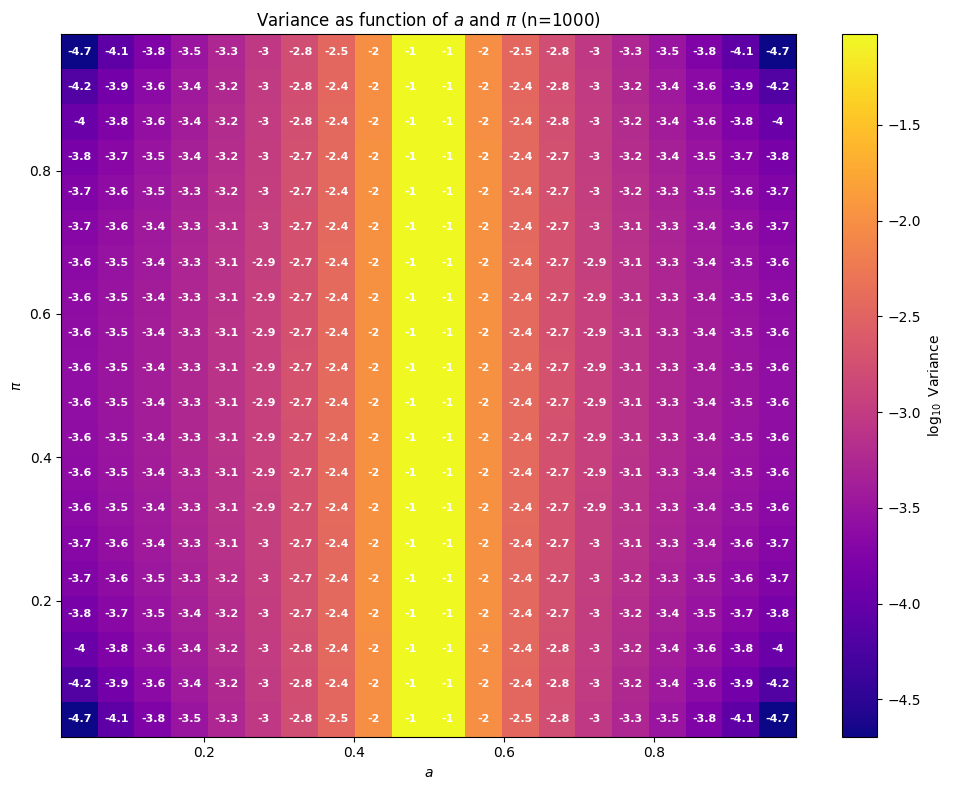
\includegraphics[width=\textwidth]{./heatmap.png}
    \caption{Variance of $\pi_{ML}$ as function of $a$ and $\pi$ for different values of $n$. Here, the values are log-scaled for better display. Note that we restrict $a\in [0.01, 0.99]$ and $\pi\in [0.01, 0.99]$ for the plot. Hence, very low values are expected whenever $a$ or $\pi$ exceeds these bounds.}
    \label{fig:variance_heatmap}
\end{figure}



\subsection{(g)}
\textit{Give an expression for the bias of this naive estimator. Is it asymptotically unbiased?}

We aim to recover the value of $\pi$ from direct questioning. 
However, persons belonging to the sensitive group will lie with probability $\ell$, whereas persons belonging to the non-sensitive group will answer truthfully and therefore lie with probability $0$.

Naivily, we could estimate the value of $\pi$ as the fraction of persons answering yes to the question:
\begin{equation*}
    \pi_\text{naive} = \frac{\sum_{i=1}^{n} X_i}{n}\;.
\end{equation*}

We can model the whether a person belongs to the sensitive group as a hidden variable $S_i \in \{0, 1\}$ with $S_i = 1$ describing that the person belongs to the sensitive group, and $S_i = 0$ describes that a person belongs to the non-sensitive group.

Naturally, we have that 
\begin{align*}
    P(S_i = 1) &= \pi \\
    P(S_i = 0) &= 1 - \pi
\end{align*}
which is distributed according to a Bernoulli distribution with parameter $p=\pi$.

We can now express the probability of a person answering yes or no to the question by marginalizing over the hidden variable $S_i$:
\begin{align*}
    P(X_i = 1) &= P(X_i = 1, S_i = 1) + P(X_i = 1, S_i = 0) \\
    &= \pi \cdot (1-\ell) + 0 \\
    P(X_i = 0) &= P(X_i = 0, S_i = 1) + P(X_i = 0, S_i = 0) \\
    &= \pi \cdot \ell + (1-\pi)\;.
\end{align*}

We verify that the probabilities are correct by adding both $P(X_i = 1)$ and $P(X_i = 0)$ and getting $1$:
\begin{align*}
    P(X_i = 1) + P(X_i = 0) &= \pi \cdot (1-\ell) + \pi \cdot \ell + (1-\pi) \\
    &= \pi (1-\ell + \ell) + 1- \pi \\
    &= \pi (1) + 1- \pi \\
    &= 1\;.
\end{align*}

We now compute the expeced value of the naive estimator of $\pi$ to check whether the estimator is unbiased.
We have
\begin{align*}
    \mathbb{E}[\pi_\text{naive}] &= \mathbb{E}\left[ \frac{\sum_{i=1}^{n} X_i}{n} \right] \\
    &= \frac{1}{n} \cdot \sum_{i=1}^{n} \mathbb{E}[X_i] \\
    &= \frac{1}{n} \cdot \sum_{i=1}^{n} \left( P(X_i = 1) \cdot 1 + P(X_i = 0) \cdot 0 \right) \\
    &= \frac{1}{n} \cdot \sum_{i=1}^{n} \left( P(X_i = 1) \right) \\
    &= \frac{1}{n} \cdot \sum_{i=1}^{n} \left( \pi \cdot (1-\ell) \right) \\
    &= \frac{1}{n} \cdot n \left( \pi \cdot (1-\ell) \right) \\
    &= \pi \cdot (1-\ell)\;. \stepandtag \label{eq:naive_expected_value}
\end{align*}

We can now use the expected value of $\pi_{\text{naive}}$ to compute the bias of the estimator:
\begin{align*}
    \text{Bias}(\pi_{\text{naive}}, \pi) &= {\left[ \mathbb{E}[\pi_{\text{naive}}] - \pi \right]}^2 \\
    &= {\left[ \pi \cdot (1-\ell) - \pi \right]}^2 \\
    &= {\left[ \pi - \pi \ell - \pi \right]}^2 \\
    &= {\left[ - \pi \ell \right]}^2 \\
    &= \pi^2 \ell^2\;. \stepandtag \label{eq:bias_naive}
\end{align*}

Therefore, only whenever $\ell = 0$, i.e., no one lies, is the naive estimator of $\pi$ is unbiased.
Otherwise, the estimator is biased towards and goes towards zero bias whenever either $\ell$ or $\pi$ goes to zero.


\subsection{(h)}
\textit{Derive expressions for the mean squared error (MSE) of the randomized response estimator and the naive estimator. Analyse the expressions to draw conclusions about when, depending on the relevant parameters $(\pi, a, \ell, n)$, one estimator should be favored over the other.}

We aim to compute the mean squared error of our two estimators of $\pi$.

% \begin{align*}
%     \text{MSE}(\pi_{\text{naive}}) &= \mathbb{E}\left[ {\left( \pi_{\text{naive}} - \pi \right)}^2 \right] \\
%     &= \mathbb{E} \left[ \pi_{\text{naive}}^2 + \pi^2 - 2\pi_{\text{naive}} \pi \right] \\
%     &= \mathbb{E} \left[ \pi_{\text{naive}}^2  \right] + \mathbb{E} \left[ \pi^2  \right] - \mathbb{E} \left[ 2\pi_{\text{naive}} \pi  \right] \\
%     &= \mathbb{E}\left[ {\left( \frac{\sum_{i=1}^{n} X_i}{n} \right)}^2 \right] + \pi^2 - 2 \pi \mathbb{E}\left[ \pi_{\text{naive}} \right] \\
%     &\overset{(\ref{eq:naive_expected_value})}{=} \mathbb{E}\left[ {\left( \frac{\sum_{i=1}^{n} X_i}{n} \right)}^2 \right] + \pi^2 - 2 \pi \left( \pi \cdot (1-\ell) \right) \\
%     &= \mathbb{E}\left[ {\left( \frac{\sum_{i=1}^{n} X_i}{n} \right)}^2 \right] + \pi^2 - 2 \pi^2 (1-\ell) \\
%     &= \mathbb{E}\left[ X_i \right]^2 + \pi^2 - 2 \pi^2 (1-\ell) \stepandtag \label{eq:mse_iid_assumption} \\
% \end{align*}
We use the Bias Variance decomposition to decompose the MSE into the bias and variance terms.\!\footnote{See \url{https://en.wikipedia.org/wiki/Mean_squared_error\#Proof_of_variance_and_bias_relationship}.}
Therefore, we simplify the MSE into 
\begin{align*}
    \text{MSE}(\hat{\pi}, \pi) &= \mathbb{E}\left[ {\left( \hat{\pi} - \mathbb{E}[\hat{\pi}] \right)}^2 \right] + {\left[ \mathbb{E}[\hat{\pi}] - \pi \right]}^2 \\
    &= \mathbb{V}\left[ \hat{\pi} \right] + {\left[ \mathbb{E}[\hat{\pi}] - \pi \right]}^2 \\
    &= \mathbb{V}\left[ \hat{\pi} \right] + \text{Bias}(\hat{\pi}, \pi) \\
\end{align*}
Therefore, we have
% \begin{align*}
%     \text{MSE}(\pi_{\text{naive}}, \pi) &= \mathbb{E}\left[ {\left( \mathbb{E}[\pi_{\text{naive}}] - \pi \right)}^2 \right] + {\left[ \mathbb{E}[\pi_{\text{naive}}] - \pi \right]}^2 \\
%     &= \mathbb{E}\left[ \mathbb{E}{[\pi_{\text{naive}}]}^2 + \pi^2 - 2\pi\mathbb{E}[\pi_{\text{naive}}]  \right] + {\left[ \mathbb{E}[\pi_{\text{naive}}] - \pi \right]}^2 \\
%     &= \mathbb{E}{[\pi_{\text{naive}}]}^2 + \mathbb{E}\left[ \pi^2  \right] - \mathbb{E}\left[ 2\pi\mathbb{E}[\pi_{\text{naive}}]  \right] + {\left[ \mathbb{E}[\pi_{\text{naive}}] - \pi \right]}^2 \\
%     &= \mathbb{E}{[\pi_{\text{naive}}]}^2 + \mathbb{E}\left[ \pi^2  \right] - 2\pi \mathbb{E}[\pi_{\text{naive}}] + {\left[ \mathbb{E}[\pi_{\text{naive}}] - \pi \right]}^2 \\
%     &\overset{(\ref{eq:naive_expected_value})}{=} {\left( \pi \cdot (1-\ell) \right)}^2 + \pi^2 - 2\pi \left( \pi \cdot (1-\ell) \right) + {\left[ \left( \pi \cdot (1-\ell) \right) - \pi \right]}^2 \\
%     &={\left( \pi \cdot (1-\ell) \right)}^2  + \pi^2 - 2\pi^2 \cdot (1-\ell) + {\left( \pi \cdot (1-\ell) \right)}^2 + \pi^2 - 2\pi\left( \pi \cdot (1-\ell) \right) \\
%     &= {\left( \pi \cdot (1-\ell) \right)}^2  + \pi^2 - 2\pi^2 \cdot (1-\ell) + {\left( \pi \cdot (1-\ell) \right)}^2 + \pi^2 - 2\pi^2 \cdot (1-\ell) \\
%     &= 2\pi^2 - 4\pi^2 \cdot (1-\ell) + 2{\left( \pi \cdot (1-\ell) \right)}^2  \\
%     &= 2\pi^2 - 4\pi^2 \cdot (1-\ell) + 2\pi^2 \cdot {(1-\ell)}^2  \\
%     &= 2\pi^2 \left( {(1-\ell)}^2 - 2(1-\ell) + 1 \right)  \\
%     &= 2\pi^2 \left( 1^2 + \ell^2 - 2\ell - 2 + 2\ell + 1 \right)  \\
%     &= 2\pi^2 \ell^2 
% \end{align*}
% Let us first compute $\mathbb{E}[\pi_\text{naive}^2]$ and ${\mathbb{E}[\pi_\text{naive}]}^2$.
% \begin{align*}
%     \mathbb{E}[\pi_\text{naive}^2] &= \mathbb{E} \left[ {\left( \frac{\sum_{i=1}^{n} X_i}{n} \right)}^2 \right] \\
%     &= \mathbb{E} \left[ {\left( \frac{\sum_{i=1}^{n} X_i}{n} \right)}^2 \right] \\
%     &= \mathbb{E} \left[ {\left( \frac{1}{n} \cdot \sum_{i=1}^{n} X_i \right)}^2 \right] \\
%     &= \mathbb{E} \left[ \frac{1}{n^2} {\left( \sum_{i=1}^{n} X_i \right)}^2 \right] \\
%     &= \frac{1}{n^2} \mathbb{E} \left[ {\left( \sum_{i=1}^{n} X_i \right)}^2 \right] \\
%     &= \frac{1}{n^2} \mathbb{E} \left[ n \cdot \mathbb{E}[X_i \cdot X_i] + (n^2 - n) \cdot \mathbb{E}[X_i \cdot X_j] \right] \\
%     &= \frac{1}{n^2} \mathbb{E} \left[ n \cdot \mathbb{E}[X_i^2] + (n^2 - n) \cdot \left( \mathbb{E}[X_i] + \mathbb{E}[X_j] \right) \right] \\
%     &= \frac{1}{n^2} \mathbb{E} \left[ n \cdot \mathbb{E}[X_i^2] + (n^2 - n) \cdot {\mathbb{E}[X_i]}^2 \right] \\
%     &= \frac{1}{n} \mathbb{E}[X_i^2] + \frac{n^2 - n}{n^2} \cdot {\mathbb{E}[X_i]}^2  \\
%     &= \frac{1}{n} \mathbb{E}[X_i^2] + \left( 1 - \frac{1}{n} \right) \cdot {\mathbb{E}[X_i]}^2  \\
%     &= \frac{1}{n} \mathbb{E}[X_i^2] + \left( \frac{n-1}{n} \right) \cdot {\mathbb{E}[X_i]}^2 \\
%     &= \frac{1}{n} \left[ P(X_i = 1) \cdot 1^2 + P(X_i = 0) \cdot 0^2 \right] + \left( \frac{n-1}{n}\right) \cdot {\left( P(X_i = 1) \cdot 1 + P(X_i = 0) \cdot 0 \right)}^2 \\
%     &= \frac{1}{n} \left[ P(X_i = 1)\right] + \left( \frac{n-1}{n} \right) \cdot {\left( P(X_i = 1) \right)}^2 \\
%     &= \frac{1}{n} \left[ \pi \cdot (1- \ell)\right] + \left( \frac{n-1}{n} \right) \cdot {\left( \pi \cdot (1- \ell) \right)}^2 \\
%     &= \frac{\pi \cdot (1- \ell)}{n} + \left( \frac{n-1}{n} \right) \cdot  \pi^2 \cdot {(1- \ell)}^2 
%     % &= \frac{1}{n} \left( \pi \cdot (1- \ell) + \left( n-1 \right) \cdot  \pi^2 \cdot {(1- \ell)}^2 \right) 
%     \stepandtag \label{eq:expectation_naive_x_i_square_outside} 
% \end{align*}

\begin{align*}
    \mathbb{V}[\pi_{\text{naive}}] &= \mathbb{V}\left[ \frac{\sum_{i=1}^{n} X_i}{n} \right] \\
    &= \frac{1}{n^2} \sum_{i=1}^{n} \mathbb{V}[X_i] \\
    &= \frac{1}{n^2} \sum_{i=1}^{n} \mathbb{E}[X_i^2] - {\mathbb{E}[X_i]}^2 \\
    &= \frac{1}{n^2} \sum_{i=1}^{n} \left[ P(X_i = 1) \right] - {\left( P(X_i = 1) \right)}^2 \\
    &= \frac{1}{n^2} \sum_{i=1}^{n} (\pi \cdot (1-\ell)) - {(\pi \cdot (1-\ell))}^2 \\
    &= \frac{n}{n^2} \left( (\pi \cdot (1-\ell)) - {(\pi \cdot (1-\ell))}^2 \right) \\
    &= \frac{\pi \cdot (1-\ell) - \pi^2 \cdot {(1-\ell)}^2}{n} \stepandtag \label{eq:variance_naive_x_i}
    % &= \frac{1}{n} \left( \pi \cdot (1-\ell) - \pi^2- \pi^2 \ell^2 \right) \\
\end{align*}

\begin{align*}
    \text{MSE}(\pi_{\text{naive}}, \pi) &= \mathbb{V}[\pi_{\text{naive}}] + \text{Bias}(\hat{\pi}, \pi) \\
    &\overset{(\ref{eq:variance_naive_x_i})}{=} \frac{\pi \cdot (1-\ell) - \pi^2 \cdot {(1-\ell)}^2}{n} + \text{Bias}(\hat{\pi}, \pi) \\
    &\overset{(\ref{eq:bias_naive})}{=} \frac{\pi \cdot (1-\ell) - \pi^2 \cdot {(1-\ell)}^2}{n} + \pi^2 \ell^2
    \;.
    % &= \frac{\pi \cdot (1-\ell) - \pi^2 \cdot {(1-\ell)}^2}{n} + {\mathbb{E}[\pi_{\text{naive}}]}^2 + \pi^2 - 2\pi \mathbb{E}\left[ \pi_{\text{naive}} \right] \\
    % &= \frac{\pi \cdot (1-\ell) - \pi^2 \cdot {(1-\ell)}^2}{n} + {\left( \pi \cdot (1-\ell) \right)}^2 + \pi^2 - 2\pi \pi \cdot (1-\ell) \\
    % &= \frac{\pi \cdot (1-\ell) - \pi^2 \cdot {(1-\ell)}^2}{n} + \pi^2 \cdot {(1-\ell)}^2 + \pi^2 - 2\pi^2 \cdot (1-\ell) \\
\end{align*}

Because the $\piml$ is an unbiased estimator of $\pi$, we have that $\text{Bias}(\piml, \pi) = 0$.
Therefore, we have
\begin{align*}
    \text{MSE}(\pi_{\text{ML}}, \pi) &= \mathbb{V}[\pi_{\text{ML}}] + \text{Bias}(\pi_{\text{ML}}, \pi) \\
    &= \mathbb{V}[\pi_{\text{ML}}] \\
    &\overset{(\ref{eq:variance_pi_ml})}{=} \frac{\pi - \pi^2}{n} + \frac{a - a^2}{{(2a-1)}^2 \cdot n}\;.
    % &\overset{(\ref{eq:variance_pi_ml})}{=} \frac{\pi - \pi^2}{n} + \frac{a - a^2}{(2^2a^2 +1^2 - 2a) \cdot n} \\
    % &\overset{(\ref{eq:variance_pi_ml})}{=} \frac{\pi - \pi^2}{n} - \frac{a - a^2}{2(a - \frac{1}{2} - 2a^2) \cdot n} \\
\end{align*}

First, we observe that whenever no-one lies ($\ell = 0$), the left side of the MSE of $\pi_{\text{naive}}$ is equal to the left side of the MSE of $\piml$. However, as the right side of the MSE of $\pi_{\text{naive}}$ is multiplied with $\ell^2$, the MSE is zero for $\ell = 0$, whereas the MSE of $\piml$ is non-zero, given $a\notin \{0, 1\}$. If $a\in \{0, 1\}$, then both estimators are equal w.r.t. the MSE.


% We now solve for both MSE expressions to be equal.
% \begin{align*}
%     \text{MSE}(\pi_{\text{naive}}, \pi) &= \text{MSE}(\pi_{\text{ML}}, \pi) \\
%     \frac{\pi \cdot (1-\ell) - \pi^2 \cdot {(1-\ell)}^2}{n} + \pi^2 \ell^2 & = \frac{\pi - \pi^2}{n} + \frac{a - a^2}{{(2a-1)}^2 \cdot n} &&\mid \cdot\  n \\
%     \pi \cdot (1-\ell) - \pi^2 \cdot {(1-\ell)}^2 + n \cdot \pi^2 \ell^2 & = \pi - \pi^2 + \frac{a - a^2}{{(2a-1)}^2} &&\mid \div \ \pi \\
%     (1-\ell) - \pi \cdot {(1-\ell)}^2 + n \cdot \pi \ell^2 & = 1 - \pi + \frac{a - a^2}{{(2a-1)}^2 \cdot \pi}  \stepandtag \label{eq:mse_equal} \;.
% \end{align*}

% First, we observe that Equation~\ref{eq:mse_equal} for the MSE of $\pi_{\text{naive}}$ increases w.r.t. $n$ whenever $\ell > 0$ and $\pi > 0$, whereas the MSE of $\piml$ does not depend on $n$.
% Therefore, this shows that with increasing sample size, the MSE of $\piml$ decreases faster than the MSE for $\pi_{\text{naive}}$. Therefore, for large sample size, $\piml$ should be preferred over $\pi_{\text{naive}}$.

Due to the complex expressions, finding the cut-off points for when both MSE expressions are equal --- and therefore finding whenever one estimator is better than the other analytically --- is very complicated.
While we have explained the trivial edge cases, whenever we have $a \notin \{0, 1\} \land \pi \notin \{0, 1\}$, we have no easy way to determine when which estimator is better than the other. To overcome this issue, we have computed the expected MSE for both estimators for a range of values for $a, \pi, \ell$, and $n$ and show the results in Figure~\ref{fig:mse_naive_better}. 
Figure~\ref{fig:mse_naive_better} clearly shows the complex, non-linear relationship between both MSE expression. 

First, it is clear that no single best estimator exists for all parameters. 
The shape of the region where $\pi_{naive}$ has a lower MSE than $\piml$ is quite clear:
whenever $\ell = 0$, the naive estimator is better than the ML estimator. Furthermore, whenever $\pi = 0$, the naive estimator is also better. Both cases make sense, as whenever no one lies, the naive estimator is the better estimator of the two.


\begin{figure}[htbp]
    \centering
    % 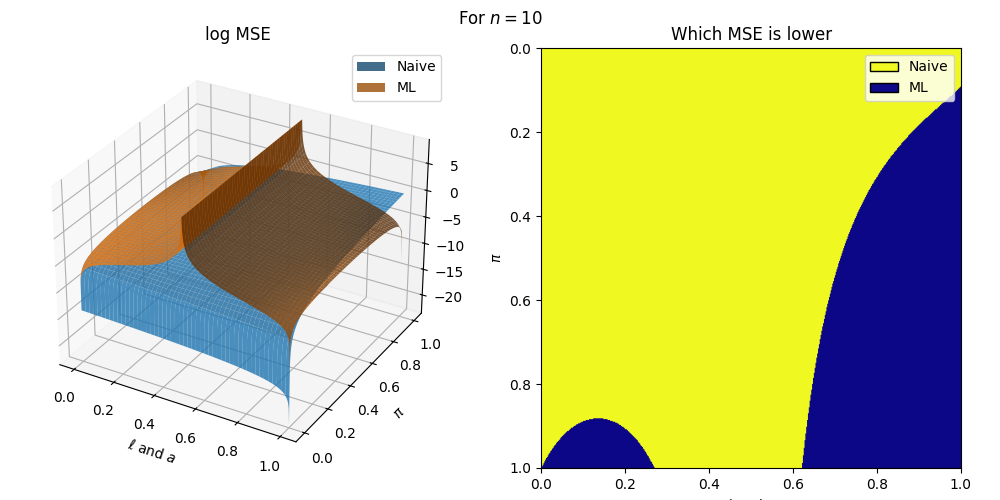
\includegraphics[width=0.7\textwidth]{MSE_naive_vs_ml_10.png}
    % 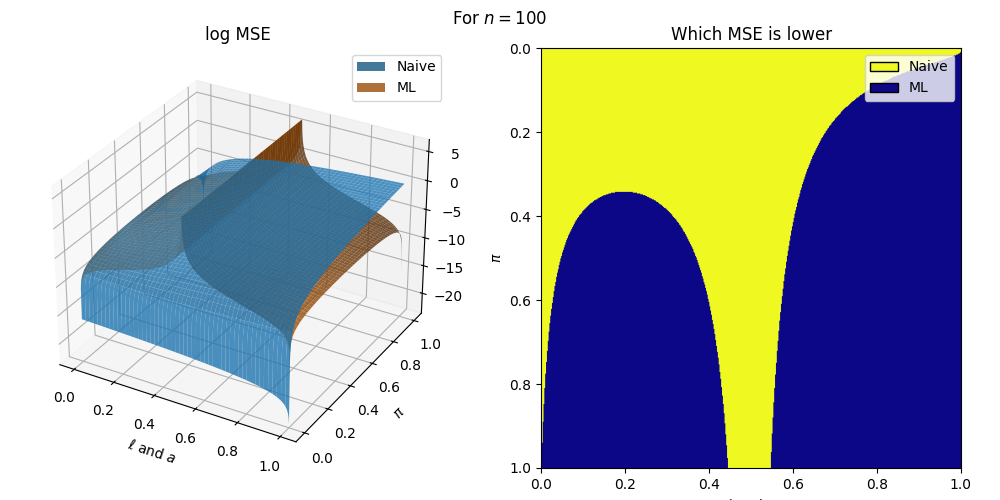
\includegraphics[width=0.7\textwidth]{MSE_naive_vs_ml_100.png}
    \subfloat[For $n = 10$]{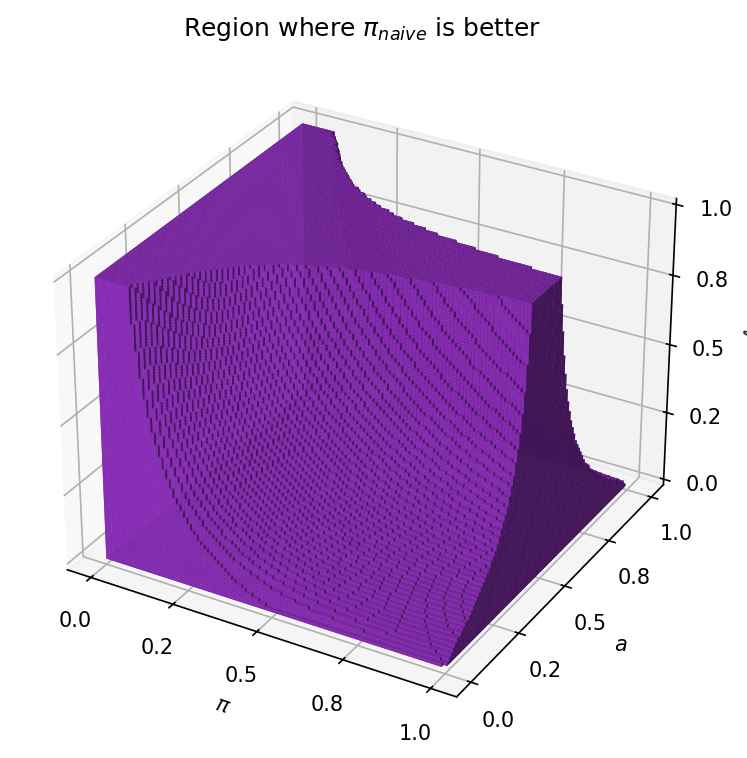
\includegraphics[width = 2.5in]{rregion_10.png}}
    % \subcaption{Meow}
    \subfloat[For $n = 100$]{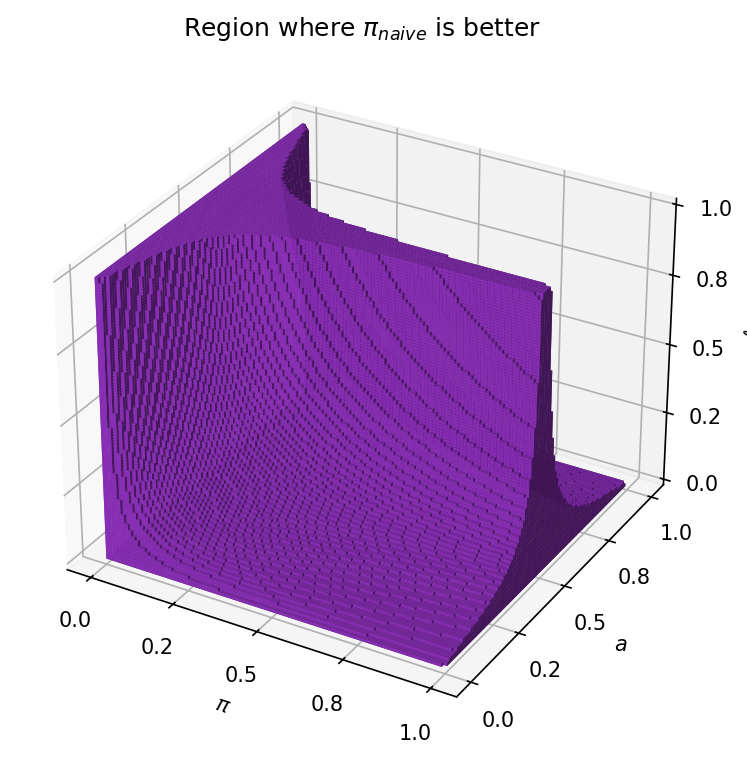
\includegraphics[width = 2.5in]{rregion_100.png}}\\
    \subfloat[For $n = 1\ 000$]{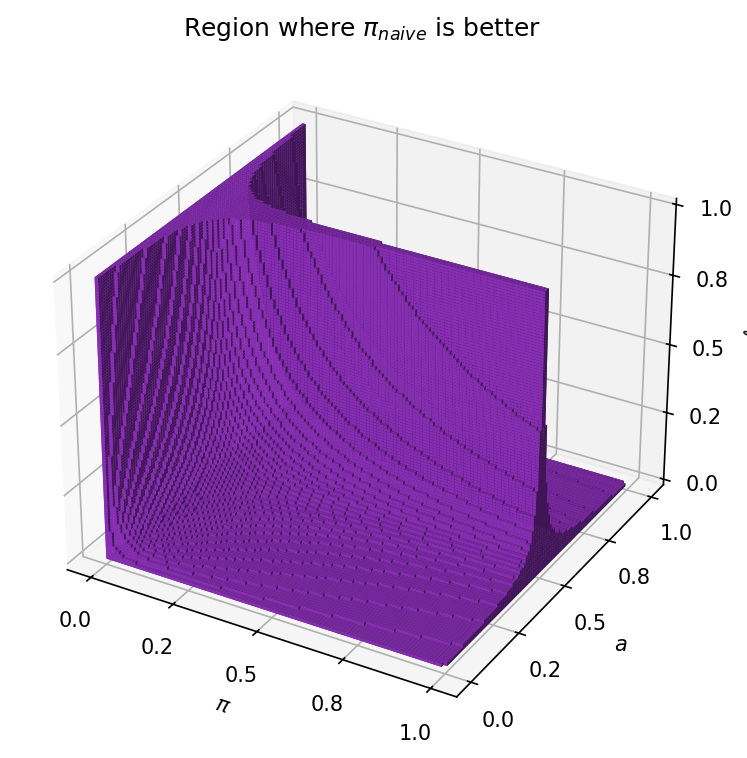
\includegraphics[width = 2.5in]{rregion_1000.png}}
    \subfloat[For $n = 10\ 000$]{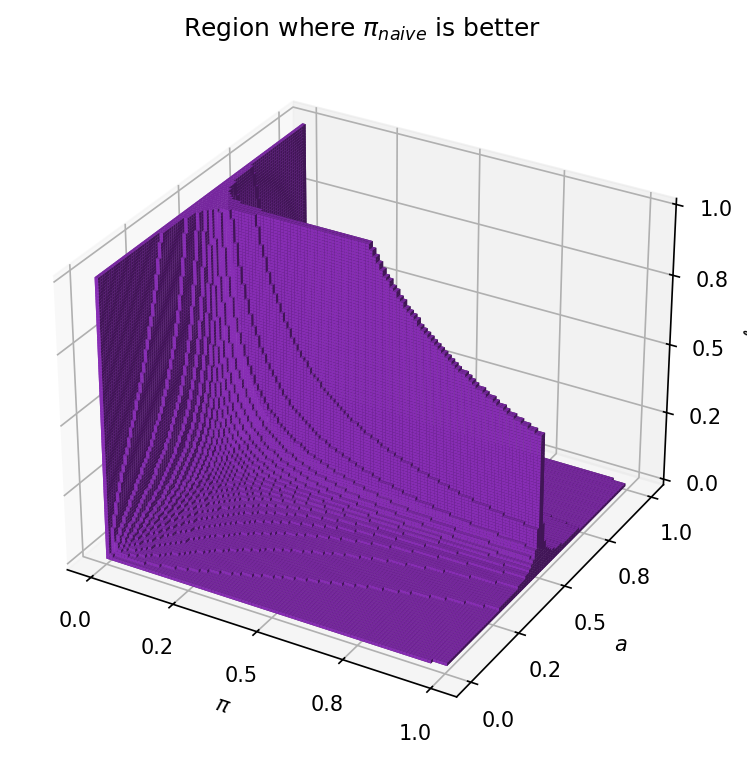
\includegraphics[width = 2.5in]{rregion_10000.png}} 
    \caption{Plots of the parameter space of $(\pi, a, \ell)$ for various sample sizes $n$. The purple voxels indicate for which parameters the MSE of $\pi_{naive}$ is lower than the MSE of $\piml$. Note that plot is mirrored around the $\ell$-axis at $a = 0.5$.}
    % \caption{In each subfigure, we plot the MSE of $\piml$ and $\pi_{\text{naive}}$ in 3D (left) and indicate with what parameters the MSE of $$}
    \label{fig:mse_naive_better}
\end{figure}

Figure~\ref{fig:mse_naive_better} also shows that whenever $a$ is close or equal to $0.5$, the naive estimator is the better solution. Note that while our plot shows that in the subplot (d), for some parameters which include $a=0.5$, the ML estimator is to be favored. This is not true, as it is simply an artefact of the plotting; We use only 100 points for each axis, and therefore the voxels are quite large. With increased resolution, the same plot would show that the naive estimator is the better solution for these parameters.

Lastly, for all other cases that we did not mention, the ML estimator is the better solution for large $n$. Refer to Figure~\ref{fig:mse_naive_better} for the exact shape. This is logical, as the MSE of the naive estimator has a part independent of $n$, whereas the MSE of the ML estimator is entirely divided by $n$. Thus, for large $n$, the ML estimator will go towards zero, whereas the naive estimator will remain constant.

% While Figure~\ref{} clearly shows the complex, non-linear relationship between both MSE expression, we vary the values of $a$ and $\ell$ together. This only shows a slice of the full parameter space. Therefore, we also plot the region where $\pi_{\text{naive}}$ has a lower MSE than $\piml$ in Figure~\ref{} when varying $\pi, a$, and $\ell$ independently.


% \begin{figure}[h]
%     \centering
%     % 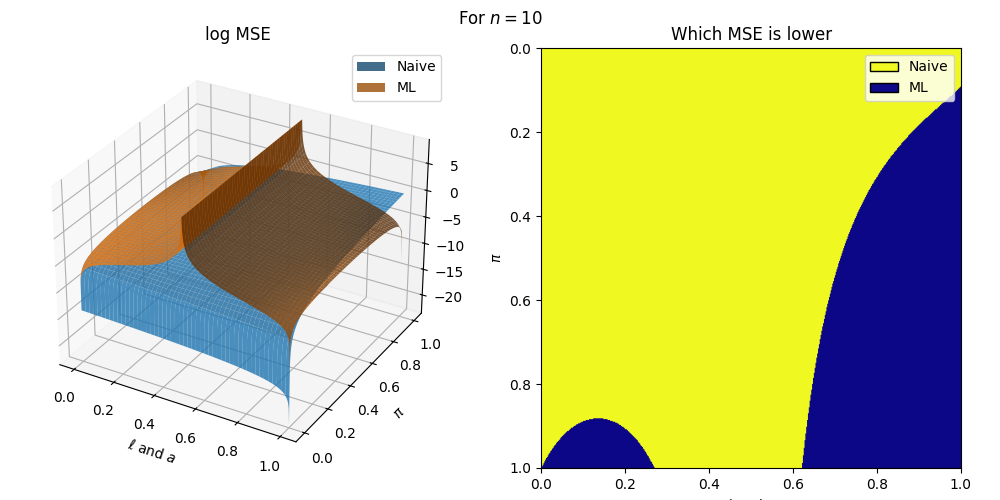
\includegraphics[width=0.7\textwidth]{MSE_naive_vs_ml_10.png}
%     % 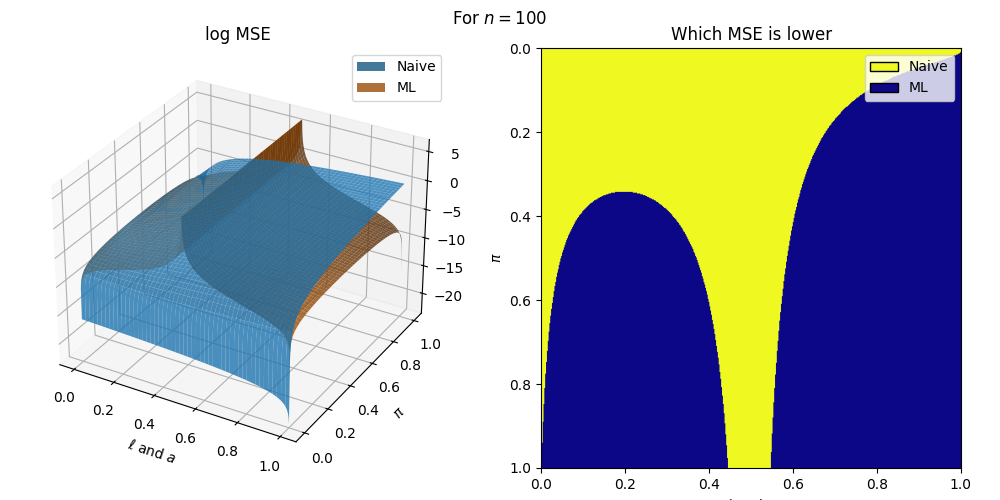
\includegraphics[width=0.7\textwidth]{MSE_naive_vs_ml_100.png}
%     \subfloat[For $n = 10$]{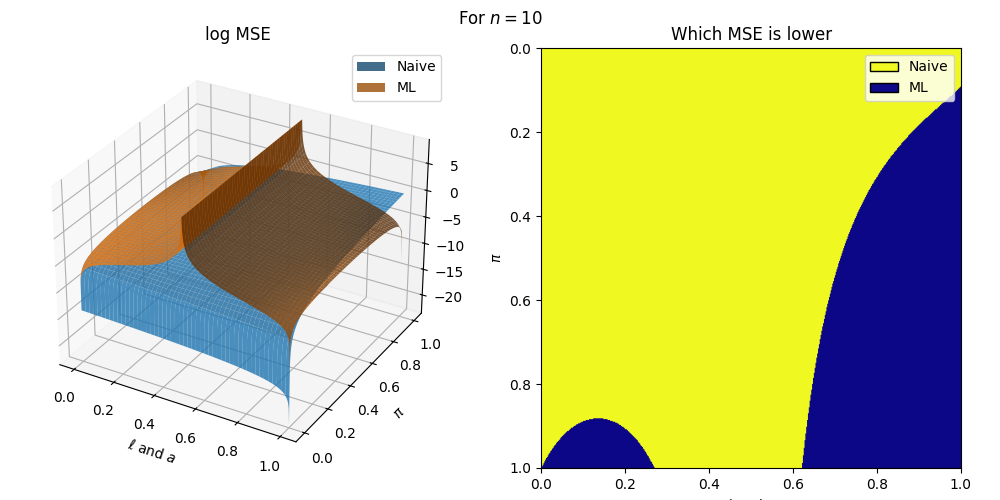
\includegraphics[width = 3in]{MSE_naive_vs_ml_10.png}}
%     % \subcaption{Meow}
%     \subfloat[For $n = 100$]{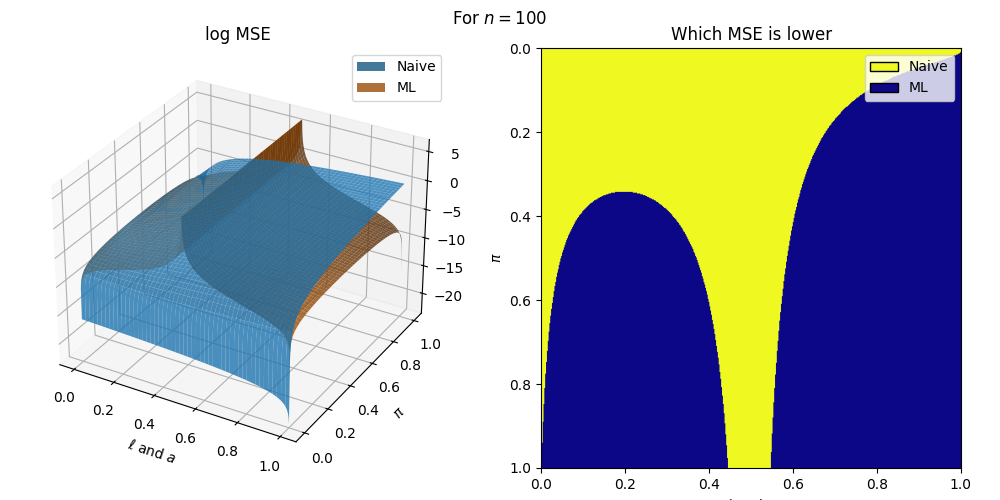
\includegraphics[width = 3in]{MSE_naive_vs_ml_100.png}}\\
%     \subfloat[For $n = 1\ 000$]{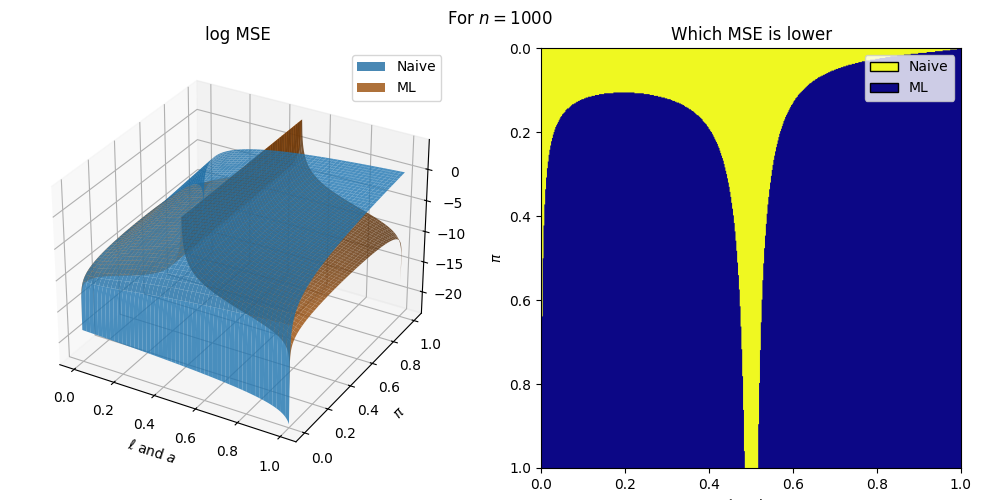
\includegraphics[width = 3in]{MSE_naive_vs_ml_1000.png}}
%     \subfloat[For $n = 10\ 000$]{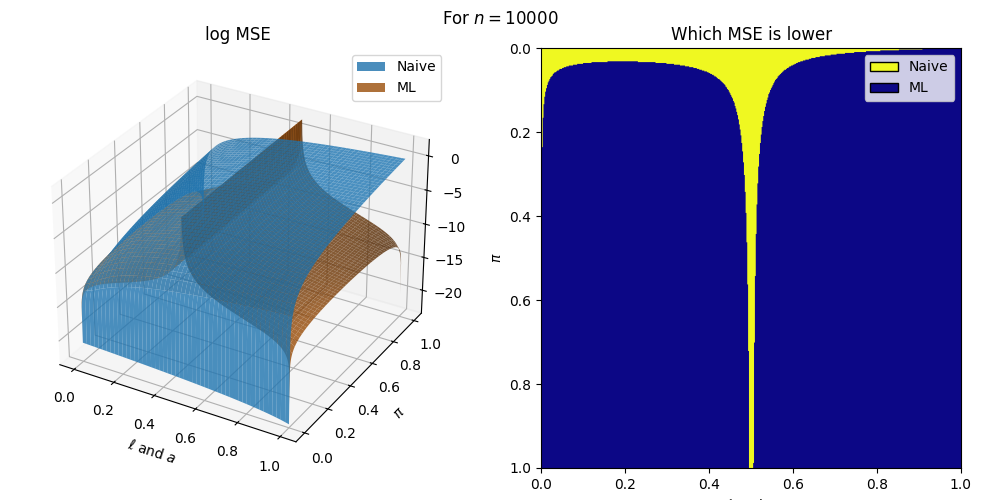
\includegraphics[width = 3in]{MSE_naive_vs_ml_10000.png}} 
%     \caption{\textbf{Left}: log MSE of $\piml$ and $\pi_{\text{naive}}$ in 3D. \textbf{Right}: The region indicating whenever an estimator has a lower MSE than the other. In this figure, we link $a$ and $\ell$ together (they are both on the same axis) as the MSE for both estimators depends on only one of them.}
%     % \caption{In each subfigure, we plot the MSE of $\piml$ and $\pi_{\text{naive}}$ in 3D (left) and indicate with what parameters the MSE of $$}
%     \label{fig:mse_naive_vs_ml}
% \end{figure}



% Let us now analyze the critical points of both MSE expressions, i.e., whenever they are both equal, to determine when one estimator has a lower MSE than the other.

% Let us first solve for $\ell$:
% \begin{align*}
%     \text{MSE}(\pi_{\text{naive}}, \pi) &= \text{MSE}(\pi_{\text{ML}}, \pi) \\
%     \frac{\pi \cdot (1-\ell) - \pi^2 \cdot {(1-\ell)}^2}{n} + \pi^2 \ell^2 &= \frac{\pi - \pi^2}{n} + \frac{a - a^2}{{(2a-1)}^2 \cdot n} \\
%     \frac{\pi \cdot (1-\ell) - \pi^2 \cdot {(1-\ell)}^2}{n} &= \frac{\pi - \pi^2}{n} + \frac{a - a^2}{{(2a-1)}^2 \cdot n} -  \pi^2 \ell^2 \\
%     \pi \cdot (1-\ell) - \pi^2 \cdot {(1-\ell)}^2 &= \pi - \pi^ 2+ \frac{a - a^2}{{(2a-1)}^2} -  n\cdot\pi^2 \ell^2 \\ 
%     \pi - \ell \pi - \pi^2 \cdot \left( 1 + \ell^2 - 2\ell \right) &= \pi - \pi^ 2+ \frac{a - a^2}{{(2a-1)}^2} -  n\cdot\pi^2 \ell^2 &&\mid \div\ \pi \\ 
%     1 - \ell - \pi \cdot \left( 1 + \ell^2 - 2\ell \right) &= 1 - \pi + \frac{a - a^2}{{(2a-1)}^2\cdot\pi} -  n\cdot\pi \ell^2 \\ 
%     \ell + \pi\ell^2 + 2\ell \pi + n\cdot\pi \ell^2  &= \frac{a - a^2}{{(2a-1)}^2\cdot\pi}  \\ 
%     \ell \left( 1 + 2 \pi \right) + \ell^2 \left( \pi + n \cdot \pi \right)  &= \frac{a - a^2}{{(2a-1)}^2\cdot\pi}  \\ 
%     \ell \frac{\left( 1 + 2 \pi \right)}{\left( \pi + n \cdot \pi \right)}  + \ell^2  &= \frac{a - a^2}{{(2a-1)}^2\cdot\pi \cdot \left( \pi + n \cdot \pi \right)}  \\ 
%     \ell^2 + \ell \frac{\left( 1 + 2 \pi \right)}{\left( \pi + n \cdot \pi \right)} - \frac{a - a^2}{{(2a-1)}^2\cdot\pi \cdot \left( \pi + n \cdot \pi \right)}  &= 0  \\ 
%     \ell^2 + \ell \frac{\left( 1 + 2 \pi \right)}{\pi\left( n+1 \right)} - \frac{a - a^2}{{(2a-1)}^2\cdot\pi^2 \cdot \left( n+1 \right)}  &= 0  \\ 
% \end{align*}
% where the equation trivialy holds for the following points:
% \begin{itemize}
%     \item $\ell = 0, a = 1, \pi\neq 0$
%     \item $\ell = 0, a = 0, \pi \neq 0$
%     \item $\ell = 0, n=\infty, a\neq 0.5, \pi \neq 0$
% \end{itemize}
% however, for points, we need to solve the quadratic equation. To this end, we use the quadratic formula.
% We set 
% \begin{equation*}
%     p = \frac{\left( 1 + 2 \pi \right)}{\left( \pi + n \cdot \pi \right)} \\
% \end{equation*}
% and 
% \begin{equation*}
%     q = - \frac{a - a^2}{{(2a-1)}^2\cdot\pi^2 \cdot \left( n+1 \right)}\;.
% \end{equation*}
% We therefore have
% \begin{align*}
%     \ell_1, \ell_2 &= - \frac{p}{2} \pm \sqrt{{\left( \frac{p}{2} \right)}^2 - q} \\
%     &= -\frac{ 1 + 2 \pi }{2 \left( \pi + n \cdot \pi \right)} \pm \sqrt{\frac{{\left( 1 + 2 \pi \right)}^2}{{2\left( \pi + n \cdot \pi \right)}^2} + \frac{a - a^2}{{(2a-1)}^2\cdot\pi^2 \cdot \left( n+1 \right)}} \\
%     % &= -\frac{ 1 + 2 \pi }{2 \left( \pi + n \cdot \pi \right)} \pm \sqrt{\frac{{\left( 1 + 2 \pi \right)}^2}{{2\left( \pi + n \cdot \pi \right)}^2} + \frac{a - a^2}{\left( 2^2a^2+1 - 2a \right)\cdot\pi^2 \cdot \left( n+1 \right)}} \\
% \end{align*}

% \begin{align*}
%     \text{MSE}(\pi_{\text{naive}}, \pi) &= \mathbb{E}\left[ {\left( \pi_{\text{naive}} - \mathbb{E}[\pi_{\text{naive}}] \right)}^2 \right] + {\left[ \mathbb{E}[\pi_{\text{naive}}] - \pi_{\text{naive}} \right]}^2 \\
%     &= \mathbb{E}\left[ \mathbb{E}{[\pi_{\text{naive}}]}^2 + \pi_{\text{naive}}^2 - 2\pi_{\text{naive}}\mathbb{E}[\pi_{\text{naive}}]  \right] + {\left[ \mathbb{E}[\pi_{\text{naive}}] - \pi \right]}^2 \\
%     &= \mathbb{E}{[\pi_{\text{naive}}]}^2 + \mathbb{E}\left[ \pi_{\text{naive}}^2  \right] -   2\pi_{\text{naive}}\mathbb{E}[\pi_{\text{naive}}] + \mathbb{E}{[\pi_{\text{naive}}]}^2 + \pi^2 - 2\pi  \mathbb{E}[\pi_{\text{naive}}] \\
%     % &= 2\mathbb{E}{[\pi_{\text{naive}}]}^2 + \mathbb{E}\left[ \pi_{\text{naive}}^2  \right] + \pi^2 - 4\pi  \mathbb{E}[\pi_{\text{naive}}] \\
%     &= 2\mathbb{E}{[\pi_{\text{naive}}]}^2 + \mathbb{E}\left[ \pi_{\text{naive}}^2  \right] + \pi^2 + \mathbb{E}[\pi_{\text{naive}}]\cdot(2\pi - 2 \pi_{\text{naive}}) \\
%     % &=  2\mathbb{E}{[\pi_{\text{naive}}]}^2 + \mathbb{E}\left[ \pi_{\text{naive}}^2  \right] + \pi^2 + \mathbb{E}[\pi_{\text{naive}}]\cdot(2\pi - 2 \pi_{\text{naive}}) \\
%     &\overset{(\ref{eq:expectation_naive_x_i_square_outside})}{=}  2\mathbb{E}{[\pi_{\text{naive}}]}^2 + \frac{\pi \cdot (1- \ell)}{n} + \left( \frac{n-1}{n} \right) \cdot  \pi^2 \cdot {(1- \ell)}^2 + \pi^2 - \mathbb{E}[\pi_{\text{naive}}]\cdot(2\pi + 2 \pi_{\text{naive}}) \\
%     % &\overset{(\ref{eq:expectation_naive_x_i_square_outside})}{=} 2\mathbb{E}{[\pi_{\text{naive}}]}^2 + \frac{\pi \cdot (1- \ell)}{n} + \left( \frac{n-1}{n} \right) \cdot  \pi^2 \cdot {(1- \ell)}^2 + \\
%     &\overset{(\ref{eq:naive_expected_value})}{=} 2 {\left[ \pi \cdot (1-\ell) \right]}^2 + \frac{\pi \cdot (1- \ell)}{n} + \left( \frac{n-1}{n} \right) \cdot  \pi^2 \cdot {(1- \ell)}^2 + \pi^2 -\left( \pi \cdot (1-\ell) \right)\cdot(2\pi + 2 \pi_{\text{naive}}) \\
%     &\overset{(\ref{eq:naive_expected_value})}{=} 2 {\left[ \pi \cdot (1-\ell) \right]}^2 + \frac{\pi \cdot (1- \ell)}{n} + \left( \frac{n-1}{n} \right) \cdot  \pi^2 \cdot {(1- \ell)}^2 + \pi^2 - \left( \pi \cdot (1-\ell) \right)\cdot(2\pi + 2 \pi_{\text{naive}}) \\
%     &= 2 {\left[ \pi \cdot (1-\ell) \right]}^2 + \frac{\pi \cdot (1- \ell)}{n} + \left( \frac{n-1}{n} \right) \cdot  \pi^2 \cdot {(1- \ell)}^2 + \pi^2 - 2\pi \cdot (1-\ell) \cdot(\pi +  \pi_{\text{naive}}) \\
%     &= 2 \pi^2 \cdot {(1-\ell)}^2 + \frac{\pi \cdot (1- \ell)}{n} + \left( \frac{n-1}{n} \right) \cdot  \pi^2 \cdot {(1- \ell)}^2 + \pi^2 - 2\pi \cdot (1-\ell) \cdot(\pi +  \pi_{\text{naive}}) \\
%     &= \left( 1-\ell \right) \cdot \left( 2\pi^2 \cdot (1-\ell) + \frac{\pi}{n} + \left( \frac{n-1}{n} \right) \cdot  \pi^2 \cdot {(1- \ell)} - 2\pi (\pi +  \pi_{\text{naive}}) \right) \\
%     &= \left( 1-\ell \right) \cdot \left( 2\pi^2 \cdot (1-\ell) + \frac{\pi}{n} + \left( \frac{n-1}{n} \right) \cdot  \pi^2 \cdot {(1- \ell)} - 2\pi^2 -  2\pi\pi_{\text{naive}} \right) \\
%     &= \pi \cdot \left( 1-\ell \right) \cdot \left( 2\pi \cdot (1-\ell) + \frac{1}{n} + \left( \frac{n-1}{n} \right) \cdot  \pi \cdot {(1- \ell)} - 2\pi -  2\pi_{\text{naive}} \right) \\
%     &= \pi \cdot \left( 1-\ell \right) \cdot \left( 2\pi -2\pi \ell + \frac{1}{n} + \left( \frac{n-1}{n} \right) \cdot  \pi \cdot {(1- \ell)} - 2\pi -  2\pi_{\text{naive}} \right) \\
%     % &= 2 \pi^2 \cdot {(1-\ell)}^2 + \frac{\pi \cdot (1- \ell)}{n} + \left( \frac{n-1}{n} \right) \cdot  \pi^2 \cdot {(1- \ell)}^2 + \pi^2 + 2 \pi^2 \cdot (1-\ell) - 2 \pi_{\text{naive}} \pi \cdot (1-\ell) \\
%     % &= \pi^2 \left( 2 \cdot {(1-\ell)}^2 + \left( \frac{n-1}{n} \right)\cdot {(1-\ell)}^2 + 1 + 2 \cdot (1-\ell)  \right) + \frac{\pi \cdot (1- \ell)}{n} - 2 \pi_{\text{naive}} \pi \cdot (1-\ell) \\
%     % &= \pi^2 \left( 2- 2\ell^2 + \left( \frac{n-1}{n} \right) - \left( \frac{(n-1) \ell}{n} \right) + 1 + 2-2\ell  \right) + \frac{\pi \cdot (1- \ell)}{n} - 2 \pi_{\text{naive}} \pi \cdot (1-\ell) \\
%     % &= \pi^2 \left( 5- 2\ell^2 + \left( \frac{n-1}{n} \right) - \left( \frac{(n-1) \ell}{n} \right) -2\ell  \right) + \frac{\pi \cdot (1- \ell)}{n} - 2 \pi_{\text{naive}} \pi \cdot (1-\ell) \\
%     % % &= 2 \pi^2 \cdot {(1-\ell)}^2 + \frac{\pi \cdot (1- \ell)}{n} + \left( \frac{n-1}{n} \right) \cdot  \pi^2 \cdot {(1- \ell)}^2 + \pi^2 - 4\pi^2 \cdot (1-\ell) \\
% \end{align*}

% \pagebreak
% We have
% \todo[inline]{This is for the non-naive estimator.}
% \begin{align*}
%     \text{MSE}(\pi_\text{naive}) &= \mathbb{E}\left[ {(\pi_\text{naive} - \pi)}^2 \right] \\
%     &= \mathbb{E} \left[ {\left( \frac{\sum_{i=1}^{n} X_i}{n} - \pi \right)}^2 \right] \\
%     &= \mathbb{E} \left[ \frac{\sum_{i=1}^{n} X_i^2}{n^2} + \pi^2 - 2\pi\frac{\sum_{i=1}^{n} X_i}{n}  \right] \\
%     &= \mathbb{E} \left[ \frac{\sum_{i=1}^{n} X_i^2}{n^2} \right] + \mathbb{E} \left[ \pi^2 \right] - \mathbb{E} \left[ 2\pi\frac{\sum_{i=1}^{n} X_i}{n} \right] \\
%     &= \frac{1}{n^2} \sum_{i=1}^{n} \mathbb{E} \left[ X_i^2 \right] + \pi^2 - \frac{2 \pi}{n} \sum_{i=1}^{n} \mathbb{E}[X_i] \\
%     &\overset{(\ref{eq:expectation_naive_x_i_square_inside})}{=} \frac{1}{n^2} \sum_{i=1}^{n} \left[ (1-a) + (2a - 1) \cdot \pi \right] + \pi^2 - \frac{2 \pi}{n} \sum_{i=1}^{n} \mathbb{E}[X_i] \\
%     &= \frac{1}{n} \left[ (1-a) + (2a - 1) \cdot \pi \right] + \pi^2 - \frac{2 \pi}{n} \sum_{i=1}^{n} \mathbb{E}[X_i] \\
%     &\overset{(\ref{eq:expectation_naive_x_i_square_outside})}{=} \frac{1}{n} \left[ (1-a) + (2a - 1) \cdot \pi \right] + \pi^2 - \frac{2 \pi}{n} \sum_{i=1}^{n} \left[ 1 + \pi \left(6a - 4a^2 - 2 \right) + \pi^2 (4 a^2 - 4 a + 1) - 2a + a^2 \right] \\
%     &= \frac{1}{n} \left[ (1-a) + (2a - 1) \cdot \pi \right] + \pi^2 - 2 \pi \cdot \left[ 1 + \pi \left(6a - 4a^2 - 2 \right) + \pi^2 (4 a^2 - 4 a + 1) - 2a + a^2 \right] \\
%     &= \frac{(1-a)}{n} + \frac{(2a - 1) \cdot \pi }{n}
%      + \pi^2 - 2 \pi 
%     - 2 \pi^2 \left(6a - 4a^2 - 2 \right) - 2 \pi^3 (4 a^2 - 4 a + 1) + 4 \pi a - 2 \pi a^2  \\
%     &= \pi \left( \frac{2a -1}{n} - 2 + 4a - 2a^2 \right) + \pi^2 (1 - 12a + 4a^2 - 4) + \pi^3 ()
% \end{align*}


\pagebreak
\section{Problem 2}


We have implemented the given formulas for estimating the population size $\hat{N}$ and its variance $\hat{\sigma}_{\hat{N}}$ given some probability distributions from which we sample the probability of catching one animal. 
We have run the Monte-Carlo simulations for 1000 runs for each given probabiliy distribution and report on the computed values in Table~\ref{tab:problem_2_results_uniform_0_01} for $p_i \sim U(0, 0.01)$, Table~\ref{tab:problem_2_results_uniform_0_02} for $p_i \sim U(0, 0.02)$, Table~\ref{tab:problem_2_results_beta_1_3} for $p_i \sim 0.02 \cdot \mathrm{Beta}(1, 3)$, and Table~\ref{tab:problem_2_results_beta_2_2} for $p_i \sim 0.01 \cdot \mathrm{Beta}(2, 2)$.

Note that for the sake of ease of comparison, we report on $\hat{\sigma}_{\hat{N}} = \sqrt{\hat{\sigma}_{\hat{N}}^2}$ instead of the variance $\hat{\sigma}_{\hat{N}}^2$ as it allows us to directly compare it with the reported standard deviations of the other parameters.

% \todo[inline]{Compute expected value of catching one animal by 
% $\mathbb{E}[\Pr(X_i^t = 1)] = \int_0^1 Pr(p \leq q) dq\quad p \sim \Pr(\cdot) \Leftrightarrow \int_0^1 \int_0^q Pr(p' = p) dp' dq$ (something around double integral...)}

In this question, we are interested in the differences that arise from the different probability distributions, besides their performances. 
% Therefore, we will set out focus on their comparisons.

We first plot the probability distribution for the four probability distributions that we are investigating in Figure~\ref{fig:probability_density_functions}. From that figure, we hypothesize that the expected value of catching one animal is not the same for all four probability distributions. Therefore, let us first compute the expected value of catching one animal for each probability distribution. 

For the uniform distribution $U(0, a)$, with $a\in \mathbb{R}\setminus \{0\}$, we have:
\begin{align*}
    \mathbb{E}_{p \sim U(0, a)}[X_i^t] &= \mathbb{E}_{p \sim U(0, a), q\sim U(0, 1)}\left[ q \leq p \right] \\
    &= \mathbb{E}_{p \sim U(0, a)}\left[ \mathbb{E}_{q\sim U(0, 1)} \left[ q \leq p \right] \right] \\
    &= \int_0^a f_p(p) \cdot \mathbb{E}_{q\sim U(0, 1)} \left[ q \leq p \right] \  dp \\ 
    &= \int_0^a \frac{1}{a} \cdot \mathbb{E}_{q\sim U(0, 1)} \left[ q \leq p \right] \  dp \\ 
    &= \frac{1}{a} \int_0^a \mathbb{E}_{q\sim U(0, 1)} \left[ q \leq p \right] \  dp \\ 
    &= \frac{1}{a} \int_0^a \int_0^1 f_q(q) \cdot \mathbb{1}\{q \leq p\} \ dq \  dp \\
    &= \frac{1}{a} \int_0^a \int_0^1 1 \cdot \mathbb{1}\{q \leq p\} \ dq \  dp \\
    % &= \frac{1}{a} \int_0^a \int_0^1 \mathbb{1}\{q \leq p\} \ dq \  dp \\
    &= \frac{1}{a} \int_0^a \int_0^p 1 \ dq \  dp \\
    &= \frac{1}{a} \int_0^a {\left[ q \right]}_0^p \  dp \\
    &= \frac{1}{a} \int_0^a p \  dp \\
    &= \frac{1}{a} {\left[ \frac{p^2}{2} \right]}_0^a \\
    &= \frac{1}{a} \frac{a^2}{2} \\
    &= \frac{a}{2} \;.
\end{align*}

It naturally follows that 
\begin{equation}
    \mathbb{E}_{p \sim U(0, 0.01)}[X_i^t] = 0.005
    \label{eq:expectation_xi_u01}
\end{equation}
and
\begin{equation}
    \mathbb{E}_{p \sim U(0, 0.02)}[X_i^t] = 0.01\;.
    \label{eq:expectation_xi_u02}
\end{equation}

For $p\sim \mathrm{Beta}(\cdot)$, we have:
\begin{align*}
    \mathbb{E}_{p \sim \mathrm{Beta}(\alpha, \beta)}[X_i^t] &= \mathbb{E}_{p \sim \mathrm{Beta}(\alpha, \beta), q\sim U(0, 1)}\left[ q \leq p \right] \\
    &= \mathbb{E}_{p \sim \mathrm{Beta}(\alpha, \beta)}\left[ \mathbb{E}_{q\sim U(0, 1)} \left[ q \leq p \right] \right] \\
    &= \int_0^1 f_{\mathrm{Beta}(\alpha, \beta)}(p) \cdot \mathbb{E}_{q\sim U(0, 1)} \left[ q \leq p \right]\ dp\\
    &= \int_0^1 f_{\mathrm{Beta}(\alpha, \beta)}(p) \cdot \int_0^1 f_q(q) \cdot \mathbb{1}\{q \leq p\} \ dq \ dp\\
    &= \int_0^1 f_{\mathrm{Beta}(\alpha, \beta)}(p) \cdot p \  dp \\
    &= \mathbb{E}_{X\sim \mathrm{Beta}(\alpha, \beta)}\left[ X \right] \\
    &= \frac{\alpha}{\alpha + \beta}\;. 
    \stepandtag \label{eq:expectation_beta}
\end{align*}
Note that if $p\sim a \cdot \mathrm{Beta}(\cdot)$ with $a\in \mathbb{R} \setminus \{0\}$, we can just multiply Equation~\ref{eq:expectation_beta} with $a$ due to the properties of the expectation and the integrals. $a$ would be contained in the density function as a multiplicative factor, and thus, we can extract it.
Note that I got the expectation of the Beta distribution from wikipedia.\!\footnote{\url{https://en.wikipedia.org/wiki/Beta_distribution}}

Therefore, it follows that 
\begin{equation}
    \mathbb{E}_{p \sim 0.02 \cdot \mathrm{Beta}(1, 3)}[X_i^t] = 0.02 \cdot \frac{1}{4} = 0.005
    \label{eq:expectation_xi_beta13}
\end{equation}
and 
\begin{equation}
    \mathbb{E}_{p \sim 0.01 \cdot \mathrm{Beta}(2, 2)}[X_i^t] = 0.01 \cdot \frac{1}{2} = 0.005\;.
    \label{eq:expectation_xi_beta22}
\end{equation}

The usefulness of Equation~\ref{eq:expectation_xi_u01}--\ref{eq:expectation_xi_u02} and Equation~\ref{eq:expectation_xi_beta13}--{\ref{eq:expectation_xi_beta22}} expected values will become clear in the next section.

\vspace{1em}

\begin{figure}[t]
    \centering
    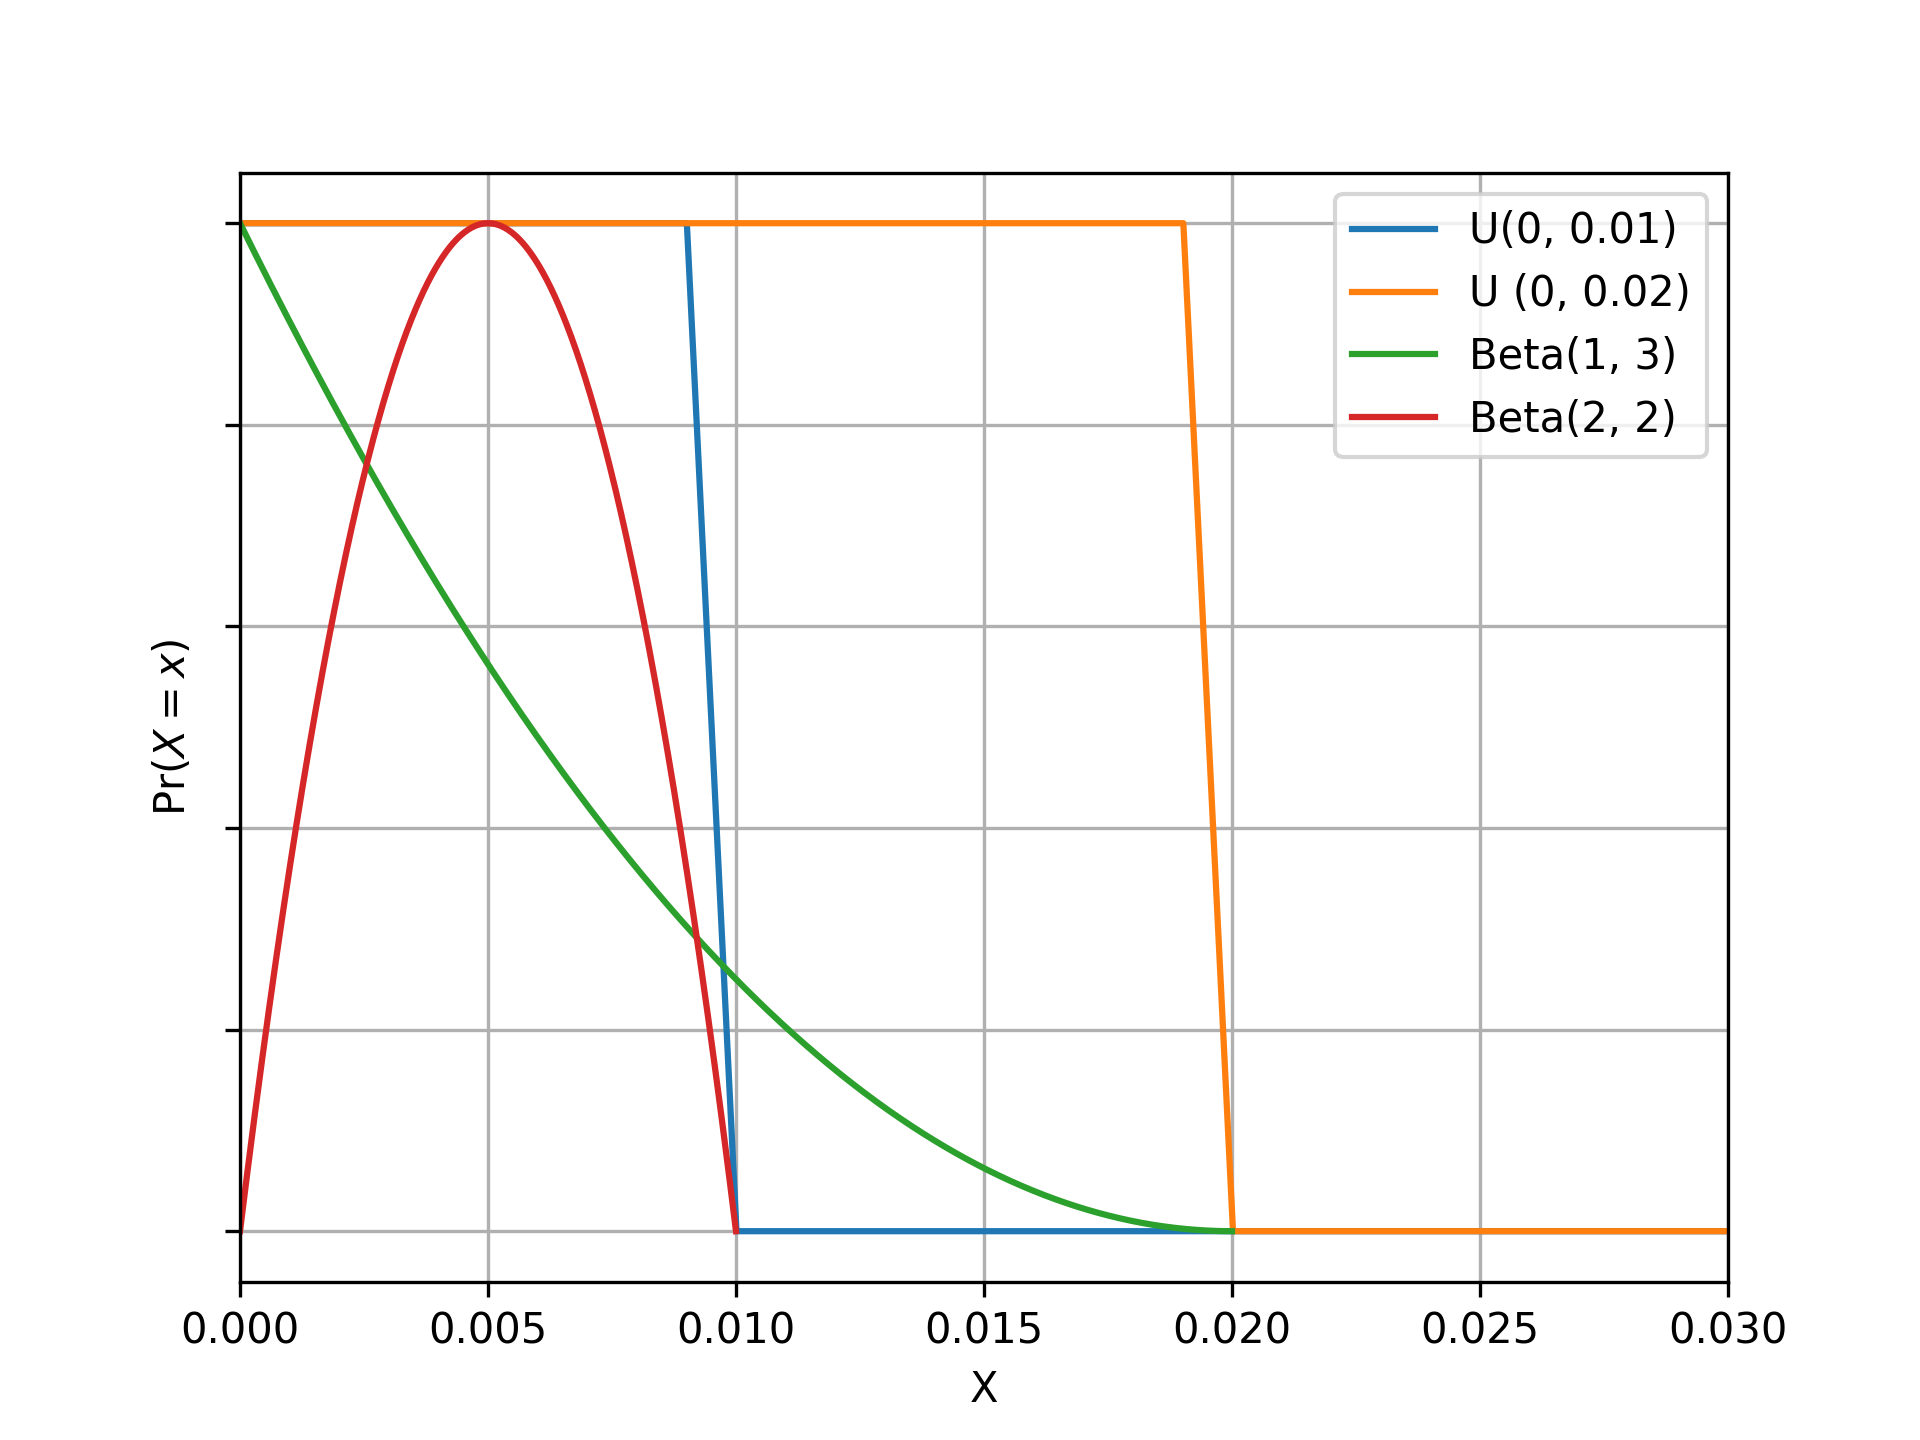
\includegraphics[width=0.5\textwidth]{probability_density_functions.png}
    \caption{Probability density functions for the four different probability distributions. We normalize the probability density functions to have a maximum value of 1 for each distribution as we are interested in the relative differences between the different distributions. While the height of the pdfs are not to scale, their shape are.}
    \label{fig:probability_density_functions}
\end{figure}


\textbf{Expected Behavior.}
Before discussing the results of the Monte-Carlo simulations in detail, let us first investigate the expected behavior of the simulations.

We have computed the expected number of times an animal is being catched at each time step. Recall that the expected values for $X_i^t$ is $0.005$ for all given distributions, except when $p\sim U(0, 0.01)$, as in that setting, the expected value rises to $0.01$.

Concretely, this means that when using $U(0, 0.01)$ as the probability to catch an animal, the number of times an animal is being catched is twice as high as when using the three other probability distribution.
Therefore, we expect the estimations of $\hat{N}$ and $\sigma_{\hat{N}}$ to be better when using $p\sim U(0, 0.01)$ as oposed to the other distributions.

Trivially, as the expected behavior of the three other distributions are identical, we expect the estimations of $\hat{N}$ and $\sigma_{\hat{N}}$ to be very identical up to the effect of the randomness introduced by the Monte-Carlo simulations.

\begin{table}[t]
    \centering 
    \caption*{$p_i \sim U(0, 0.01)$}
    \begin{tabular}{c c|c c c}
        \toprule
        & & \multicolumn{1}{|c|}{${N}=500$} & \multicolumn{1}{c|}{${N}=1000$} & \multicolumn{1}{c}{${N}=5000$} \\
        \midrule
        \multicolumn{2}{c|}{${\hat{\mathbf{N}}}$} & $590.45 \variance{311}$ & $1096.62 \variance{286}$ & $5152.14 \variance{583}$  \\
        \multicolumn{2}{c|}{\textbf{Error} (\%)} & $18.09$ & $9.66$ & $3.04$ \\
        % \hline
        \multicolumn{2}{c|}{${\hat{\mathbf{\sigma}}}_{\hat{N}}$} & $239.58 \variance{258}$ & $284.17 \variance{116}$ & $566.36 \variance{98}$\\
        % \hline
        \multirow{2}{*}{\textbf{C.I.}} & $\alpha = 0.05$ & $[299.68 \variance{85}; 1322.77 \variance{1298}]$ & $[687.34 \variance{137}; 1842.05 \variance{609}]$ & $[4179.35 \variance{423}; 6414.78 \variance{804}]$
        \\
        % 
        & $\alpha = 0.01$ & $[250.36 \variance{59}; 1740.30 \variance{2079}]$ & $[601.62 \variance{110}; 2185.30 \variance{773}]$ & $[3922.46 \variance{383}; 6884.52 \variance{890}]$ \\
        \midrule
        \multirow{2}{*}{\textbf{Coverage} (\%)} & $\alpha = 0.05$ & $94.50 \variance{22}$ & $95.70 \variance{20}$ & $94.70 \variance{22}$ \\
        & $\alpha = 0.01$ & $99.40 \variance{7}$ & $99.20 \variance{8}$ & $99.20 \variance{8}$ \\
        \multicolumn{2}{c|}{\textbf{Bias} ($\approx$)} & $8\ 181$ & $9\ 334$ & $23\ 147$ \\
        \multicolumn{2}{c|}{\textbf{Variance} ($\approx$)} & $124\ 464$ & $94\ 211$ & $330\ 364$ \\
        \multicolumn{2}{c|}{\textbf{MSE} ($\approx$)} & $132\ 646$ & $103\ 546$ & $353\ 512$ \\
        \bottomrule
    \end{tabular}
    \caption{Result from $1000$ MC simulations for estimating $\hat{N} \mid p_i \sim U(0, 0.01)$. For each value, we report on the mean (black) and standard deviation (gray). We omit the digits after the decimal point for the standard deviation for brevity.
    The Error (\%) is the absolute difference between the estimated and the true value of $N$, divided by the true value of $N$. The Bias is reported as ${\left[ \mathbb{E}[X] - X \right]}^2$.}
    \label{tab:problem_2_results_uniform_0_01}
\end{table}

\textbf{Observations.}
Let us first look at Table~\ref{tab:problem_2_results_uniform_0_01} which contains the result when using $p\sim U(0, 0.01)$.

First, it is very clear that increasing the true population size $N$ decreases the relative error of the estimator. 
Furthermore, the estimated population size $\hat{N}$ is close to the true value of $N$ for all three settings of our simulation with a deviation of approximately 90--150 animals. 

Interestingly, although the absolute error of the population estimation increases with the true number of population, the relative error of the estimated population size to the true population size decreases with increasing true population size $N$. Whereas for a small population size ($N=500$), the relative error is approximately 18\%, for larger population sizes ($N=5000$), the relative error drops to only 3\%.

The estimated standard deviation ($\hat{\sigma}_{\hat{N}} = \sqrt{\hat{\sigma}_{\hat{N}}^2}$) from the given formula perfectly matches the standard deviation computed by the Monte-Carlo simulation (refer to the gray value next to the $\hat{N}$ estimate).
Nevertheless, it is important to denote that the standard deviation of the estimated variance is very large (e.g., $\sigma_{\hat{\sigma}_{\hat{N}}} = \pm 258$ for $\hat{\sigma}_{\hat{N}} = 239.58$), hence, the estimated variance can deviate significantly across different runs. Therefore, the estimated variance is only trustworthy for large population sizes.

It is worth mentioning that although the standard deviation increases with increased population size $N$, the variance of the estimated standard deviation of the estimation of the population size decreases the larger $N$ becomes. 

We compute the coverage (percentage of times the true population size is contained in the confidence interval) for different values of $\alpha\in \{0.05, 0.01\}$ and observe that, regardless of the true population size $N$, the average coverage matches the expected coverage of the specified confidence intervals.

Interestingly, the standard deviation of the computed coverage from the Monte-Carlo simulation remains stable across all population sizes; We have a standard deviation of $\pm 22$ percentage points for $\alpha=0.05$ and $\pm 8$ percentage points for $\alpha = 0.01$.

Finally, and most interestingly, we also compute the Bias, Variance, and the Mean Squared Error (MSE) for each context of our simulations.
In Table~\ref{tab:problem_2_results_uniform_0_01}, we observe that the bias only increases slightly from $N=500 \to N=1000$ (from $90^2 \to 96^2$) but increases drastically for $N=1000 \to N=5000$, where the bias increases by $2.5$ times.

Most interestingly, the variance does not follow a simple pattern. While increasing $N=500 \to N=1000$ drops the variance by $23.7\%$ (around 30 000 units of absolute difference), when increasing the true population size from $N=1000 \to N=5000$, we observe an increase of the variance of the estimation of the population size $350\%$.

Finally, because the variance is around 1 order of magnitude larger than the bias term, the MSE follows the general trend described in the variance.

\textbf{Comparison to other Probability Distributions.}
While we went into details on the results from Table~\ref{tab:problem_2_results_uniform_0_01}, these results result from $p\sim U(0, 0.01)$ and may therefore deviate from the results for the other probability distributions.

First, as hypothesized previously, the results between 
\begin{itemize}
    \item $p \sim U(0, 0.01)$ - See Table~\ref{tab:problem_2_results_uniform_0_01}
    \item $p \sim 0.02 \cdot \mathrm{Beta}(1, 3)$ - See Table~\ref{tab:problem_2_results_beta_1_3}
    \item $p \sim 0.01 \cdot \mathrm{Beta}(2, 2)$ - See Table~\ref{tab:problem_2_results_beta_2_2}
\end{itemize}
are extremely similar.
In fact, not only are the returned values all within the standard deviation of the results from each other --- regardless of the true population size or the metric.
Naturally, as each distribution has a different probability density function, and that Monte-Carlo simulation inherently introduces some noise, the results slightly differs between Table~\ref{tab:problem_2_results_uniform_0_01}, Table~\ref{tab:problem_2_results_beta_1_3}, and Table~\ref{tab:problem_2_results_beta_2_2}.

\begin{table}[t]
    \centering 
    \caption*{$p_i \sim U(0, 0.02)$}
    \begin{tabular}{c c|c c c}
        \toprule
        & & \multicolumn{1}{|c|}{${N}=500$} & \multicolumn{1}{c|}{${N}=1000$} & \multicolumn{1}{c}{${N}=5000$} \\
        \midrule
        \multicolumn{2}{c|}{${\hat{\mathbf{N}}}$} & $527.70 \variance{98}$ & $1035.16 \variance{134}$ & $5088.17 \variance{284}$  \\
        \multicolumn{2}{c|}{\textbf{Error} (\%)} & $5.54$ & $3.52$ & $1.76$ \\
        % \hline
        \multicolumn{2}{c|}{${\hat{\mathbf{\sigma}}}_{\hat{N}}$} & $97.71 \variance{29}$ & $133.04 \variance{27}$ & $288.03 \variance{25}$\\
        % \hline
        \multirow{2}{*}{\textbf{C.I.}} & $\alpha = 0.05$ & $[381.03 \variance{57}; 774.58 \variance{172}]$ & $[818.85 \variance{91}; 1347.52 \variance{198}]$ & $[4568.45 \variance{240}; 5700.59 \variance{337}]$
        \\
        % 
        & $\alpha = 0.01$ & $[348.62 \variance{49}; 882.73 \variance{206}]$ & $[765.73 \variance{82}; 1471.85 \variance{225}]$ & $[4421.98 \variance{228}; 5914.73 \variance{356}]$ \\
        \midrule
        \multirow{2}{*}{\textbf{Coverage} (\%)} & $\alpha = 0.05$ & $95.00 \variance{21}$ & $95.30 \variance{21}$ & $94.60 \variance{22}$ \\
        & $\alpha = 0.01$ & $99.40 \variance{7}$ & $98.80 \variance{10}$ & $98.70 \variance{11}$ \\
        \multicolumn{2}{c|}{\textbf{Bias} ($\approx$)} & $767$ & $1\ 236$ & $7\ 774$ \\
        \multicolumn{2}{c|}{\textbf{Variance} ($\approx$)} & $10\ 398$ & $18\ 460$ & $83\ 612$ \\
        \multicolumn{2}{c|}{\textbf{MSE} ($\approx$)} & $11\ 166$ & $19\ 696$ & $91\ 387$ \\
        \bottomrule
    \end{tabular}
    \caption{Result from $1000$ MC simulations for estimating $\hat{N} \mid p_i \sim U(0, 0.02)$. For each value, we report on the mean (black) and standard deviation (gray). We omit the digits after the decimal point for the standard deviation for brevity.
    The Error (\%) is the absolute difference between the estimated and the true value of $N$, divided by the true value of $N$. The Bias is reported as ${\left[ \mathbb{E}[X] - X \right]}^2$.}
    \label{tab:problem_2_results_uniform_0_02}
\end{table}

However, when we look at Table~\ref{tab:problem_2_results_uniform_0_02}, which contains the results for $p\sim U(0, 0.02)$, which has a higher expected value (see Equation~\ref{eq:expectation_xi_u02}), we observe that, indeed, the values differ (significantly) from the results of the other distributions.

First, the deviation of the estimated to the true population size is significantly lower for $p\sim U(0, 0.02)$ compared to the other distributions. 
The relative error is the perfect metric to quantify the change in deviation, as it decreases from 18\% for $p\sim U(0, 0.01)$ to 5.54\% for $p\sim U(0, 0.02)$ when $N=500$, which is a decrease of $70\%$. Increasing the true population size to larger values has a similar effect. For example, for $N=5000$, the relative error drops from 3\% to 1.76\%.

We remark that the estimated standard deviation and the true standard deviation of the estimated population size are very similar for $p\sim U(0, 0.02)$ too, with a lower standard deviation compared to the other distributions.

Similarly, the coverage remains stable across all population sizes, demonstrating that the confidence intervals are well-calibrated. Note that the standard deviation of the coverage is the same as for the other distributions, indicating that the std.\ of the converage is potentially independent of the probability distribution used.

Finally, the MSE follows a different pattern as computed for the other distributions.
While the bias increases with the same pattern but lower values as the other distributions, the variance also increases linearly with the size of the true population size. 
Therefore, the MSE roughtly follows a linear increase with the size of the true population size.

However, the increase in the quality of the estimators is significant, as the MSE for $N=5000$ drops from around 350 000 units to around 90 000 units, which is a decrease of around 75\%.


\textbf{Discussion --- MSE.}
One of the most surprising observations is the change of the MSE w.r.t.\ the true population size. The results from Table~\ref{tab:problem_2_results_uniform_0_01} and Table~\ref{tab:problem_2_results_beta_2_2} show that the MSE (and variance) follows a v shape when increasing the true population size, where $N=1000$ has the lowest MSE when comparing to $N=500$ and $N=5000$.

We hypothesize that this phenomenon is simply due to the fact that the number of steps ($T=40$) is too low to obtain accurate estimations when using probability distribitions that have a low $\mathbb{E}\left[ X_i^t = 1 \right]$.
We hypothesize that doubling the number of time steps should give us similar results as the results from Table~\ref{tab:problem_2_results_uniform_0_02} with $p\sim U(0, 0.02)$.

This hypothesis is supported by the results in Table~\ref{tab:problem_2_results_uniform_0_02} where the MSE follows a linear increase w.r.t.\ $N$.

To verify our hypothesis, we run the simulation using $p\sim U(0, 0.01)$ for twice as long, namely $T=80$ instead of 40 time steps. We report on the results in Table~\ref{tab:problem_2_results_extra_long} in the Appendix.
In short, we observe that the results from Table~\ref{tab:problem_2_results_extra_long} matches the results obtained in Table~\ref{tab:problem_2_results_uniform_0_02}, therefore validating our hypthesis.

\textbf{Discussion --- Estimated Population Size.}
Interestingly, the estimated population size reported by our Monte-Carlo simulations always over-estimate the true population size. 
We want to understand this better, and understand whether this is a systematic property of the given estimator.

First, we hypothesize that most of the variance is due to the estimation of $\hat{f_0}$. As the given formula for estimating $\hat{f_0}$ is dependent on whether $f_2 \neq 0$ or $f_2 = 0$, we aim to first understand how similar both formulas are.
To this end, we plot in Figure~\ref{fig:f0_hat_comparison} the estimated $\hat{N}$ over 100 time steps for a single run of the Monte-Carlo simulation with true population size $N=1000$ and $p\sim U(0, 0.01)$.

In Figure~\ref{fig:f0_hat_comparison}, we clearly observe that, whenever $f_2 = 0 \to f_2 > 0$, the estimation of $\hat{f_0}$ is not continuous in time and drasticaly drops. Interestingly, as soon as $f_2 > 0$, the estimator of $\hat{N}$ seems to approach the true population size. 

We also plot the true value for $f_0$ and the estimated value for $\hat{f_0}$ over the same number of time steps in Figure~\ref{fig:f0_hat_comparison}. 
We can clearly see that the estimated values for $\hat{f_0}$ approach the true value for $f_0$ over time.

\begin{figure}[t]
    \centering
    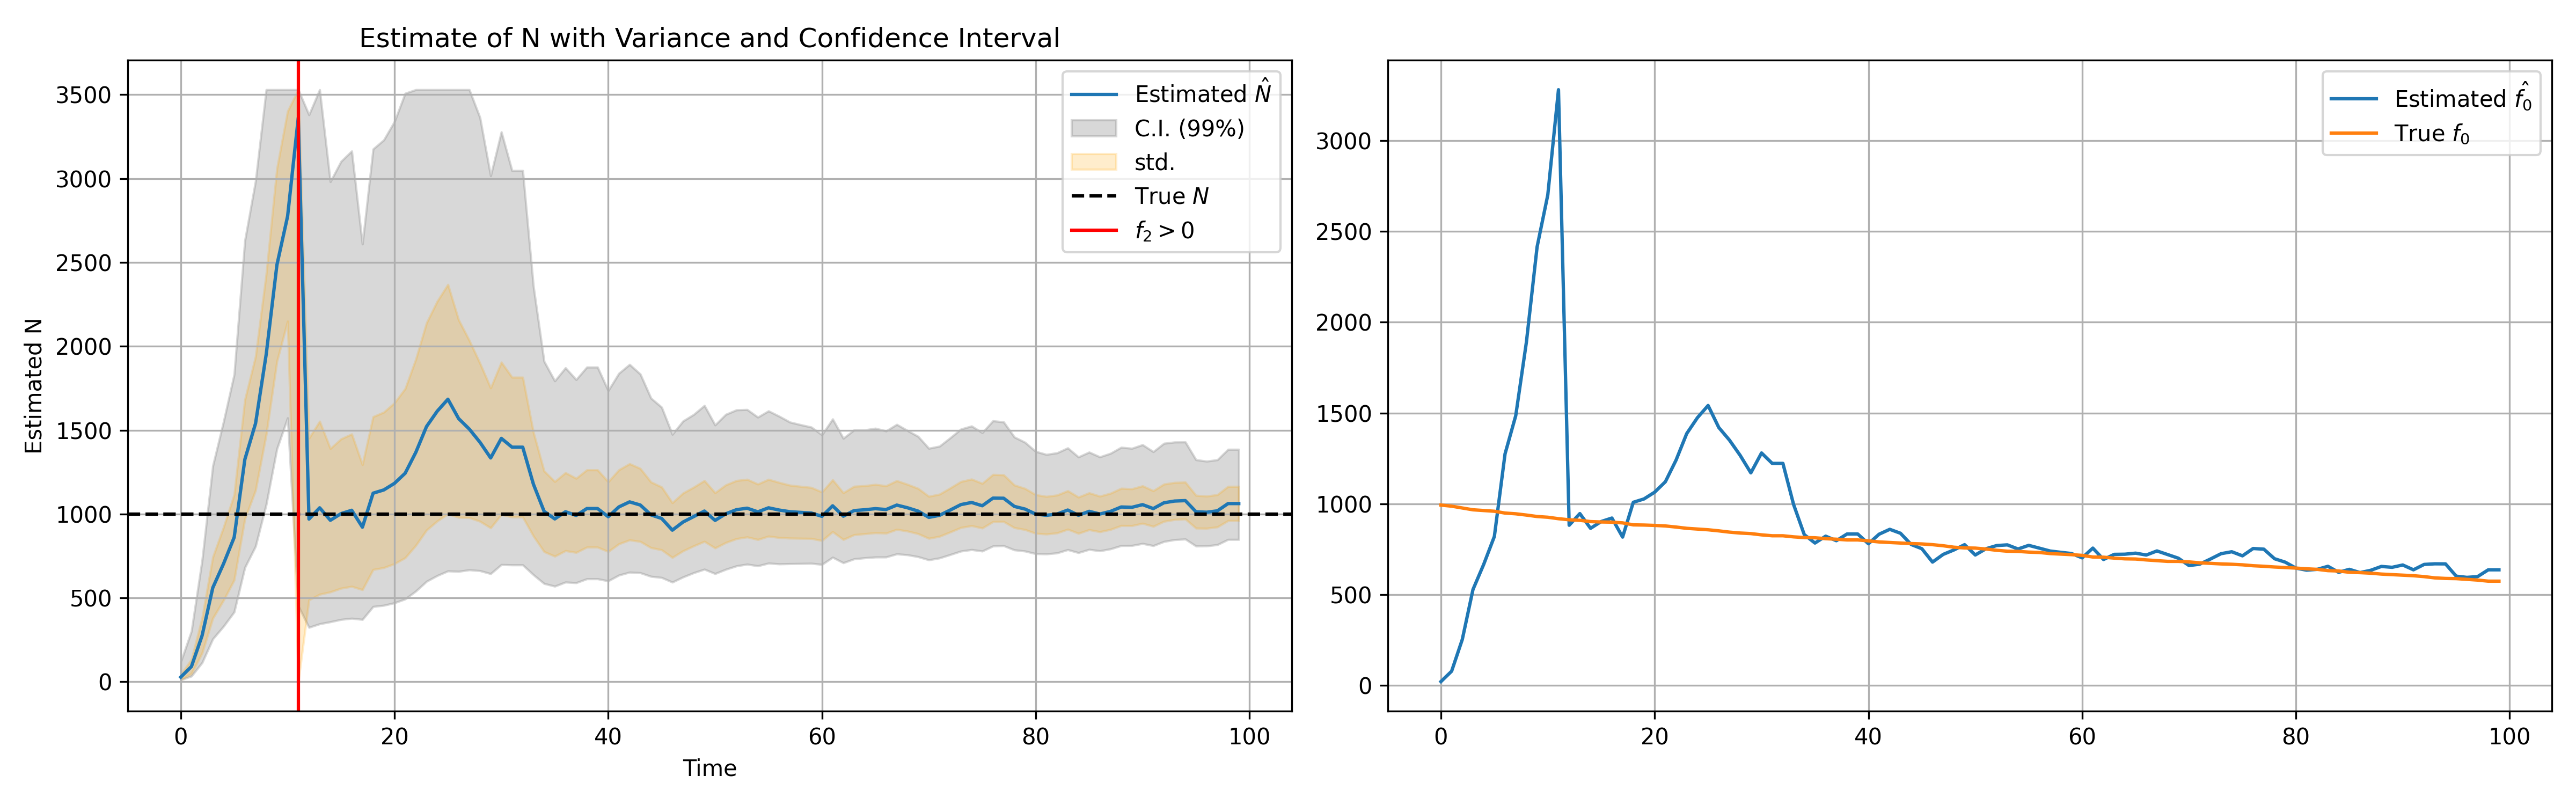
\includegraphics[width=\textwidth]{single_run.png}
    \caption{Single run of the Monte-Carlo simulation for estimating $\hat{N}$ with a true population size of $N=1000$ and a probability distribution of $p_i \sim U(0, 0.01)$.}
    \label{fig:f0_hat_comparison}
\end{figure}



We remark that the behavior observed in Figure~\ref{fig:f0_hat_comparison} is not systematic, as the jump is very extreme. We found this example by chance when plotting the results for a single run. However, it provides us with great insights into the behavior of the estimators.

\begin{center}
    \noindent\rule{0.2\linewidth}{0.4pt}
    \hspace{0.02\linewidth}
    \textbf{End of the core answer of Question 2}
    \hspace{0.02\linewidth}
    \rule{0.2\linewidth}{0.4pt}
\end{center}

While this remaining part relates to the discussion of Problem 2, and can therefore be considered as part of the answer, we understand that only readers interested in the problem formulated in Equation~\ref{eq:goal_equation} will be interested in this section. 
Therefore, if the reader thinks that the explanation stated above is sufficient, we do not force them to read the remaining part.

\textbf{Analytical Analysis --- Over-Estimation of the Population Size.}

In the remaining part of this section, we will investigate analytically whether the over-estimation of the population size is a systematic property of the given estimator.


Formally, we are interested in the following question
\begin{equation}
    \Pr(\hat{N} > N) > \Pr(\hat{N} \leq N)\;.
    \label{eq:goal_equation}
\end{equation}

To this end, we will assume that the estimator is unbiased, i.e., that $\mathbb{E}[\hat{N}] = N$. 
Note that Equation~\ref{eq:goal_equation} is not in contradiction with the unbiasness of the estimator, as the expected value is the value towards which the estimator converges to in the limit of the number of samples. However, for finite samples, even if the estimator has a theoretical mean of $N$, if the distribution of the estimated population size is skewed, it is possible that Equation~\ref{eq:goal_equation} holds. 

% Whether this is the case is beyond the scope of this assignment. Investigating this could be an interesting future work.

Before we start, let us first formally define some notation and defintions of $f_i$ that allows us to derive the probability for $\hat{N} > N$.

Let us denote an animal as $X_i$ with $i\in \{1, \dots, N\}$ and $X_i^t\in \{0, 1\}$ denoting whether the animal $i$ has been caught at time step $t$.
Therefore, we can define 
\begin{equation*}
    X_i = \sum_{t=1}^T X_i^t\;,
\end{equation*}
i.e., the total number of times the animal has been caught after $T$ time steps.

Logically, we have that $X_i^t \sim \mathrm{Bernoulli}(p)$ with $p$ being the probability of being caught at time step $t$. In our setting, $p$ follows a specified probability distribution.

We have that $X_i^t$ are i.i.d.\ w.r.t.\ the time steps $t$ and the animals $i$. These are important assumptions.
From this, it follows that $X_i \sim \mathrm{Binomial}(T, p)$ as we have a sum of $T$ independent Bernoulli variables.

We can now formally define $f_k$ as follows using the following set 
\begin{equation*}
    S_k = \left\{ X_i : i \in \{1, \dots, N\} \mid X_i = k \right\}
\end{equation*}
which contains all the animals that have been caught exactly $k$ times within the $T$ time steps.
Therefore, $f_k$ can be defined as follows:
\begin{equation*}
    f_k = |S_k|\;.
\end{equation*}

Because $f_k$ is a random variable, we can define the probability distribution of $f_k$ w.r.t.\ the number of time steps $t$ as binomial distribution:
\begin{align*}
    \Pr(f_k = n\mid T=t) = \mathrm{Binomial}(N, n, \Pr(X_i = k\mid T=t))\;. \quad n \in \{0, 1, \dots, N\}
\end{align*}

Therefore, we need to compute the probability of an animal being caught exactly $k$ times within the $T$ time steps. We have
\begin{align*}
    \Pr(X_i = k \mid T=t') = \mathrm{Binomial}(t', k, \Pr(X_i^t = 1))
\end{align*}
where $\Pr(X_i^t = 1)$ is the probability of an animal being caught at time step $t$.
Because $X_i^t$ is a binary variable, its expected value is its probability, and we can therefore re-use the expected values for the different given probabilities that we computed earlier (see Equation~\ref{eq:expectation_xi_u01},~\ref{eq:expectation_xi_u02},~\ref{eq:expectation_xi_beta13},~\ref{eq:expectation_xi_beta22}).

% We derive the following proposition, which we will use later. Note that Equation~\ref{} is entirely derived by ChatGPT as I was searching whether there were known results for this property. I could have easily derived it myself, however, I wanted to be sure that it lead somewhere. Note that I added some intermediate steps such that I understand each step fully:
% \begin{align*}
%     n \cdot \binom{N}{n} &= n \frac{N!}{n!(N-n)!} \\
%     &= \frac{N!}{(n-1)!(N - n)!} \\
%     &= N\frac{(N-1)!}{(n-1)!(N-n)!} \\
%     % &= N\frac{(N-1)!}{(n-1)!(N-n-1)!\cdot(N-n)} \stepandtag \label{eq:binomial_property} \\
%     % &= N \frac{(N-1)!}{(n-1)!((N-1)-(n-1))!}
%     % &= N \frac{(N-1)!}{(n-1)!(N-n)!} \\
%     &= N \frac{(N-1)!}{(n-1)!(N-1-n+1)!} \\
%     &= N \frac{(N-1)!}{(n-1)!((N-1)-(n-1))!} \\
%     &= N \binom{N-1}{n-1}
% \end{align*}

We can now compute the expected value for each $f_k$:
{
\allowdisplaybreaks
\begin{align*}
    \mathbb{E}\left[ f_k \mid T=t \right] &= \sum_{n=0}^N n \cdot \Pr(f_k = n \mid T=t) \\
    &= \sum_{n=1}^N n \cdot \mathrm{Binomial}(N, n, \Pr(X_i = k \mid T=t)) \\
    &= \sum_{n=1}^N n \cdot \mathrm{Binomial}(N, n, \mathrm{Binomial}(t, k, p)) 
    % &&p = \mathbb{E}[X_i^t = 1]
    \\
    &= \sum_{n=1}^N n \cdot \mathrm{Binomial}\left( N, n, \binom{t}{k} p^k {(1-p)}^{t-k} \right) \\
    &= \mathbb{E}\left[ \mathrm{Binomial} \left( N, n, \binom{t}{k} p^k {(1-p)}^{t-k} \right) \right] \\
    &= N \cdot \binom{t}{k} p^k {(1-p)}^{t-k}
\end{align*}
}
% We can simplify this further by using the Binomial theorem (also known as Binomial expension).\!\footnote{See \url{https://en.wikipedia.org/wiki/Binomial_theorem}. The idea of using it came from ChatGPT, as I was searching for ways to simplify the expression with the complex power.}

Therefore, we can now compute the expected value for $n$:
\begin{align*}
    \mathbb{E}\left[ n \right] &= \mathbb{E}\left[ \sum_{t=1}^T f_k \right] \\
    &= \sum_{k=1}^T \mathbb{E}\left[ f_k \right] \\
    &= \sum_{k=1}^T \mathbb{E}\left[ f_k \mid T=T\right] \\
    % &= \sum_{k=1}^T \mathbb{E}\left[ f_k \mid T=T\right] \\
    &= \sum_{k=1}^T N \cdot \binom{t}{k} p^k {(1-p)}^{T-k} \\
    &= N \cdot \sum_{k=1}^T \binom{t}{k} p^k {(1-p)}^{T-k} \\
    &= N \cdot \left[ \left( \sum_{k=0}^T \binom{t}{k} p^k {(1-p)}^{T-k} \right) - \binom{t}{0} p^0 {(1-p)}^{T-0}  \right] \\
    &= N \cdot \left[ 1 - 1{(1-p)}^{T} \right]  \\
    &= N \cdot \left( 1 - {(1-p)}^T \right) \stepandtag \label{eq:expected_value_n}\;.
\end{align*}
We report on the expected values for $n$ with $T=40$ for our four probability distributions in Table~\ref{tab:expected_value_n}.
\begin{table}[t]
    \centering
    \begin{tabular}{c|c c c}
        \toprule
         & \multicolumn{3}{c}{Expected Value for $n$} \\
        \midrule
        $N$ & $500$ & $1000$ & $5000$ \\
        \midrule
        $U(0, 0.01)$ & $90.83$ & $181.67$ & $908.39$\\
        $U(0, 0.02)$ & $165.51$ & $331.02$ & $1655.14$\\
    \end{tabular}
    \caption{Expected value for $n$ for $T=40$ and $N \in \{500, 1000, 5000\}$ for the different probability distributions.}
    \label{tab:expected_value_n}
\end{table}
Note that Equation~\ref{eq:expected_value_n} is equal to 
\begin{align*}
    \mathbb{E}\left[ n \right] &= N \cdot \left( 1 - {(1-p)}^T \right) \\
    &= N \cdot \left( 1 - \binom{T}{0} p^0 (1-p)^T \right) \\
    &= N - N \cdot \binom{T}{0} p^0 (1-p)^T \\
    &= N - \mathbb{E}\left[ f_0 \mid T=T \right] 
\end{align*}
which is exactly what we would expect.
% Let us now compute the skewness of the distribution of $n$. 
% Because we know that $f_k$ follows a binomial distribution, we can compute 

Because $\hat{N} = n + \hat{f_0}$, we now compute the expected value for $\hat{f_0}$.
As $\hat{f_0}$ is conditional on whether $f_2 \neq 0$ or $f_2 = 0$, we need to compute the probability of $f_2 = 0$ and $f_2 \neq 0$.
% Note that we assume that $f_2 \neq 0$, as otherwise we would need to marginalize over the probability of $f_2 = 0$. Given that we have $T \gg 0$, we expect the probability of $f_2 = 0$ to be extremely small, and therefore negligable.
% Nevertheless, we can easily compute the probability of $f_2 = 0$:
Because we model $f_k$ as a binomial distribution, we can easily compute the probability of $\Pr(f_2 = 0)$. We have 
\begin{align*}
    \Pr(f_2 = 0 \mid T=T) &= \mathrm{Binomial}(N, 0, \Pr(X_i = 2\mid T=T)) \\
    &= (1 - \Pr(X_i = 2\mid T=T))^N \\
    &= {\left( 1 - \mathrm{Binomial}(T, 2, p) \right)}^N\;.
\end{align*}
We report on the probabilities for our four probability distributions for $p$ in Table~\ref{tab:probability_f2_eq_0}. We also plot the probability changing over time in Figure~\ref{fig:probability_f2_eq_0_over_time}.

\begin{table}[t]
    \centering
    \begin{tabular}{c|c c c}
        \toprule
         & \multicolumn{3}{c}{$\Pr(f_2 = 0 \mid T=40)$} \\
        \midrule
        $N$ & $500$ & $1000$ & $5000$ \\
        \midrule
        $p=0.01$ & $1.3 \times 10^{-12}$ & $1.7 \times 10^{-24}$ & $1.6 \times 10^{-119}$ \\
        $p=0.005$ & $2.96 \times 10^{-4}$ & $8.77 \times 10^{-8}$ & $5.19 \times 10^{-36}$ \\
        % \bottomrule
    \end{tabular}
    \caption{Probability for $f_2 = 0$ $n$ for $T=40$ and $N \in \{500, 1000, 5000\}$ for the different probability distributions.}
    \label{tab:probability_f2_eq_0}
\end{table}




Before investigating the case where $f_2\neq 0$, let us first investigate the bias of $\hat{f_0}\mid f_2 = 0$.
We have 
{
\allowdisplaybreaks
\begin{align*}
    \mathbb{E}\left[ \hat{f_0} \mid f_2 = 0, T=t \right] &= \mathbb{E}\left[ \frac{f_1^2 - f_1}{2} \right] \\ 
    &= \sum_{n=0}^N \frac{n^2 - n}{2} \cdot \Pr(f_1 = n \mid T=t) \\
    &= \sum_{n=0}^N \frac{n^2 - n}{2} \cdot \mathrm{Binomial}(N, n, \Pr(X_i = 1 \mid T=t)) \\
    &= \sum_{n=0}^N \frac{n^2 - n}{2} \cdot \mathrm{Binomial}(N, n, \mathrm{Binomial}(t, 1, p)) \\
    &= \sum_{n=0}^N \frac{n^2 - n}{2} \cdot \mathrm{Binomial}(N, n, \binom{t}{1} p^1 {(1-p)}^{t-1})
    % &= \sum_{n=0}^N \frac{n^2 - n}{2} \cdot \binom{N}{n} {\left( \binom{t}{1} p^1 {(1-p)}^{t-1} \right)}^{n} {\left( 1 - \binom{t}{1} p^1 {(1-p)}^{t-1} \right)}^{N-n} \\
    % &= \sum_{n=0}^N \frac{n^2 - n}{2} \cdot \binom{N}{n} {\binom{t}{1}}^n p^n {(1-p)}^{(t-1)\cdot n} {\left( 1 - \binom{t}{1} p^1 {(1-p)}^{t-1} \right)}^{N-n} \\
\end{align*}
which we we cannot simplify further (at least such that is gives us more insights). We use python to compute the expected value for $\hat{f_0} \mid f_2 = 0, T=40$ for our four probability distributions and report on the results in Table~\ref{tab:expected_value_f0_f2_eq_0}. While the expected values for $\hat{f_0}\mid f_2 = 0$ are very large, it is easy to see that when multiplied with the probability of $f_2 = 0$, we would get values that are almost zero. The interested reader can find a plot describing the rescaled expected value in Figure~\ref{fig:expectation_f0_f2_eq_0_rescaled} in the Appendix.


\begin{table}[t]
    \centering
    \begin{tabular}{c|c c c}
        \toprule
         & \multicolumn{3}{c}{$\mathbb{E}[\hat{f_0} \mid f_2 = 0, T=40]$} \\
        \midrule
        $N$ & $500$ & $1000$ & $5000$ \\
        \midrule
        $p=0.01$  & $9113.93$   & $36492.25$  & $913036.85$ \\
        $p=0.005$ & $3375.21$   & $13514.37$  & $338129.79$ \\
        % \bottomrule
    \end{tabular}
    \caption{Expected value for $\hat{f_0}$ conditioned on $f_2 = 0$ for $T=40$ and $N \in \{500, 1000, 5000\}$ for different values of $p$.}
    \label{tab:expected_value_f0_f2_eq_0}
\end{table}
}

Let us now investigate the bias of $\hat{f_0}$ when $f_2 \neq 0$. As $\hat{f_0}$ is defined as a function of $f_1$ and $f_2$, and that both of them are dependent,\!\footnote{We attach in the Appendix (See Section~\ref{sec:proof_dependency_f1_f2}) a proof of the dependency of $f_1$ and $f_2$ generated by ChatGPT.  As the proof is not critical for the continuation of this derivation, we add it to the Appendix for the interested reader. Note that while we have deleted the exact output of ChatGPT, the idea of this proof is still to be credited to ChatGPT.} we have to model their probability jointly for a fully analytical derivation.
While it is very tempting to add a independence assumption on the distributions of $f_1$ and $f_2$, their correlation is too strong to be ignored, and the obtained results are not meaningful.\!\footnote{This was our first attempt. However, our formula estimated $\mathbb{E}[\hat{f_0}\mid f_2 > 0, T=40]$ to be almost zero for all probability distributions and sample sizes.}
% However, as modeling the joint probability is very complex, we resort to an approximation by introducing an assumption that doesn't hold.
% Therefore, for ease of computability, we will assume that $f_1$ and $f_2$ are independent. Note that their correlation is not zero, and can be meaningful for larger catching probabilities $p$. 
We show the correlations for our probability distributions in Table~\ref{tab:correlation_f1_f2} in the Appendix.

% We can now compute the expected value of $\hat{f_0}\mid f_2 > 0$ as follows:
% {
% \allowdisplaybreaks
% \begin{align*}
%     \mathbb{E}[\hat{f_0}\mid f_2 > 0] &= \mathbb{E}\left[ \frac{f_1^2}{2 f_2} \mid f_2 > 0 \right] \\
%     &= \sum_{n=0}^{N-1} \sum_{m=1}^{N-n} \frac{n^2}{2 m} \cdot \Pr(f_1 = n \mid T=t) \cdot \Pr(f_2 = m \mid T=t) \stepandtag \label{eq:expectation_f0_f2_gt_0}
%     % &= \sum_{n=0}^{N-1} \sum_{m=1}^{N-n} \frac{n^2}{2 m} \cdot \Pr(f_1 = n \mid T=t) \cdot \Pr(f_2 = m \mid T=t) \stepandtag \label{eq:expectation_f0_f2_gt_0}
%     % &= \sum_{n=0}^{N-1} \sum_{m=1}^{N-n} \frac{n^2}{2 m} \cdot \Pr(f_1 = n \mid T=t) \cdot \Pr(f_2 = m \mid T=t) \\
% \end{align*}
% which we could simplify further, however, we believe that we would not gain a relationship to $f_0$ by doing so. Therefore, we resort to modeling the expectation from Equation~\ref{eq:expectation_f0_f2_gt_0} using Python. 
% }

The only way to compute $\mathbb{E}[\hat{f_0}\mid f_2 > 0]$ is by marginalizing over all possible values for all $f_i$ with $f_i \notin \{1, 2\}$, i.e.,
\begin{align*}
    \mathbb{E}[\hat{f_0}\mid f_2 > 0] &= \mathbb{E}\left[ \frac{f_1^2}{2 f_2} \mid f_2 > 0 \right] \\
    &= \sum_{n=0}^{N-1} \sum_{m=1}^{N-n} \frac{n^2}{2 m} \cdot \Pr(f_1 = n, f_2 = m \mid T=t) \\
    &= \sum_{n=0}^{N-1} \sum_{m=1}^{N-n} \frac{n^2}{2 m} \cdot \left( \sum_{k_3 = 0}^{N-n-m} \cdots \sum_{k_N = 0}^{N-n-m-\sum_{i=3}^{N}k_i} \Pr(f_1 = n, f_2 = m, f_3 = k_3, \dots, f_N=k_N \mid T=t) \right) \stepandtag \label{eq:expectation_f0_f2_gt_0_marginalized}
\end{align*}
which is computationally infeasible. Furthermore, we cannot simplify Equation~\ref{eq:expectation_f0_f2_gt_0_marginalized} , as every $f_i$ is dependent on each $f_j$ with $i\neq j$. Note that especially for our simulation size, using $N=5000$ would result in a value proportional to $2^{5000}$, which is a number with 1506 digits.

Therefore, without further assumptions, we are unsure whether we can show that $N$ is unbiased --- let alone skewed --- in a fully analytical way.

Nevertheless, as we can model individual $f_i$ using a binomial distribution, we can model the skewness of both $f_1$ and $f_2$ analytically. This might give us some insights into whether Equation~\ref{eq:goal_equation} holds.


\textbf{Skewness}

Let us now investigate the skewness of $f_i \sim \mathrm{Binomial}(T, p_i)$. 
It is a well known fact that the skewness of a binomial distribution is given by 
\begin{equation*}
    \mathrm{Skewness}(f_i) = \frac{(1-p) - p}{\sqrt{N \cdot p \cdot (1-p)}}\;.
\end{equation*}

For $f_1$, we have that 
\begin{align*}
    \mathrm{Skewness}(f_1) &= \frac{(1 - \Pr(X_i = 1 \mid T=T)) - \Pr(X_i = 1 \mid T=T)}{\sqrt{N \cdot \Pr(X_i = 1 \mid T=T) \cdot (1 - \Pr(X_i = 1 \mid T=T))}} \\
    &= \frac{\left( 1 - \binom{T}{1} p^1 {(1-p)}^{T-1} \right) - \binom{T}{1} p^1 {(1-p)}^{T-1}}{\sqrt{
        N \cdot \left( 1 - \binom{T}{1} p^1 {(1-p)}^{T-1} \right) \cdot \binom{T}{1} p^1 {(1-p)}^{T-1}
    }} \\
    &= \frac{ 1 - 2 \cdot \binom{T}{1} p^1 {(1-p)}^{T-1}}{\sqrt{
        N \cdot \left( 1 - \binom{T}{1} p^1 {(1-p)}^{T-1} \right) \cdot \binom{T}{1} p^1 {(1-p)}^{T-1}
    }} 
\end{align*}
which we will compute using python. This results in the results shown in Table~\ref{tab:skewness_f1_f2}.


\begin{table}[tbp]
    \centering
    \begin{tabular}{c|c c c| c c c}
        \toprule
         & \multicolumn{3}{c}{$\mathrm{Skewness}(f_1)$} & \multicolumn{3}{c}{$\mathrm{Skewness}(f_2)$} \\
        \midrule
        $N$ & $500$ & $1000$ & $5000$ & $500$ & $1000$ & $5000$ \\
        \midrule
        $p=0.01$  & $0.0463$   & $0.0327$  & $0.0146$ & $0.17799$ & $0.12585$ & $0.05628$ \\
        $p=0.005$ & $0.0809$   & $0.0572$  & $0.0256$ & $0.34368$ & $0.24302$ & $0.10868$ \\
        % \bottomrule
    \end{tabular}
    \caption{Skewness for $f_1$ and $f_2$ for $T=40$ when modeled as a binomial distribution.}
    \label{tab:skewness_f1_f2}
\end{table}

Recall that a positive value for skewness indicates that the distribution has a median and mode on the left of the mean, and therefore the majority of the values are on the left, and the distribution is tailed to the right. A negative value has the same interpretation, but flipped. We added a visualization of the interpretation of the value of skewness in Figure~\ref{fig:interpretation_skewness} in the Appendix.

From Table~\ref{tab:skewness_f1_f2}, it is easy to see that all values are positive. Therefore, we know that $f_1$ and $f_2$ have the majority of their values to the left of the mean, i.e., have a lower value than the mean.
Naturally, the more samples we have, the less skewed the distribution is, this is also reflected in the table.

We are unable to compute the skewness of $n$, which follows the same argument as above, namely that all the $f_i$ are dependent on each other. While all the $f_i$ can be modeled using a multinomial distribution, a closed form solution to the skewness of a multinomial distribution is unknown to us, we couldn't find any literature on the topic.
% This could be an interesting topic for future research --- assuming that it is even possible.
Therefore, we assume that $n$ is either not skewed, or very lightly skewed in the oposite direction of $\hat{f_0}$. Otherwise, our argument does not hold.

However, and this is very interesting, we can say something about the skewness of $\hat{f_0}$.
When looking at the skewness of $\hat{f_0}$ in Table~\ref{tab:skewness_f1_f2}, we see that $f_1$ is less skewed than $f_2$. In fact, $f_2$ is skewed around 4--5 times more than $f_1$.
This is a very important and interesting observation. 

This shows that, for small and finite samples, we are more likely to sample values for $f_1$ and $f_2$ below the mean than above. The inequality in the skewness from Table~\ref{tab:skewness_f1_f2} indicates that, $f_2$ is sampled more below the expected value of $f_2$ than compared to $f_1$.

As we divide the less undersampled value by the more undersampled value, we argue that $\hat{f_0}$ is negatively skewed. This follows from the argument that, assuming that $\mathbb{E}[\hat{f_0}] = f_0$ holds, we would $\frac{f_1}{f_2} \approx 5$, which would mean that we overestimate $f_0$.\!\footnote{We have not used skewness in any work before. Therefore, we are unsure if this is correct. However, that this ration is larger than 1 is what we are trying to argue.}
As we are squaring the $f_1$ value, and only increasing the value of $f_2$ linearly in $\hat{f_0}$, we believe that this reduces the extremeness of the skewness of $\hat{f_0}$ significantly.

Therefore, assuming that $\mathbb{E}\left[ \hat{f_0} \right] = f_0$ holds, we argue that Equation~\ref{eq:goal_equation} holds.
How to prove this formally is unknown to us; We believe that this statement is not true in general --- as in the limit, the skewness, variance, and bias becomes zero --- but we argue that especially for small finite samples, the statement holds.

We tried to get some help from ChatGPT, as we hope that it can uncover some theorems unknown to us. While it gave us a negative answer on whether the statement holds, it said that if if our distribution is log-concave, then $P(X < E[X]) \geq \frac{1}{2}$ holds for some random variable $X \sim G$ with $G$ being a log-concave positively skewed distribution.
As the Binomial distribution is log-concave,\!\footnote{See \url{https://en.wikipedia.org/wiki/Logarithmically_concave_function}. We are unsure if this is correct for all cases, especially ours.}, we \textit{could} argue that because we hypothesize that $\frac{f_1^2}{2f_2}$ is negatively skewed, we have $P(\hat{f_0} > f_0) \geq \frac{1}{2}\Rightarrow P(\hat{f_0} > f_0) > P(\hat{f_0} \leq f_0)$. But as we are unsure about the correctness of our argument, we will only mention it here.

% This unequality in the skewness means that, when sampling for values of $f_1$ during our simulations, we are 

\pagebreak

\chapter{Part B: Data Analysis}

\section{Data pre-processing and experimental setup}

We combined two Equinox datasets containing change metrics and CK/OO metrics and used the class identifier \texttt{classname} as the join key. Defect-related metadata columns were removed from the feature set, while \texttt{bugs} was retained as the target variable.

We merged the two datasets using a one-to-one inner join on \texttt{classname}. After merging, all feature columns, as well as the target, were converted to numeric values. The final dataset contains \textbf{324 classes}, \textbf{32 features}, and one target variable.

The dataset was split into a training set (67\%) and a test set (33\%). To preserve the distribution of bug counts, we used stratified random sampling based on the predefined bug-count bins (0, 1--2, 3--5, 6+). The stratification variable was used only for splitting and removed afterwards.

The resulting training and test sets were saved and used consistently in all analyses. Models were selected on the training set and the final selected model was evaluated on the test set.

\subsection{Data Analysis}

Before training our Poisson and logistic regression models, we first investigate the distribution of the data.

As a first step, we plot the histogram of the 32 features that we use in Figure~\ref{fig:feature_histogram_raw}. While we only display the marginal distributions of the features, and therefore omit the joint interaction between multiple features, plotting the joint interaction would require 512 plots, which, for the scope of this task, is too much to look at.

Figure~\ref{fig:feature_histogram_raw} clearly shows that most of the data are not only skewed to the left, i.e., have most of their value close to zero with heavy tails containing high values, but we also remark that the range of certain variables is extremely large (e.g. \texttt{numberOfLinesOfCode} which spans the range of around 0--1500).

% To counteract this effect, we propose to first transform the data 

While the skewness of the response variable is not an issue, as we use Poisson regression, which can handle skewed data, and logistic regression for the binary case, we argue that the skewness in the features might impact the model negatively.
Therefore, we propose to transform the 32 features into the log-domain, which should reduce the effect of the skewness.

Finally, to make the training of the models easier, we normalize every feature such that they have a mean of zero and a standard deviation of 1. While this hinders slightly the interpretation of the learned parameter $\beta$, we remark that by using the inverse of the normalization used on the features, we can give meaning to the learned parameters again.

We plot the distribution of the log-transformed and normalized features in Figure~\ref{fig:feature_histogram_log_transformed}. While we observe that many features remain skewed to the left, we also observe that the values of the features are more evenly distributed, with many features almost containing a gaussian bell shape (e.g. \texttt{avgCodeChrunUntil}). 

\begin{figure}[t]
    \centering
    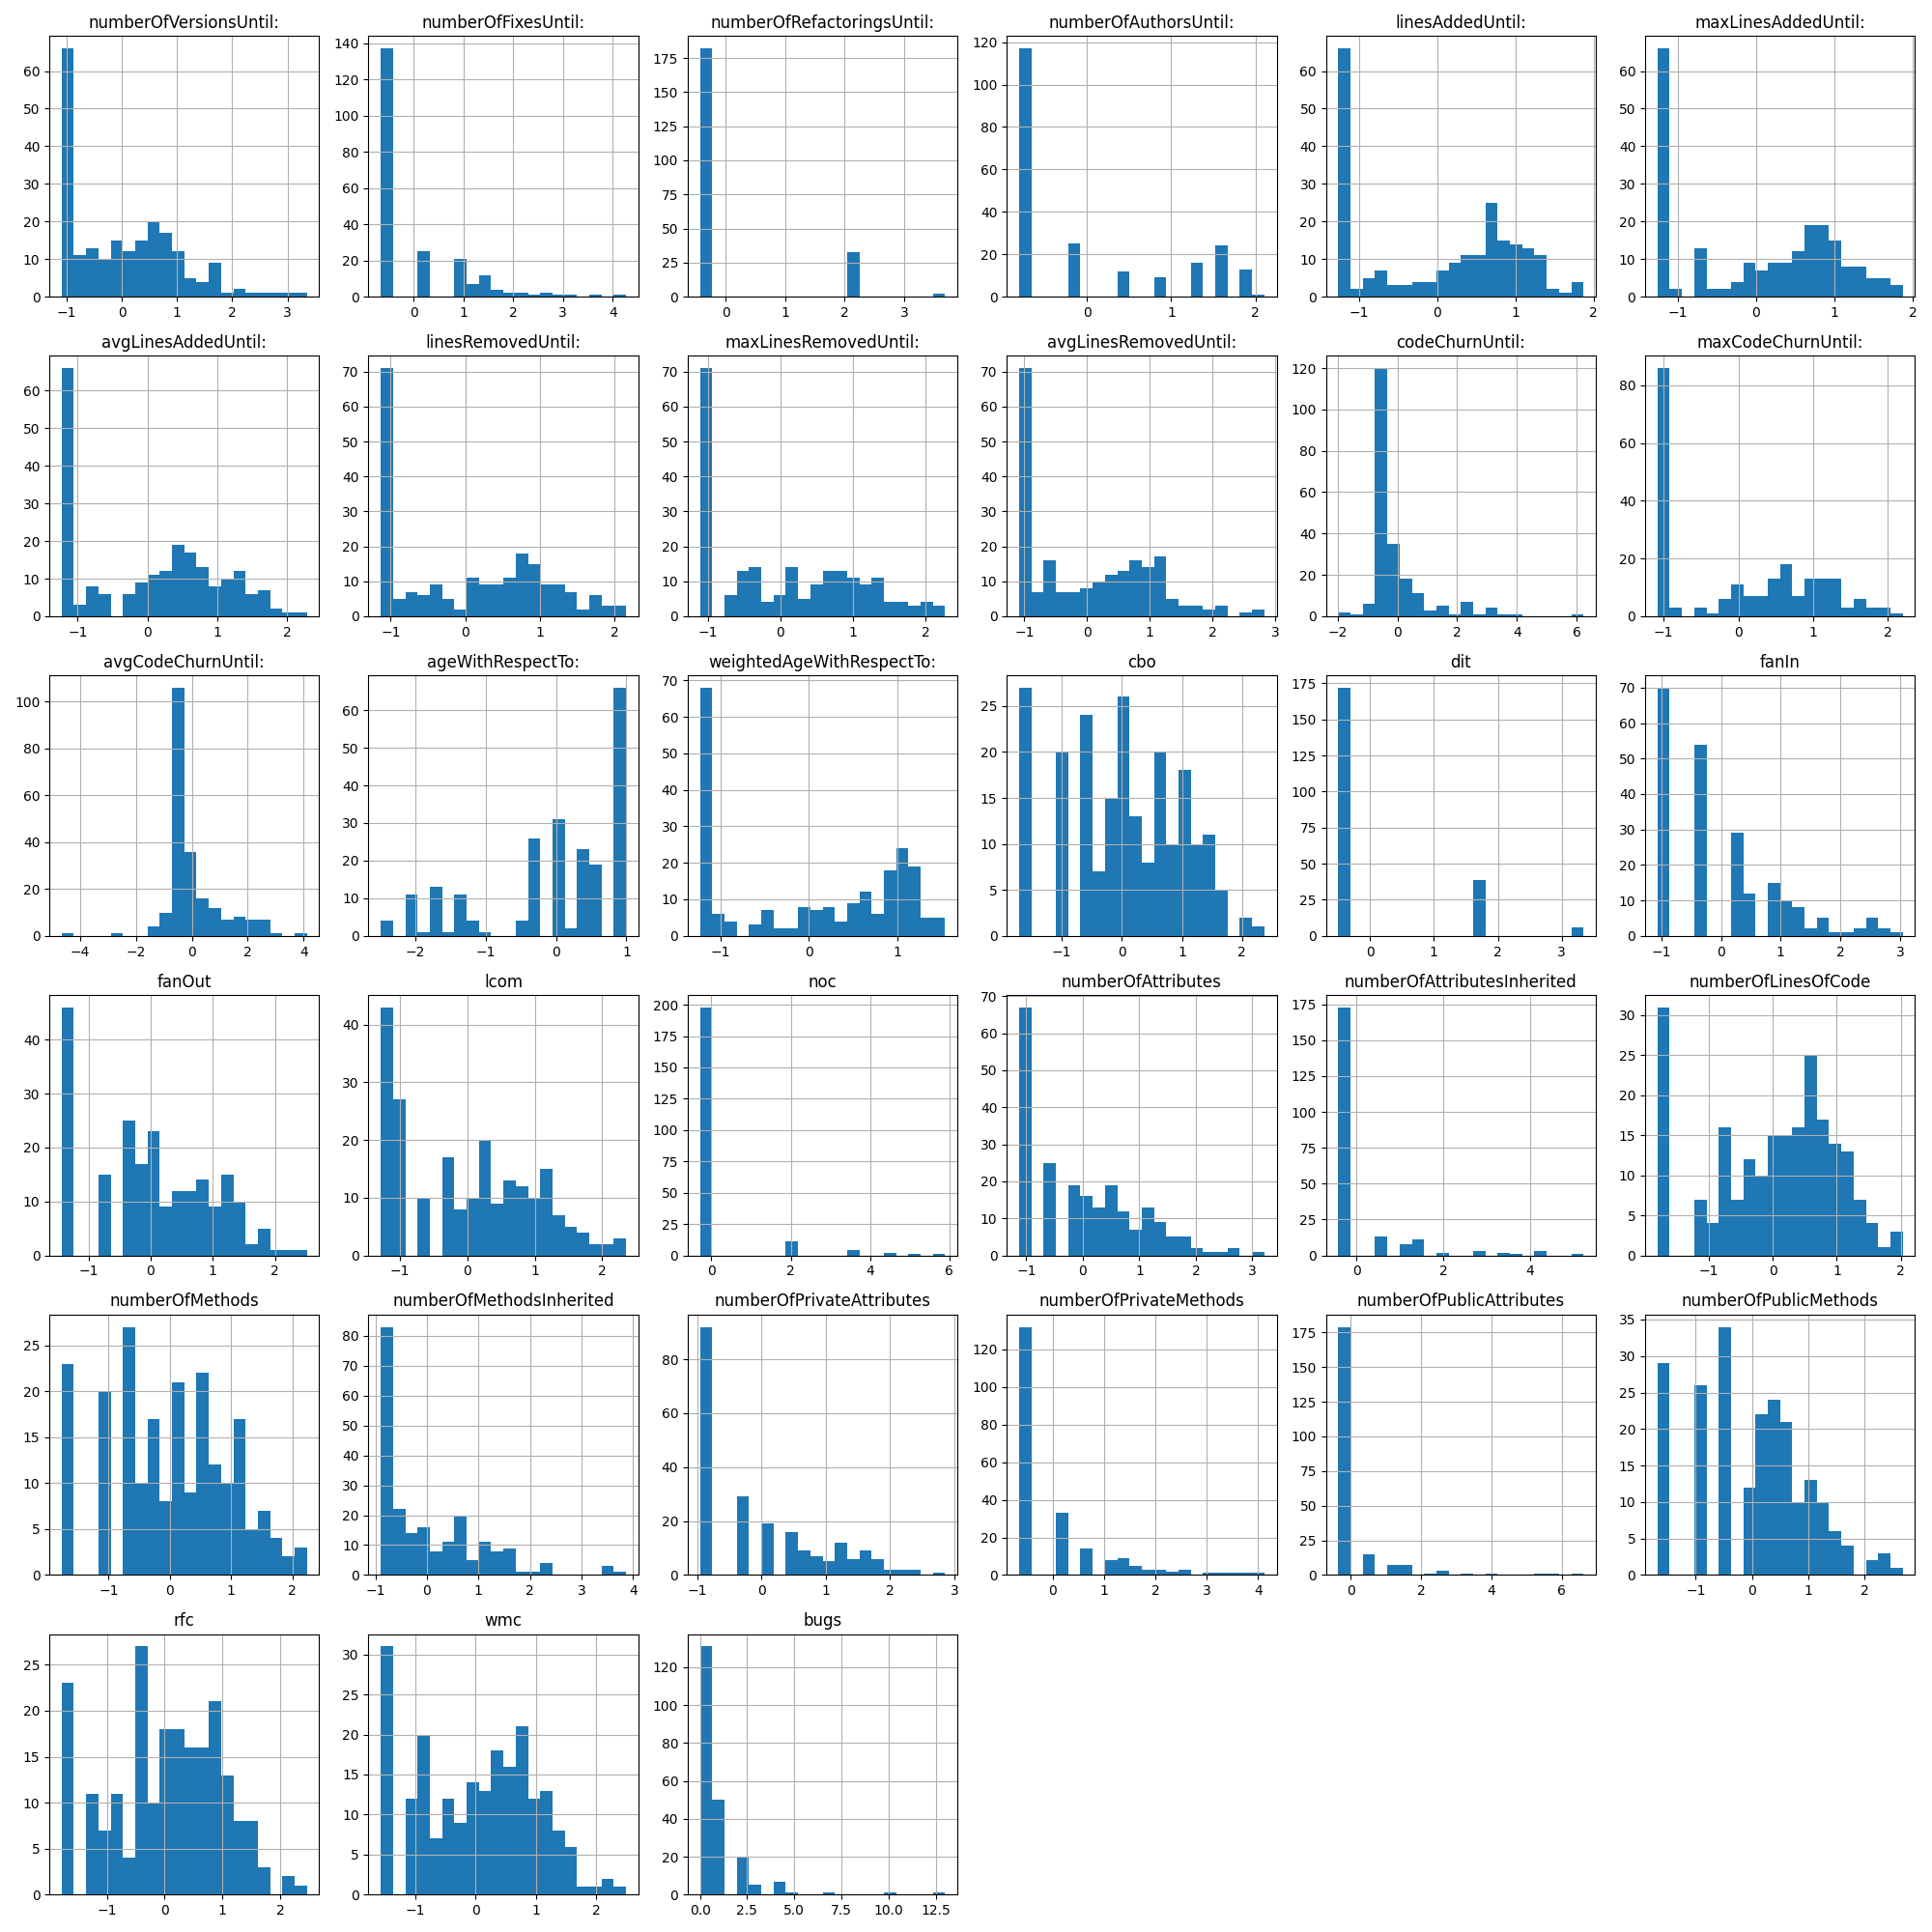
\includegraphics[width=0.75\linewidth]{extra_plots/raw_feature_histograms_log_and_normalized.png}
    \caption{Histograms of the 32 features after transforming them into the log domain and normalizing them.}
    \label{fig:feature_histogram_log_transformed}
\end{figure}

As the log-transformation might have destroyed the (linear) relationship of certain variables --- especially if it is with the response variable --- we will compare performance of the log-transformed and normalized data to the just normalized data.

Note that to ensure a valid log-transformation, we added a constant to each of the features, to ensure that each feature is greater than zero. This is part of our log-transform step.

\section{Poisson regression}

\subsection{Stepwise model selection}
\label{sec:poisson_stepwise}
We use Poisson regression to model the number of bugs for each function.
To find the best set of features to use for the Poisson regression,
% Since the response variable is count data, a generalized linear model with Poisson family and log link was used. 
we performed model selection using both forward and backward stepwise selection, starting from a model with only an intercept.

To find the best model from the training features alone, we scored each found model using both AIC and BIC, as we are also interested in understanding when one is better than the other.

\begin{figure}[t]
    \centering
    {\textbf{Normalized} Data} \\
    \subfloat[Using \textbf{AIC}.]{
        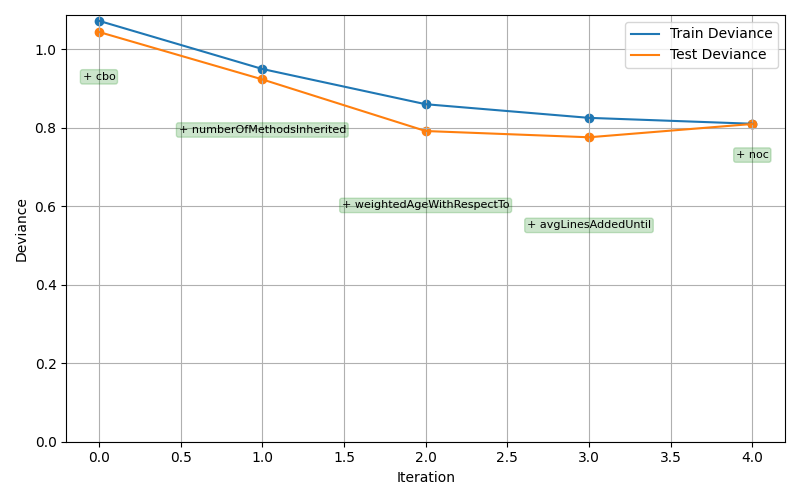
\includegraphics[width=0.45\linewidth]{extra_plots/poisson_regression_stepwise_deviance_history_aic.png}
    }
    \hfill
    \subfloat[Using \textbf{BIC}.]{
        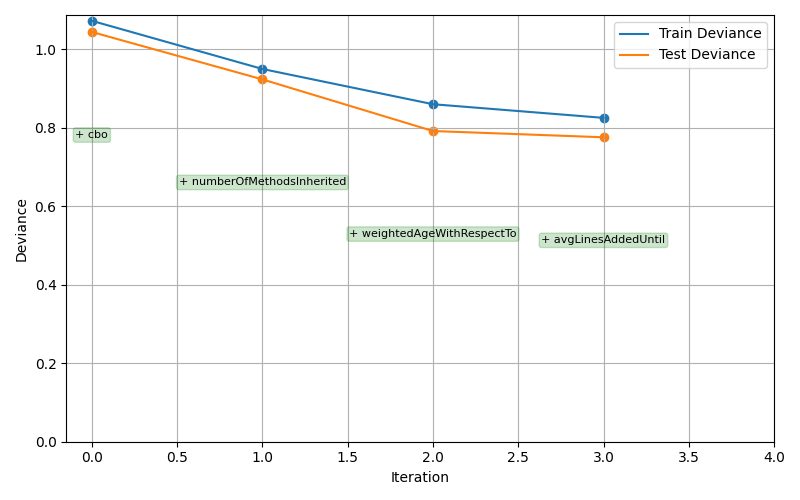
\includegraphics[width=0.45\linewidth]{extra_plots/poisson_regression_stepwise_deviance_history_bic.png}
    }
    \caption{Train and test deviance of the Poisson regression when using stepwise model selection when using the normalized featured. Note that the green boxes starts with + denote which feature has been added to the model.}
    \label{fig:deviance_normalized}
\end{figure}


\begin{figure}[t]
    \centering
    {\textbf{Log-transformed \& Normalized} Data} \\
    \subfloat[Using \textbf{AIC}.]{
        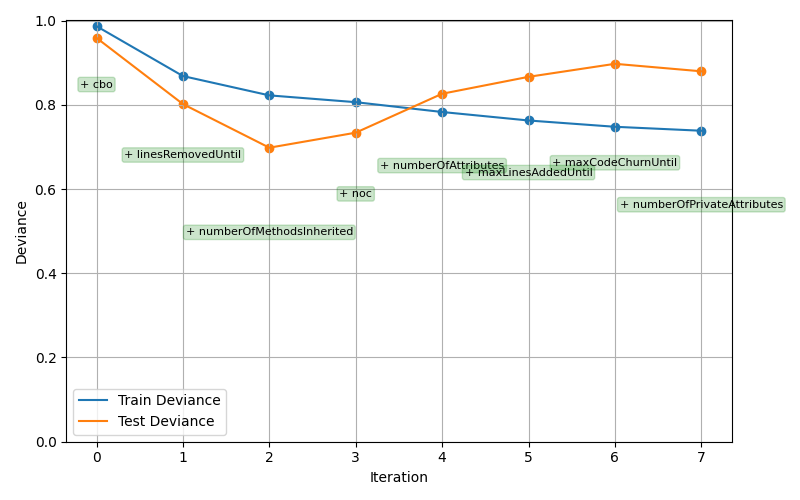
\includegraphics[width=0.45\linewidth]{extra_plots/poisson_regression_stepwise_deviance_history_aic_log.png}
    }
    \hfill
    \subfloat[Using \textbf{BIC}.]{
        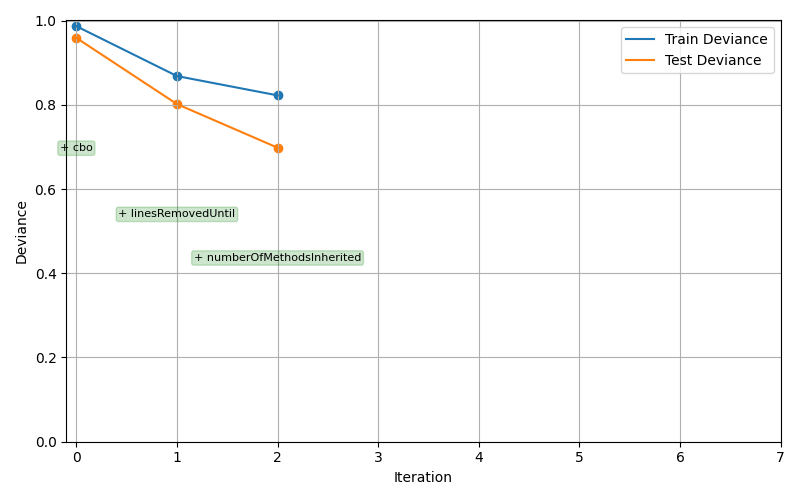
\includegraphics[width=0.45\linewidth]{extra_plots/poisson_regression_stepwise_deviance_history_bic_log.png}
    }
    \caption{Train and test deviance of the Poisson regression when using stepwise model selection when using the log-transformed and normalized featured. Note that the green boxes starts with + denote which feature has been added to the model.}
    \label{fig:deviance_log_transformed_and_normalized}
    % \label{stepwise vs LASSO}
\end{figure}


\textbf{Normalized Data.}
Let us first look at the results from the Poisson regression models found using stepwise model selection. 
In Figure~\ref{fig:deviance_normalized}, we have plotted the train and test poisson-deviation at each step, while using the AIC and BIC scores to estimate when to stop the search. We report on the final mean Poisson deviance in Table~\ref{tab:mean_poisson_deviation_poisson_regression_step_search}.

First, when using AIC, we find a model using 5 features, namely \texttt{cbo}, \texttt{numberOfMethodsInherited}, \\\texttt{weightedAgeWithRespectTo}, \texttt{avgLinesAddedUntil}, and \texttt{noc}.
Interestingly, while the Poisson deviance decreases with each feature that is being added, we observe that adding the \texttt{noc} features makes the test deviance increase, while the train deviance decreases.
This is a sign of overfitting.

Interestingly, when using BIC to score the models, we observe that the same features are being added in the same order. However, when adding a fifth feature, including \texttt{noc}, the BIC score increases, and therefore the search stops. 

\textbf{Log-Transformed and Normalized Data.}
We run the same code on the data we transformed to the log space. We plot the train and test mean Poisson deviance in Figure~\ref{fig:deviance_log_transformed_and_normalized} and report on the final mean Poisson deviance in Table~\ref{tab:mean_poisson_deviation_poisson_regression_step_search}.

First, we remark that, compared to the normalized data, using AIC for scoring the search finds 7 features, whereas when using BIC, only 3 features are found.

Similarly as for the just normalized data, BIC stops the search as soon as the Poisson deviance of the test set increases, while finding the same sets of features.

Interestingly, we remark that first transforming the data to the log domain uncovers new relationships. This can be seen from the first model from both Figure~\ref{fig:deviance_normalized} and Figure~\ref{fig:deviance_log_transformed_and_normalized}, which only consists of the \texttt{cbo} feature and an intercept. 
Whereas for the just normalized data, the train and test deviance is above 1, when using the log-transformed data, the mean Poisson deviance is bellow 1 for both the train and test set.

This clearly shows that transforming the features to the log space allows the linear relationship to explain more of the variance, and therefore have better predictions.


% Train deviance: 0.8256935176391517
% Test deviance: 0.7761751965293804
% Train deviance: 0.7383483742906413
% Test deviance: 0.8794590092835627
% Train deviance: 0.8223124733984547
% Test deviance: 0.6980782248498346
\begin{table}[tbp]
    \centering
    \begin{tabular}{ll|cc}
         \toprule
         Search Score & Dataset & Train Deviation ($\downarrow$) & Test ($\downarrow$)  \\
         % \toprule
         \midrule
         \multirow{2}{*}{AIC} & Normalized & $0.81064$ & $0.81010$ \\
         &Log-Transformed \& Normalized & $\textbf{0.73834}$ & $0.87946$ \\
         \midrule
         \multirow{2}{*}{BIC} & Normalized & $ 0.82569$ & $0.77617$ \\
         &Log-Transformed \& Normalized & ${0.82231}$ & $\mathbf{0.69807}$ \\
         \bottomrule
    \end{tabular}
    \caption{The mean Poisson deviation values for the best \textbf{Poisson regression model} obtained using \textbf{Stepwise model search} for the different datasets. We highlight in bold the best value of the table for each of the data splits.}
    \label{tab:mean_poisson_deviation_poisson_regression_step_search}
\end{table}


\textbf{Analysis of the Parameters.}
Before looking at the Logistic regression, let us first investigate the values of the found parameters.
From the lecture, we know that increasing the features of a sample $x\in \mathbb{R}^D$ by $\delta\in\mathbb{R}^D$ results in
\begin{equation}
    \frac{\mathbb{E}[y\mid x+\delta]}{\mathbb{E}[y\mid x]} = \exp(\beta \cdot \delta)\;. 
    \label{eq:increase_parameter}
\end{equation}
We can easily understand the impact of each parameter on the prediction by constructing $\delta$ as follows: Let us investigate the increase of the raw feature by one unit. We can construct such a $\delta_i$ for each feature as follows:
\begin{equation*}
    \delta_i = \frac{1}{\sigma_i}
\end{equation*}
as we have 
{
\allowdisplaybreaks
\begin{align*}
    \mathrm{Normalized}(x) + \delta_i &= \frac{x-\mu}{\sigma} + (0, \dots, \underbrace{\frac{1}{\sigma_i}}_i, \dots, 0) \\
    &= \frac{x-\mu}{\sigma} + \frac{1}{\sigma}(0, \dots, \underbrace{1}_i, \dots, 0) \\
    &= \frac{x-\mu}{\sigma} + \frac{1}{\sigma}\delta \\
    &= \frac{x -\mu + \delta}{\sigma} \\
    &= \mathrm{Normalize}(x+\delta)
\end{align*}
}
with $\delta$ denoting a one hot vector at the index of the feature of interest.

It is important to note that we are unable to perform such a simple analysis of the coefficient for the log-transformed data. This is because $\log(x+1) \neq \log(x)+\log(1)$, and the increase of the a feature by one changes the prediction depending on $x$. 

While we could compute the expected change in prediction by computing the probability of observing each value of a feature based on the data, we believe that the high-variance induced by the estimated probability would render any analysis meaningless.

Therefore, we only report on the influence of the coefficient for the normalized features. 

% Note that for the log-transform, we have
% \begin{equation*}
%     \delta_i = \frac{\log(1+c)}{\sigma_i}
% \end{equation*}
% where $c\in \mathbb{R}$ denote the constant added to each feature to ensure that each feature is positive.
% The final model selected by stepwise regression includes the following five predictors:
% \[
% \text{bugs} \sim \textit{cbo} + \textit{numberOfMethodsInherited} + \textit{weightedAgeWithRespectTo}
% + \textit{avgLinesAddedUntil} + \textit{noc}
% \]

% Therefore, combining 

% We have the following values for the parameters of the models:
% \begin{table}[]
%     \centering
%     \begin{tabular}{l|c c c c}
%          \textbf{Variable} & \textbf{Coefficient} & $\frac{\mathbb{E}[y\mid x+\delta_i]}{\mathbb{E}[y\mid x]}$  & \textbf{p-value} & \textbf{95\% CI} \\
%          \toprule
%          Intercept & $0$ & - & $0$ & $[0, 1]$ \\
%          \texttt{cbo} & $-0.2$
%     \end{tabular}
%     \caption{Caption}
%     \label{tab:placeholder}
% \end{table}


\begin{table}[htbp]
    \centering
    \begin{tabular}{l c c c c}
        \toprule
        \textbf{Variable} & \textbf{Coefficient} & $\frac{\mathbb{E}[y\mid x+\delta_i]}{\mathbb{E}[y\mid x]}$ & \textbf{p-value} & \textbf{95\% CI} \\
        \midrule
        Intercept * & $-0.800$ & -- & $<0.001$ & $[-1.017,\,-0.583]$ \\
        \texttt{cbo} * & $0.496$ & $0.929$ & $<0.001$ & $[0.419,\,0.572]$ \\
        \texttt{numberOfMethodsInherited} * & $0.236$ & $1.036$ & $<0.001$ & $[0.148,\,0.324]$ \\
        \texttt{weightedAgeWithRespectTo:} * & $0.392$ & $1.007$ & $<0.001$ & $[0.245,\,0.538]$ \\
        \texttt{avgLinesAddedUntil:} * & $0.205$ & $1.016$ & $0.002$ & $[0.075,\,0.335]$ \\
        \texttt{noc} & $0.109$ & $1.401$ & $0.052$ & $[-0.001,\,0.219]$ \\
        \bottomrule
    \end{tabular}
    \caption{Coefficients for the Poisson regression using \textbf{Stepwise model section}, when using the \textbf{normalized data} and \textbf{AIC}. It is the model found in the last step in Figure~\ref{fig:deviance_normalized} (a). The features with * are also contained in the model found when using BIC.}
    \label{tab:coefficients_poisson_stepwise_normalized}
\end{table}

Let us now look at the coefficients and the learned impact on the prediction. We report on the coefficients of the trained Poisson regression model, when using AIC to score the search in Table~\ref{tab:coefficients_poisson_stepwise_normalized}. Note that we do not report on the coefficients when using BIC as a search score due to their similarities. While the model found by using BIC has slightly different parameter values (e.g. the parameter for \texttt{cbo} is $0.507$ in the BIC model, compared to $0.496$ in the AIC mode, which results in a very similar performance), we hypothesize that the difference in the paramers is due to the number of variables added to model; As the AIC model has more variable, adding \texttt{noc} explains more of the variance in the training set, and therefore impacts the other parameters.

We report the coefficients of the Poisson regression model found by using the log-transformed data in Table~\ref{tab:coefficients_poisson_stepwise_log_normalized}.
While these reported coefficient are from the model returned by using AIC for the search (see the model in Figure~\ref{fig:deviance_log_transformed_and_normalized} (a)), the values for the simpler model found by using BIC have very similar coefficients as the one reported in Table~\ref{tab:coefficients_poisson_stepwise_log_normalized}. Therefore, we omit to report on these coefficients.

% \todo[inline]{the log-transformed data are do not have the correct ratio.}

\begin{table}[htbp]
    \centering
    \begin{tabular}{l c c c c}
        \toprule
        \textbf{Variable} & \textbf{Coefficient} & $\frac{\mathbb{E}[y\mid x+\delta_i]}{\mathbb{E}[y\mid x]}$ & \textbf{p-value} & \textbf{95\% CI} \\
        \midrule
        Intercept * & $-0.998$ & -- & $<0.001$ & $[-1.250,\,-0.746]$ \\
        \texttt{cbo} * & $0.616$ & -- & $<0.001$ & $[0.354,\,0.878]$ \\
        \texttt{linesRemovedUntil:} * & $0.698$ & -- & $<0.001$ & $[0.365,\,1.030]$ \\
        \texttt{numberOfMethodsInherited} * & $0.231$ & -- & $0.001$ & $[0.094,\,0.368]$ \\
        \texttt{noc} & $0.105$ & -- & $0.118$ & $[-0.027,\,0.236]$ \\
        \texttt{numberOfAttributes} & $0.434$ & -- & $0.003$ & $[0.150,\,0.718]$ \\
        \texttt{maxLinesAddedUntil:} & $-0.815$ & -- & $0.012$ & $[-1.451,\,-0.179]$ \\
        \texttt{maxCodeChurnUntil:} & $0.469$ & -- & $0.067$ & $[-0.033,\,0.971]$ \\
        \texttt{numberOfPrivateAttributes} & $-0.162$ & -- & $0.143$ & $[-0.379,\,0.055]$ \\
        \bottomrule
    \end{tabular}
    \caption{Coefficients for the Poisson regression using \textbf{Stepwise model section}, when using the \textbf{log-transformed and normalized data} and \textbf{AIC}. It is the model found in the last step in Figure~\ref{fig:deviance_log_transformed_and_normalized} (a). The features with * are also contained in the model found when using BIC.}
    \label{tab:coefficients_poisson_stepwise_log_normalized}
\end{table}

We point out that even though some coefficients in Table~\ref{tab:coefficients_poisson_stepwise_log_normalized} are negative, increasing that feature by one unit might still increase the predicted value.

% \todo[inline]{Discuss the values of the coefficients in more details.}
% \todo[inline]{Talk about the p-value correlating with the *}

\subsection{$L_1$-Lasso Regularization}
\label{sec:l1_lasso_poisson}

We now aim to compare the models found by using $L_1$-lasso regularization to the stepwise model search.
Normalizing the features to be centered around zero with a mean of 1 is especially critical here, as we aim for the $L_1$-lasso regularization to be equal for all parameters; 

We use the same data pre-processing as in the section above and report on the mean and standard deviation of the mean Poisson deviation from 5-fold cross validation of the train set. We report on the deviation of the train set of each fold, the validation set from each fold (the excluded samples from the train set), and the deviation on the full test set in Figure~\ref{fig:deviance_vs_lambda_poisson}.

Note that with the hyper-parameter we tested, no convergence of the training was observed. 
We believe that our learning rate $3\cdot 10^{-3}$ is too high and might therefore jump over the local minimum, or we did not run the optimization for enough steps (20 000 steps).

\begin{figure}[t]
    \centering
    % {\textbf{Log-transformed \& Normalized} Data} \\
    \subfloat[Normalized Data.]{
        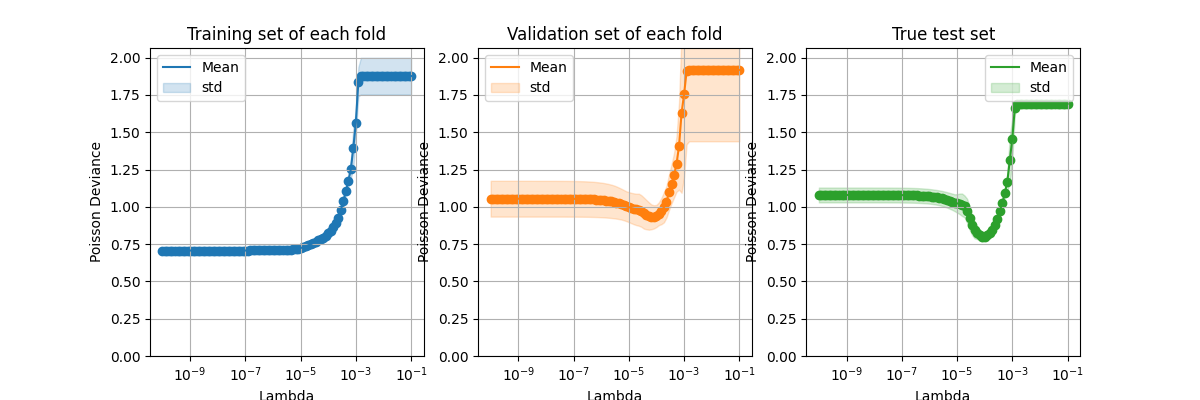
\includegraphics[width=0.75\linewidth]{extra_plots/poisson_regression_lasso_deviance_vs_lambda_no_log_transform.png}
    }
    % \hfill
    \\
    \subfloat[Log-Transformed and Normalized Data.]{
        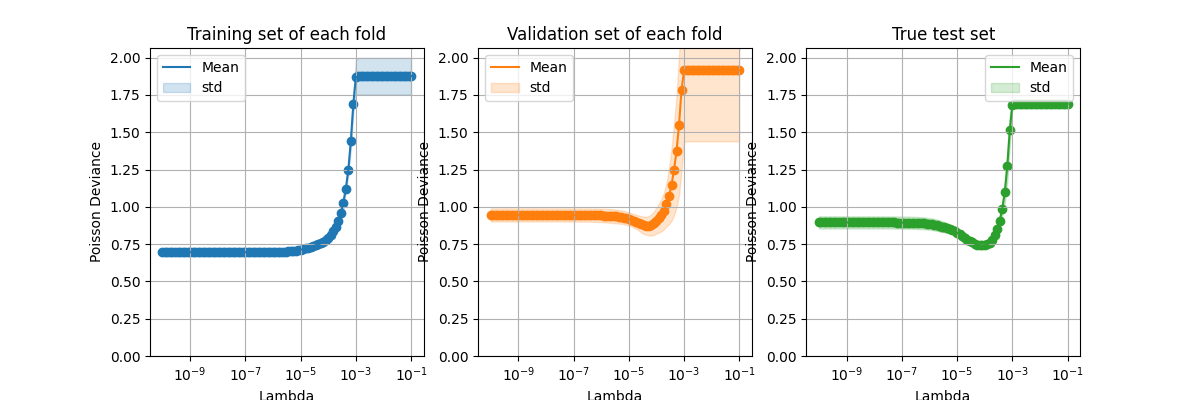
\includegraphics[width=0.75\linewidth]{extra_plots/poisson_regression_lasso_deviance_vs_lambda_log_transform.png}
    }
    \caption{The mean and standard deviation of the mean Poisson deviation score for the subset of the training set of each fold (left, blue), the hold out set for of the train set for each fold (middle, orange), and the full test set (right, green).}
    \label{fig:deviance_vs_lambda_poisson}
\end{figure}

From Figure~\ref{fig:deviance_vs_lambda_poisson}, we clearly see that lowest value for the mean Poisson deviance is convex at $\lambda \approx 10^{-4}$. In fact, we find that the best value for $\lambda$ is $1\cdot 10^{-4}$ for the just normalized data, and $8\cdot 10^{5}$ for the log-transformed data.
Using these values, we obtain the following values:
\begin{table}[htbp]
    \centering
    \begin{tabular}{l|cc}
         \toprule
         & Train & Test \\
         \midrule
         Normalized & $0.82125$ & $0.79864$ \\
         Log-Transformed \& Normalized & $\mathbf{0.77761}$ & $\mathbf{0.74252}$ \\
         \bottomrule
    \end{tabular}
    \caption{The mean Poisson deviation values for the best \textbf{Poisson regression model} obtained using \textbf{$L_1$-lasso} for the different datasets. We highlight in bold the best value of the table for each of the data splits.}
    \label{tab:deviation_poisson_l1}
\end{table}

As we can use $L_1$-regularization for feature selection, we plot the coefficients for the individual parameters over the values of $\lambda$. As we have 32 parameters in total, we add the plots in the Appendix (see Figure~\ref{fig:coefficients_lambda_normalized} and Figure~\ref{fig:coefficients_lambda_log_transformed_and_normalized}), as, while they are interesting, these plots are not at the core of this question. 

We remark that, especially in the case where we use the log-transformed data (see Figure~\ref{fig:coefficients_lambda_log_transformed_and_normalized}), all the features found by the stepwise search with the BIC score are have non-zero coefficients in the lasso regression. On the other hands, many values found by the AIC stepwise search have coefficients of zero.

However, lasso-regression, if interpreted as a feature selector, finds a different set of features as stepwise seach with BIC. For example, \texttt{numberOfVersionsUntil:} has non-zero coefficients at at the optimal value for $\lambda$, which is not included in the set of features found by any search algorithm for stepwise model search.

\subsection{Discussion}

\textbf{AIC vs BIC.}
It is clear that BIC outperforms AIC. Not only does BIC stops as soon as the test deviance increases by just looking at the training set, which is not the case for AIC.

Furthermore, while AIC keeps adding features to the model, we remark that every feature from the BIC model is included in the set of features found when using AIC (see Table~\ref{tab:coefficients_poisson_stepwise_normalized} and Table~\ref{tab:coefficients_poisson_stepwise_log_normalized}).

Therefore, together with the results from Table~\ref{tab:accuracy_logistic_stepwise}, which state that AIC overfits to the training set, whereas BIC is more robust to overfitting, we can conclude that, empirically, BIC is better at scoring models than AIC.

\textbf{Coefficients of the Model.}
Interesting, when looking at the coefficients of the learned model, we see that a very delicate balance is being optimized. For example, when looking at the coefficient for the \texttt{cbo} variable, we see that increasing it has a negative impact on the prediction, even though it has a positive coefficient (see Table~\ref{tab:coef_stepwise_logistic_normalized}).
% Comparing the coefficient of this variable to the coefficient of 
On the other hand, the oracle model for the binary classification of whether a bug is included in the code has a value around 6 times higher than in the Poisson regression model found by stepwise model selection (see Table~\ref{tab:features_coeff_logistic_normalized} in the Appendix).

This does not mean that \texttt{cbo} cannot give information on the number of bugs included in the code, but as the other variables, such as \texttt{numberOfMethodsInherited} or \texttt{weightedAgeWithRespectTo:} might better modeling capabilities of the number of bugs, removing the information of \texttt{cbo} can the Poisson regression model to better model the number of bugs.

\textbf{P-values.}
We report on the p-values of the coefficients.
While we found that AIC performs worse than BIC, we further notice that, every feature added additionally by AIC has a high p-value. 

For example, in Table~\ref{tab:coef_stepwise_logistic_normalized}, we have a p-value of 0.052 for the \texttt{noc} variable, which makes the test deviance increase. Therefore, not adding it is better.

Furthermore, using a threshold value of 0.05 or 0.01, we would reject that \texttt{noc} has an influence on the prediction of the number of bugs.

\textbf{Comparison of $L_1$-regularization and Stepwise Model Selection.}
We see that the model found by stepwise model selection with BIC as scoring outperforms the best model found by $L_1$-regularization (compare Table~\ref{tab:mean_poisson_deviation_poisson_regression_step_search} and Table~\ref{tab:deviation_poisson_l1}).

Furthermore, we see that $L_1$-regularization not only selects way more features in the model with the best value for $\lambda$, estimated on the hold out set, but out of the selected features, all of them overlap with the features found by stepwise search (see the coefficients in Figure~\ref{fig:coefficients_lambda_normalized} and Figure~\ref{fig:coefficients_lambda_log_transformed_and_normalized}).

\section{Logistic Regression}

We constructed a binary target variable \texttt{bugbin}, where $\texttt{bugbin}=1$ if $\texttt{bugs}\ge1$ and 0 otherwise. 
% A logistic regression model was fitted and forward stepwise selection using AIC was performed on the training set.
We perform the same analysis as done in the previous section, however, instead of reporting on the mean Poisson deviation, we report on the mean accuracy. 

% Due to the change in the parametrization of the model, we have to adjust our definition for $\delta_i$.

% We know from the lecture that 
% \begin{equation}
%     \frac{\mathbb{E}[y\mid x + \delta]}{\mathbb{E}[y\mid x]} \propto \exp(\beta_i \cdot \delta_i)\;.
% \end{equation}
% Therefore


\subsection{Stepwise Model Selection}

We observe the same relationship between the AIC and BIC search as in Section~\ref{sec:poisson_stepwise}.
Therefore, we will only report on the stepwise search using BIC and omit to report on the performance of the AIC search.
We plot in Table~\ref{fig:accuracy_logistic_regression} the evolution of the accuracy of the different models using stepwise search. 
We omit a detailed discussion of the plots, as we would use the same arguments denoted in Section~\ref{sec:poisson_stepwise}.

\begin{figure}[t]
    \centering
    % {\textbf{Log-Transformed \& Normalized} Data} \\
    \subfloat[Using \textbf{Normalized} Data.]{
        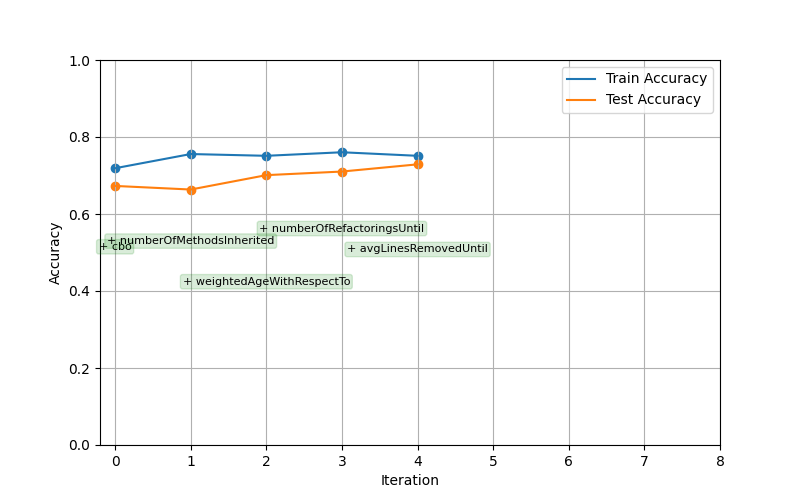
\includegraphics[width=0.45\linewidth]{extra_plots/logistic_regression_stepwise_accuracy_history_bic_no_log_transform.png}
    }
    \hfill
    \subfloat[Using \textbf{Log-Transformed \& Normalized}.]{
        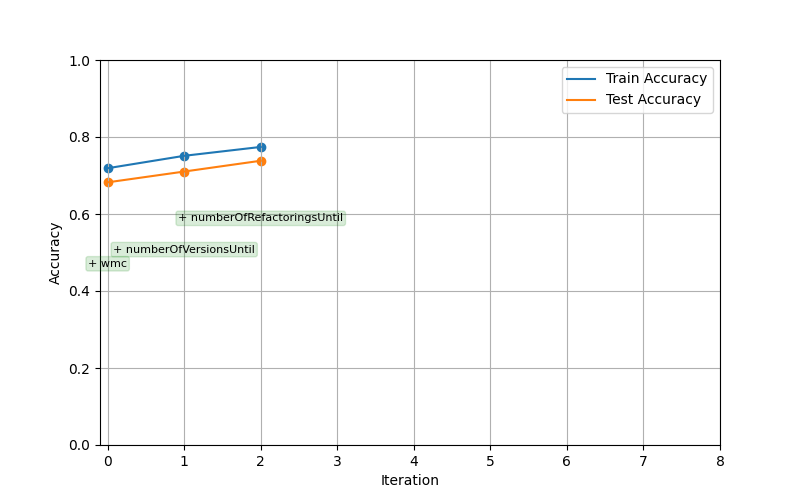
\includegraphics[width=0.45\linewidth]{extra_plots/logistic_regression_stepwise_accuracy_history_bic_log_transform.png}
    }
    \caption{Train and test deviance of the \textbf{Logistic regression} when using \textbf{stepwise model selection} with \textbf{BIC}. Note that the green boxes starts with + denote which feature has been added to the model.}
    \label{fig:accuracy_logistic_regression}
\end{figure}
We therefore obtain the following accuracies for the stepwise search:
% 0.751152, Test accuracy: 0.728972
% 0.774194, Test accuracy: 0.738318
\begin{table}[htbp]
    \centering
    \begin{tabular}{l|cc}
         \toprule
         \textbf{Set} & \textbf{Train} ($\uparrow$) & \textbf{Test} ($\uparrow$) \\
         \midrule
         Normalized & $0.751152$ & $0.728972$ \\
         Log-Transformed \& Normalized & $\mathbf{0.774194}$ & $\mathbf{0.738318}$ \\
         \bottomrule
    \end{tabular}
    \caption{The mean accuracy for the best \textbf{Logistic} regression model obtained using \textbf{stepwise model search} for the different datasets. We highlight in bold the best value of the table for each of the data splits.}
    \label{tab:accuracy_logistic_stepwise}
\end{table}

Similarly, we report on the values of the coefficients and their influence on the prediction in Table~\ref{tab:coef_stepwise_logistic_normalized} for the normalized dataset and in Table~\ref{tab:coef_stepwise_logistic_log_transform} for the log-transformed and normalized features.

% \todo[inline]{Talk about the $F_1$ metric, and false positive/false negatives.}

\begin{table}[htbp]
    \centering
    \begin{tabular}{l c c c c}
        \toprule
        \textbf{Variable} & \textbf{Coefficient} & $\frac{\mathbb{E}[y\mid x+\delta_i]}{\mathbb{E}[y\mid x]}$ & \textbf{p-value} & \textbf{95\% CI} \\
        \midrule
        Intercept & $-0.406$ & -- & $0.024$ & $[-0.759,\,-0.054]$ \\
        \texttt{cbo} & $1.289$ & $0.963$ & $<0.001$ & $[0.777,\,1.801]$ \\
        \texttt{numberOfMethodsInherited} & $0.694$ & $1.095$ & $0.012$ & $[0.153,\,1.235]$ \\
        \texttt{weightedAgeWithRespectTo:} & $0.549$ & $1.021$ & $0.004$ & $[0.178,\,0.921]$ \\
        \texttt{numberOfRefactoringsUntil:} & $-0.558$ & $3.951$ & $0.008$ & $[-0.969,\,-0.147]$ \\
        \texttt{avgLinesRemovedUntil:} & $0.728$ & $0.959$ & $0.019$ & $[0.119,\,1.337]$ \\
        \bottomrule
    \end{tabular}
    \caption{The coefficients of the Logistic regression model found using \textbf{stepwise search} with \textbf{BIC} for the \textbf{normalized} data.}
    \label{tab:coef_stepwise_logistic_normalized}
\end{table}

\begin{table}[htbp]
    \centering
    \begin{tabular}{l c c c c}
        \toprule
        \textbf{Variable} & \textbf{Coefficient} & $\frac{\mathbb{E}[y\mid x+\delta_i]}{\mathbb{E}[y\mid x]}$ & \textbf{p-value} & \textbf{95\% CI} \\
        \midrule
        Intercept & $-0.621$ & -- & $0.001$ & $[-0.974,\,-0.268]$ \\
        \texttt{wmc} & $0.986$ & -- & $<0.001$ & $[0.506,\,1.466]$ \\
        \texttt{numberOfVersionsUntil:} & $1.014$ & -- & $<0.001$ & $[0.512,\,1.517]$ \\
        \texttt{numberOfRefactoringsUntil:} & $-0.482$ & -- & $0.011$ & $[-0.853,\,-0.112]$ \\
        \bottomrule
    \end{tabular}
    \caption{The coefficients of the Logistic regression model found using \textbf{stepwise search} with \textbf{BIC} for the \textbf{log-transformed \& normalized} data.}
    \label{tab:coef_stepwise_logistic_log_transform}
\end{table}

\subsection{$L_1$-Lasso Regularization}

We run the same code as in Section~\ref{sec:l1_lasso_poisson}, namely logistic regression with 5-fold cross validation on the training set.

As shown in Figure~\ref{fig:deviance_vs_lambda_poisson}, using both datasets results in almost equal plots of the the accuracy (deviation in the Figure) when plotted against the value of $\lambda$. Therefore, we move the accuracy-vs-lambda-plot for the normalized data to the Appendix (Figure~\ref{fig:logistic_regression_lasso_deviance_vs_lambda_no_log_transform}), and report on the log-transformed and normalized data in Figure~\ref{fig:logistic_regression_lasso_deviance_vs_lambda_log_transform}. 

\begin{figure}[tp]
    \centering
    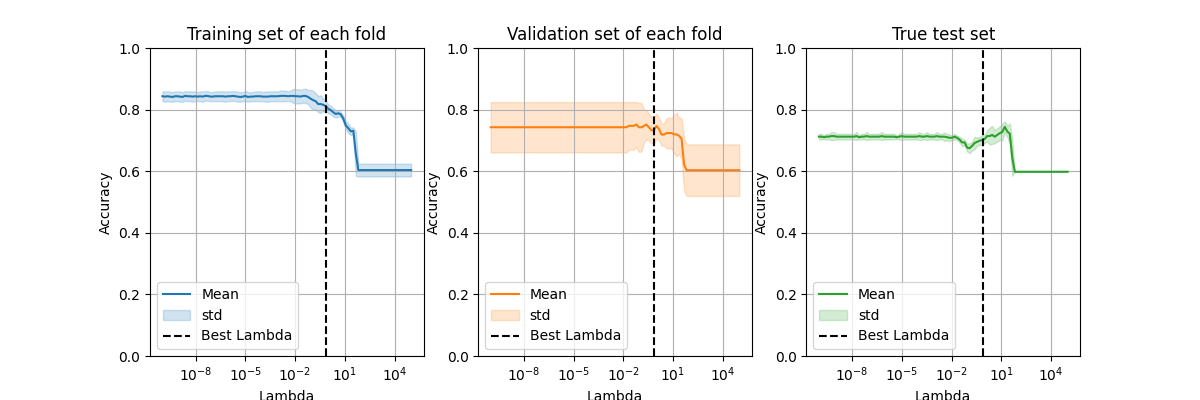
\includegraphics[width=\linewidth]{extra_plots/logistic_regression_lasso_deviance_vs_lambda_log_transform.png}
    \caption{Accuracy w.r.t. $\lambda$ for the $L_1$-lasso \textbf{logistic} regression for the log-transformed and normalized data.}
    \label{fig:logistic_regression_lasso_deviance_vs_lambda_log_transform}
\end{figure}

Surprisingly, we observe that the estimated test accuracy from the fold does not (highly) correlate with the true test set accuracy. Therefore, the value we find for best lambda, based on the estimated validation accuracy, is not at a maximum of the true test accuracy.

We again report on the optimized coefficients w.r.t. $\lambda$ in Figure~\ref{fig:logistic_regression_lasso_coefficients_log_transform} in the Appendix. We also add a table containing the coefficients of the logistic regression model learned with the best $\lambda$ value for the normalized dataset in the Appendix (Table~\ref{tab:features_coeff_logistic_normalized}).

Using the best value for $\lambda$ that we found using the hold out set of each fold, we obtain the following accuracies:
\begin{table}[htbp]
    \centering
    \begin{tabular}{l|cc}
         \toprule
         \textbf{Set} & \textbf{Train} ($\uparrow$) & \textbf{Test} ($\uparrow$) \\
         \midrule
          Normalized & $\mathbf{0.81105}$ & $\mathbf{0.74766}$ \\
         Log-Transformed \& Normalized & $0.81567$ & $0.719626$ \\
         \bottomrule
    \end{tabular}
    \caption{The mean accuracy for the best \textbf{Logistic} regression model obtained using \textbf{$L_1$-regularization} for the different datasets. We highlight in bold the best value of the table for each of the data splits.}
    \label{tab:accuracy_logistic_regression_lasso}
\end{table}

\subsection{Discussion}

First, let us discuss the results from the $L_1$-lasso regression.

\textbf{Discrepancy in Table~\ref{tab:accuracy_logistic_regression_lasso}.}
One of the most surprising results is contained in Table~\ref{tab:accuracy_logistic_regression_lasso}, where the log-transformed data got outperformed by the just normalized data. This goes goes against the trend we observed all along the report, namely that the log-transformation of the data achieves better results than the normalized results.

However, we can explain the results from Table~\ref{tab:accuracy_logistic_regression_lasso}. To this end, let us first look at the accuracy vs lambda plot of the logistic regression using the log-transformed data (Figure~\ref{fig:accuracy_logistic_regression}).
In this Figure, we can clearly see that best accuracy on the test set is obtained with $\lambda \approx 16.0$, where the mean accuracy jumps to approximately $0.7439$.
However, the highest value on the estimated accuracy on the hold out set (middle plot of the Figure) is far from the optimal $\lambda$ for achieving maximal test accuracy. 

% On the other hand, when we look at the same plots but for the just normalized data (see Figure~\ref{fig:logistic_regression_lasso_deviance_vs_lambda_no_log_transform}), we see that 
% the best lambda that was found using the hold out set matches with one of the maxima of the accuracy vs lambda curve (green curve in that Figure). 

% \todo[inline]{Add this observation to a new argument.}
% It is noteworthy to highlight that the curve on the test set (green plot) is almost maximized for any $\lambda < 10^1$. 

Therefore, while the logistic regression on the log-transformed and normalized dataset has a potential for a higher accuracy, the logistic regression on the normalized data reaches a better peak. 

\textbf{Found Features with $L_1$-Regularization.}
Let us now look at the coefficients for the best logistic regression model found when adding $L_1$-regularization on the normalized data (Table~\ref{tab:features_coeff_logistic_normalized}).

Note that interpreting the value, or even the sign, of the coefficients of a logistic regression fitted on log-transformed data is not feasible, as the impact of the value change w.r.t. the value of the input.

To gain insights from this analysis, we abstain from investigating the coefficients of the model found at $\lambda=$Best Lambda from Figure~\ref{fig:logistic_regression_lasso_deviance_vs_lambda_no_log_transform}, as we see from Figure~\ref{fig:coefficients_lambda_normalized} and Figure~\ref{fig:coefficients_lambda_log_transformed_and_normalized} that for extremely low $\lambda$ values, the variance is very high.

Furthermore, if $\lambda\approx 0$, we may risk overfitting on the training data, and therefore obtain a meaningless model.
Therefore, we cheat and use $\lambda = 1$, which maximizes the test accuracy for this case.

% We obtain the optimal test accuracy with $\lambda = 1$, and therefore  

When looking at the three most important features, we have that a coefficient for \texttt{cbo}, which denotes the Coupling Between Objects, and has a positive coefficient. This makes sense, as increasing the number of objects coupled together, if one of these objects has a bug, then all of them have a bug.
Similarly, \texttt{noc}, which stands for Number Of Children, has a strong influence on the prediction of a bug. This follows from the last argument.

Surprisingly, in this model, the number of methods (\texttt{numberOfMethods}) has a negative impact on the prediction. 

We remark that many many features that we expect to correlate with the prediction have a strong (positive or negative) influence on the prediction. For example, \texttt{numberOfRefactoringsUntil:} reduces the odds of predicting a bug by 75\% for every time a refactoring has been done. This is biased data, as code is being refactored if it contains bugs, or is prone to contain bugs.

We remark that we are unable to relate all features with respect to each other, as while the features are normalized, their value might not change the same way. For example, changing the number of lines of code will result in a much smaller difference in input (which we denote as $\Delta x$) compared to \texttt{numberOfRefactoringsUntil:} for example.

A joint analysis is way beyond the scope of this assignment, as we would need to look at the distribution of the features and the coefficients jointly, which, for 32 feature, is very vast.

\textbf{Comparison between $L_1$-Regularization and Stepwise Model Selection.}
Let us now compare the results of the $L_1$-regularization and the results from the stepwise model selection for the logistic regression.

Comparing the best found accuracies, we see that, while the log-transformed dataset outperforms the just normalized dataset when using stepwise model selection (see Table~\ref{tab:accuracy_logistic_stepwise}), the trend is reversed\footnote{See previous argument.} in the $L_1$-regularization case (see Table~\ref{tab:accuracy_logistic_regression_lasso}).

Furthermore, we see that $L_1$-regularization allows to find better performing models than stepwise model selection. 
We will discuss this in more detail in Section~\ref{sec:discussion:differences}.

The most obvious difference between both search methods is the number of features found. Whereas stepwise feature selection finds very few features (when using BIC as scoring), $L_1$ regression sets coefficients to zero only for high values of $\lambda$, where the model then degrades do to the added constraints by the regularization.

When looking at the coefficients, interestingly, the fitted models found by the stepwise model selection have drastically different coefficients for some of the parameters. For example, on the normalized data, stepwise selection finds a coefficient of $1.289$ for the \texttt{cbo} variable (see Table~\ref{tab:coef_stepwise_logistic_normalized}), in the \textit{oracle} model, we have a coefficient of $3.020$, which drastically changes the influence of the feature on the prediction. 

Investigating whether setpwise model selection could benefit from having one of the coefficient fixed from the oracle model would be an interesting future work.

\textbf{Accuracy Metric.}
While the accuracy metric is a good metric to observe how good a classification model performs, we wish to comment on the metric used.

Other popular metrics used in classification are the $F_1$ score, the selectivity, and specificity.
Which one is optimal depends on the application of the model.

We believed that, for this task, the accuracy gives us enough information to compare the different model.
However, if someone wants to, for example, develop a software that raises a warning if the probability for a bug in the function is high, then false positives are really undesired in the general case. Note that some cases have the type of error priority flipped; For example, when programming for NASA, raising a false positive is less impactful than having a false negative, and shipping code that contains a bug.

\section{Discussion --- Differences Between $L_1$-regularization and Stepwise Model Selection}

% \subsection{Differences between Stepwise Model Selection and $L_1$-Regularization}
\label{sec:discussion:differences}

Let us now comment on the differences between the two search algorithms.
A questions one might --- rightfully --- ask is \textit{which search algorithm is better?}
We believe that this question has no simple answer.

In this report alone, we have seen two cases of when one search performs better than the other; In our case, when modeling the number of bugs in the functions, we find that stepwise model selection outperforms $L_1$-regularization, whereas for predicting the existence of at least one bug, we see have found that $L_1$-regularization outperforms stepwise model selection, with even more stable accuracies.

We hypothesis that, in the case of the modeling of the number of bugs, simpler models outperform complex ones. We argue that this is due to the simpler model capturing the general trend, instead of potential noise that might correlate with the response variable in the train set but not in the test set.

If a model is dependent on a lot of variables, the probability that one of the variables changes by chance (e.g., because of noise, or hidden confounders), is very high, and therefore, the prediction might be off because of this arbitrary change.
Note that this is different from the overfitting phenomenon, which also contributes to a model having a higher number of features. However, a model having a lot of features does not necessarily overfit, whereas the probability that a model has a lot of features, given that it has overfit, is much higher.

On the other hand, for the binary prediction case, we can make use of more features, as the magnitude of the prediction is not very relevant, but rather if the prediction crosses the 0.5 boundary.
Therefore, if some noise is being added the the features, a complex model could still have the same prediction in the logistic regression case, whereas the difference to the original prediction could be quite large for the Poisson regression.

% \subsection{Finding One Bug vs Finding the Number of Bugs}

\pagebreak

% The table below shows the estimated coefficients of the selected Poisson regression model, together with standard errors, z-statistics, p-values, and 95\% confidence intervals.

% \begin{table}[h]
% \centering
% \begin{tabular}{lccccc}
% \hline
% Variable & Coefficient & Std. Error & z & p-value & 95\% CI \\
% \hline
% Intercept & -1.9665 & 0.189 & -10.388 & $<0.001$ & [-2.337, -1.595] \\
% cbo & 0.0454 & 0.004 & 12.728 & $<0.001$ & [0.038, 0.052] \\
% numberOfMethodsInherited & 0.0167 & 0.003 & 5.249 & $<0.001$ & [0.010, 0.023] \\
% weightedAgeWithRespectTo & 0.0117 & 0.002 & 5.241 & $<0.001$ & [0.007, 0.016] \\
% avgLinesAddedUntil & 0.0084 & 0.003 & 3.097 & 0.002 & [0.003, 0.014] \\
% noc & 0.1789 & 0.092 & 1.945 & 0.052 & [-0.001, 0.359] \\
% \hline
% \end{tabular}
% \end{table}

% All selected predictors have positive coefficients, indicating that higher structural complexity or more extensive code evolution is associated with a higher expected number of bugs. Most variables are statistically significant at the 5\% level, while \texttt{noc} shows a borderline effect.

% The predictive performance of the selected model was evaluated on the test set using Poisson deviance:
% \begin{itemize}
% \item \textbf{Deviance:} 0.81
% \end{itemize}

% \subsubsection{LASSO regularization}

% To model the number of bugs, we applied Poisson regression with L1 (LASSO) regularization. All predictors were standardized prior to model fitting, which is necessary for LASSO to penalize coefficients in a comparable way. The regularization parameter $\lambda$ was selected on the training set using 5-fold cross-validation, with \textbf{Poisson deviance} as the evaluation criterion.

% Cross-validation selected the following value:
% \begin{itemize}
% \item \textbf{Selected $\lambda$:} 0.166
% \end{itemize}

% Under the selected regularization strength, the LASSO Poisson model retained only a single non-zero coefficient:
% \begin{itemize}
% \item \textbf{Selected feature:} \texttt{cbo}
% \end{itemize}

% The final LASSO-selected model was evaluated on the test set:
% \begin{itemize}
% \item \textbf{Deviance:} 1.279
% \end{itemize}

% This deviance value is higher than that obtained by the stepwise Poisson model, indicating a trade-off between model simplicity and predictive accuracy.

% \subsubsection{Comparison of stepwise and LASSO}
% \begin{figure}[t]
%     \centering
%     \subfloat[Logistic regression (stepwise)]{
%         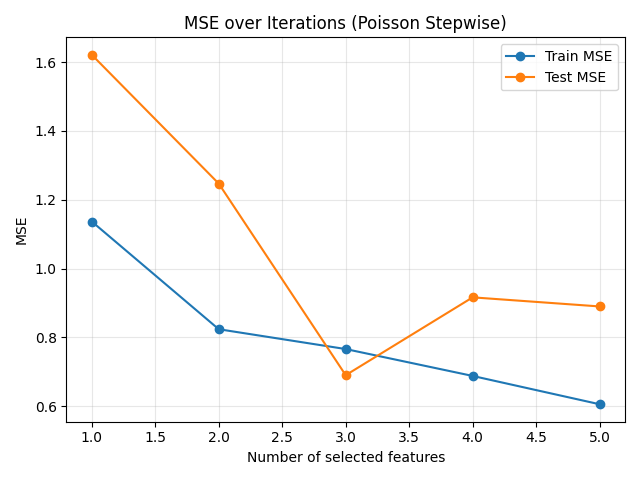
\includegraphics[width=2.5in]{MSE_PS.png}
%     }
%     \hfill
%     \subfloat[Poisson regression (stepwise)]{
%         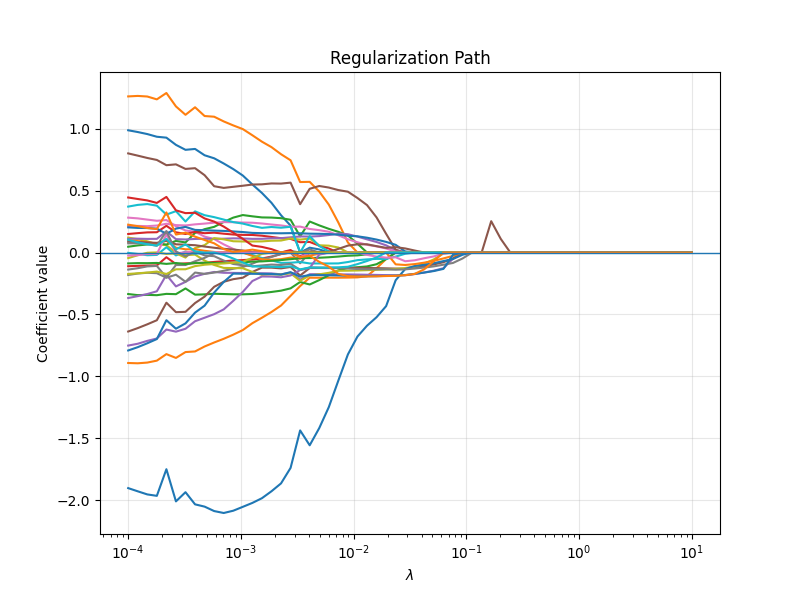
\includegraphics[width=2.5in]{reg_PL.png}
%     }
%     \caption{MSE over iterations.}
%     \label{stepwise vs LASSO}
% \end{figure}
% The stepwise-selected model includes five predictors and achieves a lower test Poisson deviance (0.81), indicating better predictive performance. In contrast, Poisson LASSO yields a much sparser model with only one predictor but results in a higher deviance (1.279). For this dataset, stepwise selection appears more suitable when predictive accuracy is the primary goal.

% As seen from Figure 3, the stepwise selection shows that Poisson regression is highly sensitive to overfitting and that adding more predictors beyond the lowest point degrades performance greatly.

%  In the LASSO regularization case, as the parameter $\lambda$ increases, most coefficients are rapidly shrunk to zero, and only few predictors remain active for moderate value of $\lambda$. Consequently, cross-validation select a strong regularization level, producing an extremely sparse model that retains only the most dominant feature.

% Comparing these two approaches, stepwise selection achieves a better balance between model complexity and predictive performance by retaining a small but informative set of predictors. On the other hand, LASSO enforces excessive sparsity, which leads to underfitting and slightly worse performance. For this dataset, stepwise selection is more suitable for Poisson regression.

% \subsection{Logistic regression}

% \subsubsection{Stepwise model selection}

% We constructed a binary target variable \texttt{bugbin}, where $\texttt{bugbin}=1$ if $\texttt{bugs}\ge1$ and 0 otherwise. A logistic regression model was fitted and forward stepwise selection using AIC was performed on the training set.

% The final model includes the following predictors:
% \begin{itemize}
% \item \texttt{cbo}, \texttt{numberOfMethodsInherited}, \texttt{weightedAgeWithRespectTo},
% \texttt{numberOfRefactoringsUntil}, \texttt{avgLinesRemovedUntil}, \texttt{noc}, \texttt{dit}
% \end{itemize}

% \begin{table}[h]
% \centering
% \begin{tabular}{lccccc}
% \hline
% Variable & Coef. & Std. Err. & z & p-value & 95\% CI \\
% \hline
% Intercept & -3.8173 & 0.629 & -6.069 & $<0.001$ & [-5.050, -2.585] \\
% cbo & 0.1191 & 0.025 & 4.845 & $<0.001$ & [0.071, 0.167] \\
% numberOfMethodsInherited & 0.0296 & 0.021 & 1.440 & 0.150 & [-0.011, 0.070] \\
% weightedAgeWithRespectTo & 0.0168 & 0.006 & 2.894 & 0.004 & [0.005, 0.028] \\
% numberOfRefactoringsUntil & -1.3044 & 0.525 & -2.486 & 0.013 & [-2.333, -0.276] \\
% avgLinesRemovedUntil & 0.0643 & 0.024 & 2.675 & 0.007 & [0.017, 0.111] \\
% noc & 0.7458 & 0.345 & 2.161 & 0.031 & [0.069, 1.422] \\
% dit & 0.8081 & 0.416 & 1.944 & 0.052 & [-0.007, 1.623] \\
% \hline
% \end{tabular}
% \end{table}

% The final model was evaluated on the test set:
% \begin{itemize}
% \item \textbf{Accuracy:} 0.720
% \end{itemize}

% \subsubsection{LASSO regularization}

% In the \texttt{sklearn} implementation, the regularization strength is controlled by parameter $C$ (with $\lambda = 1/C$). Cross-validation selected a large $C$, resulting in weak regularization and a model retaining many predictors.

% The test-set performance was:
% \begin{itemize}
% \item \textbf{Accuracy:} 0.729
% \end{itemize}

% \subsubsection{Comparison of stepwise and LASSO}
% \begin{figure}[t]
%     \centering
%     \subfloat[Logistic regression (LASSO)]{
%         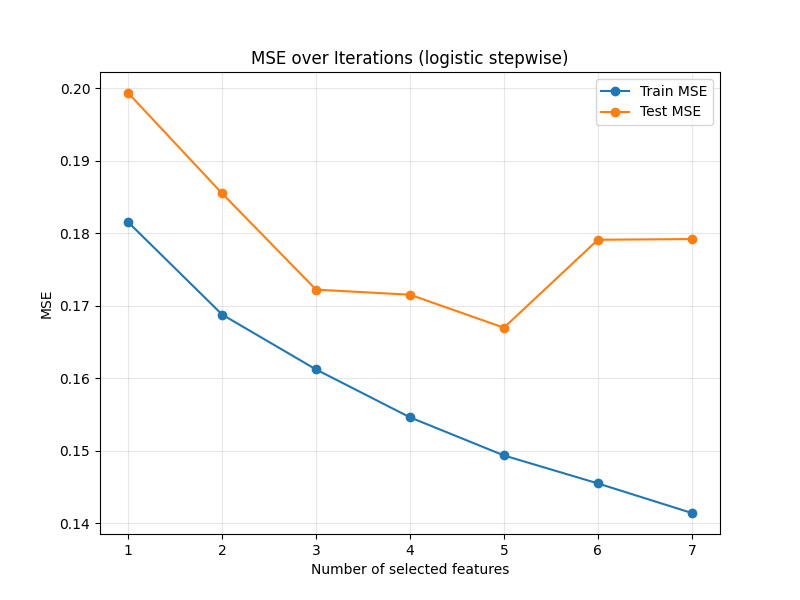
\includegraphics[width=2.5in]{MSE_LS.png}
%     }
%     \hfill
%     \subfloat[Logistic regression (stepwise)]{
%         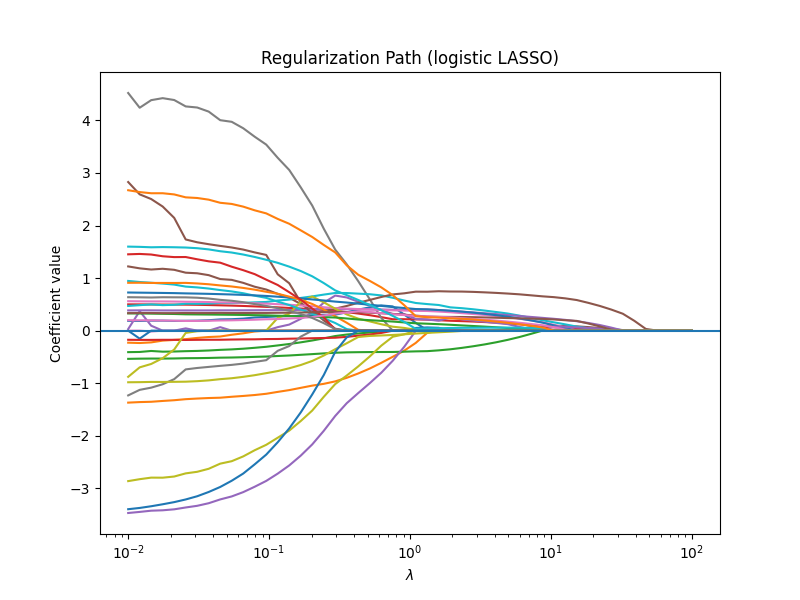
\includegraphics[width=2.5in]{reg_LL.png}
%     }
%     \caption{MSE and Regularization path.}
%     \label{fig:logistic_comparison}
% \end{figure}

% As seen from figure 4, the stepwise selection curve shows that the training MSE decreases monotonically as more features are added, while the test MSE reaches a minimum at an intermediate model size, after which increases slightly, showing stepwise selection explicitly controls overfitting by stopping the inclusion of more predictors once performance gets worse.

% On the other hand, the logistic LASSO regularization path shows a gradual decreasing of coefficients as the penalty parameter $\lambda$ increases. Rather than eliminating predictors abruptly, many coefficient remain non-zero over a wide range of $\lambda$. As a result, cross-validation selects a relatively weak regularization strength, leading to a model that retains multiple correlated predictors.

% Overall, these results indicate a key difference between these two approaches. Stepwise selection yields a more compact and easily interpretable model by directly limiting the amount of features, while LASSO controls complexity through coefficient shrinkage and achieves slightly better predictive performance by retaining a larger set of features.

% \pagebreak


\appendix
\chapter{Appendix}

\section{Statement on the Useage of Gen. AI}
\begin{itemize}
    \item \textbf{Felix Céard-Falkenberg}\newline
Unless stated otherwise, all code, text, and math derivations have been entirely thought and written by me with no external help --- both for gen. AI and wolframalpha anc co.

We used Claude 4.5 Opus for generating the plots for Figure~\ref{fig:mse_naive_better} as the plot is not a core of the assignment, and only aids in understanding our own results. Note that we (heavily) modified the code generated by Claude.

For question 2 of the assignment, we used ChatGPT 5.2 to help us with some of the math of the derivations. The end product is ~90\% my own, indepent work. 
Most of the A.I. being used for question 2 got scrapped as it did not add any value to the report. The most notable scrapped work was finding some result to $\mathbb{E}\left[ \frac{f_1^2}{2f_2} \right]$, but as both are dependent, only very limited results were found by ChatGPT.\!\footnote{This may also be due to my bad prompting.}

% I used ChatGPT to help find literature on the properties of integration, differentiation.

% Furthermore, when researching for denoising algorithms, I used ChatGPT to get a general overview of the available general denoising algorithms. After finding the Bayesian denoising algorithm, I used Claude 4.5 Sonnet to write the code for the Bayesian denoising algorithm (based on existing code for Bayesian denoising implemented for 2D images). As the exact algorithm is not at the core of the assignment or the course, and that the results of both denoising methods are very similar, I believe that this usage is acceptable.


We used Claude 4.5 Opus for generating the plots for Figure~\ref{fig:mse_naive_better} as the plot is not a core of the assignment, and only aids in understanding our own results. Note that we (heavily) modified the code generated by Claude. 

    For Part B, we used ChatGPT to insert some value from lists into latex tables, but we made sure that all values lined up.


    \item \textbf{Yiquan Hu}\newline
    For Part B, we used ChatGPT to generate required code for stepwise selection with the permissions stated in the assignment instructions and also consulted ChatGPT for general suggestions on parameter adjustment. All analysis, results and interpretations were produced by us. We only used ChatGPT lightly refine the academic word of some sentences without adding new content.
    
\end{itemize}

\section{Additional Tables}

\begin{table}[h]
    \centering 
    \caption*{$p_i \sim 0.02 \cdot \mathrm{Beta}(1, 3)$}
    \begin{tabular}{c c|c c c}
        \toprule
        & & \multicolumn{1}{|c|}{${N}=500$} & \multicolumn{1}{c|}{${N}=1000$} & \multicolumn{1}{c}{${N}=5000$} \\
        \midrule
        \multicolumn{2}{c|}{${\hat{\mathbf{N}}}$} & $572.21 \variance{249}$ & $1102.16 \variance{327}$ & $5165.82 \variance{579}$  \\
        \multicolumn{2}{c|}{\textbf{Error} (\%)} & $14.44$ & $10.22$ & $3.32$ \\
        % \hline
        \multicolumn{2}{c|}{${\hat{\mathbf{\sigma}}}_{\hat{N}}$} & $223.18 \variance{168}$ & $288.20 \variance{146}$ & $568.22 \variance{96}$\\
        % \hline
        \multirow{2}{*}{\textbf{C.I.}} & $\alpha = 0.05$ & $[296.06 \variance{80}; 1241.40 \variance{822}]$ & $[688.71 \variance{147}; 1861.17 \variance{749}]$ & $[4189.85 \variance{421}; 6432.61 \variance{798}]$
        \\
        % 
        & $\alpha = 0.01$ & $[248.36 \variance{58}; 1610.48 \variance{1203}]$ & $[602.47 \variance{115}; 2212.82 \variance{975}]$ & $[3932.12 \variance{381}; 6903.90 \variance{882}]$ \\
        \midrule
        \multirow{2}{*}{\textbf{Coverage} (\%)} & $\alpha = 0.05$ & $94.60 \variance{22}$ & $94.00 \variance{23}$ & $94.60 \variance{22}$ \\
        & $\alpha = 0.01$ & $98.90 \variance{10}$ & $98.80 \variance{10}$ & $98.90 \variance{10}$ \\
        \multicolumn{2}{c|}{\textbf{Bias} ($\approx$)} & $5\ 214$ & $10\ 436$ & $27\ 495$ \\
        \multicolumn{2}{c|}{\textbf{Variance} ($\approx$)} & $78\ 120$ & $104\ 540$ & $332\ 210$ \\
        \multicolumn{2}{c|}{\textbf{MSE} ($\approx$)} & $83\ 334$ & $114\ 977$ & $359\ 705$ \\
        \bottomrule
    \end{tabular}
    \caption{Result from $1000$ MC simulations for estimating $\hat{N}$. For each value, we report on the mean (black) and standard deviation (gray). We omit the digits after the decimal point for the standard deviation for brevity.
    The Error (\%) is the absolute difference between the estimated and the true value of $N$, divided by the true value of $N$.}
    \label{tab:problem_2_results_beta_1_3}
\end{table}

\begin{table}[h]
    \centering 
    \caption*{$p_i \sim 0.01 \cdot \mathrm{Beta}(2, 2)$}
    \begin{tabular}{c c|c c c}
        \toprule
        & & \multicolumn{1}{|c|}{${N}=500$} & \multicolumn{1}{c|}{${N}=1000$} & \multicolumn{1}{c}{${N}=5000$} \\
        \midrule
        \multicolumn{2}{c|}{${\hat{\mathbf{N}}}$} & $582.90 \variance{314}$ & $1093.58 \variance{294}$ & $5128.88 \variance{565}$  \\
        \multicolumn{2}{c|}{\textbf{Error} (\%)} & $16.58$ & $9.36$ & $2.58$ \\
        % \hline
        \multicolumn{2}{c|}{${\hat{\mathbf{\sigma}}}_{\hat{N}}$} & $235.15 \variance{275}$ & $281.72 \variance{121}$ & $561.35 \variance{93}$\\
        % \hline
        \multirow{2}{*}{\textbf{C.I.}} & $\alpha = 0.05$ & $[297.63 \variance{84}; 1303.01 \variance{1391}]$ & $[687.38 \variance{139}; 1831.89 \variance{634}]$ & $[4164.29 \variance{411}; 6379.84 \variance{776}]$
        \\
        % 
        & $\alpha = 0.01$ & $[249.11 \variance{59}; 1716.36 \variance{2272}]$ & $[602.16 \variance{110}; 2171.47 \variance{808}]$ & $[3909.42 \variance{373}; 6844.99 \variance{858}]$ \\
        \midrule
        \multirow{2}{*}{\textbf{Coverage} (\%)} & $\alpha = 0.05$ & $95.30 \variance{21}$ & $95.50 \variance{20}$ & $95.40 \variance{20}$ \\
        & $\alpha = 0.01$ & $99.10 \variance{9}$ & $99.10 \variance{9}$ & $98.80 \variance{10}$ \\
        \multicolumn{2}{c|}{\textbf{Bias} ($\approx$)} & $6\ 871$ & $8\ 757$ & $16\ 608$ \\
        \multicolumn{2}{c|}{\textbf{Variance} ($\approx$)} & $131\ 042$ & $94\ 106$ & $323\ 905$ \\
        \multicolumn{2}{c|}{\textbf{MSE} ($\approx$)} & $137\ 913$ & $102\ 864$ & $340\ 514$ \\
        \bottomrule
    \end{tabular}
    \caption{Result from $1000$ MC simulations for estimating $\hat{N}$. For each value, we report on the mean (black) and standard deviation (gray). We omit the digits after the decimal point for the standard deviation for brevity.
    The Error (\%) is the absolute difference between the estimated and the true value of $N$, divided by the true value of $N$.}
    \label{tab:problem_2_results_beta_2_2}
\end{table}

\begin{table}[h]
    \centering 
    \caption*{$p_i \sim U(0, 0.01)$}
    \begin{tabular}{c c|c c c}
        \toprule
        & & \multicolumn{1}{|c|}{${N}=500$} & \multicolumn{1}{c|}{${N}=1000$} & \multicolumn{1}{c}{${N}=5000$} \\
        \midrule
        \multicolumn{2}{c|}{${\hat{\mathbf{N}}}$} & $517.55 \variance{100}$ & $1022.24 \variance{129}$ & $5057.81 \variance{290}$  \\
        \multicolumn{2}{c|}{\textbf{Error} (\%)} & $3.51$ & $2.22$ & $1.16$ \\
        % \hline
        \multicolumn{2}{c|}{${\hat{\mathbf{\sigma}}}_{\hat{N}}$} & $95.08 \variance{31}$ & $130.52 \variance{27}$ & $285.44 \variance{26}$\\
        % \hline
        \multirow{2}{*}{\textbf{C.I.}} & $\alpha = 0.05$ & $[374.85 \variance{57}; 757.81 \variance{181}]$ & $[809.99 \variance{88}; 1328.62 \variance{193}]$ & $[4542.75 \variance{244}; 5664.70 \variance{345}]$
        \\
        % 
        & $\alpha = 0.01$ & $[343.31 \variance{49}; 863.09 \variance{218}]$ & $[757.85 \variance{78}; 1450.54 \variance{219}]$ & $[4397.59 \variance{232}; 5876.88 \variance{364}]$ \\
        \midrule
        \multirow{2}{*}{\textbf{Coverage} (\%)} & $\alpha = 0.05$ & $95.00 \variance{21}$ & $95.20 \variance{21}$ & $94.60 \variance{22}$ \\
        & $\alpha = 0.01$ & $98.80 \variance{10}$ & $99.60 \variance{6}$ & $98.40 \variance{12}$ \\
        \multicolumn{2}{c|}{\textbf{Bias} ($\approx$)} & $307$ & $494$ & $3\ 342$ \\
        \multicolumn{2}{c|}{\textbf{Variance} ($\approx$)} & $10\ 013$ & $17\ 769$ & $82\ 162$ \\
        \multicolumn{2}{c|}{\textbf{MSE} ($\approx$)} & $10\ 321$ & $18\ 263$ & $85\ 504$ \\
        \bottomrule
    \end{tabular}
    \caption{Same configuration as for Table~\ref{tab:problem_2_results_uniform_0_01}, but we run the simulation for twice as long ($T=80$).}
    \label{tab:problem_2_results_extra_long}
\end{table}


\begin{figure}[h]
    \centering
    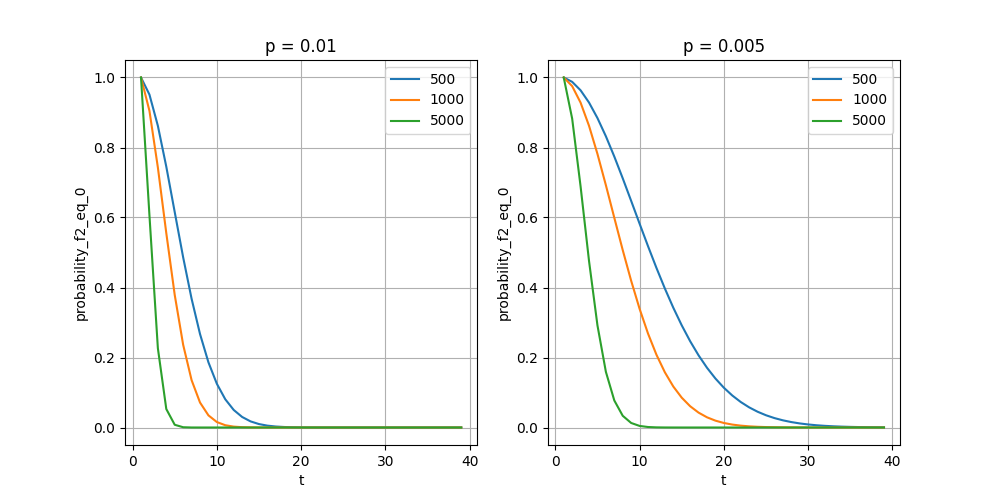
\includegraphics[width=\textwidth]{probability_f2_eq_0.png}
    % 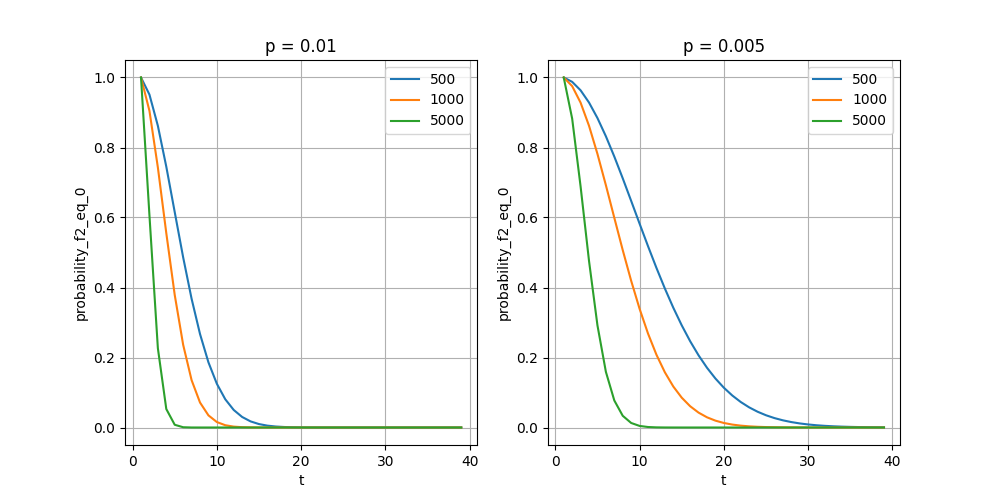
\includegraphics[\linewidth]{probability_f2_eq_0.png}
    \caption{Probability for $f_2 = 0$ over 40 times steps for different population sizes. Note that}
    \label{fig:probability_f2_eq_0_over_time}
\end{figure}

\begin{figure}[h]
    \centering
    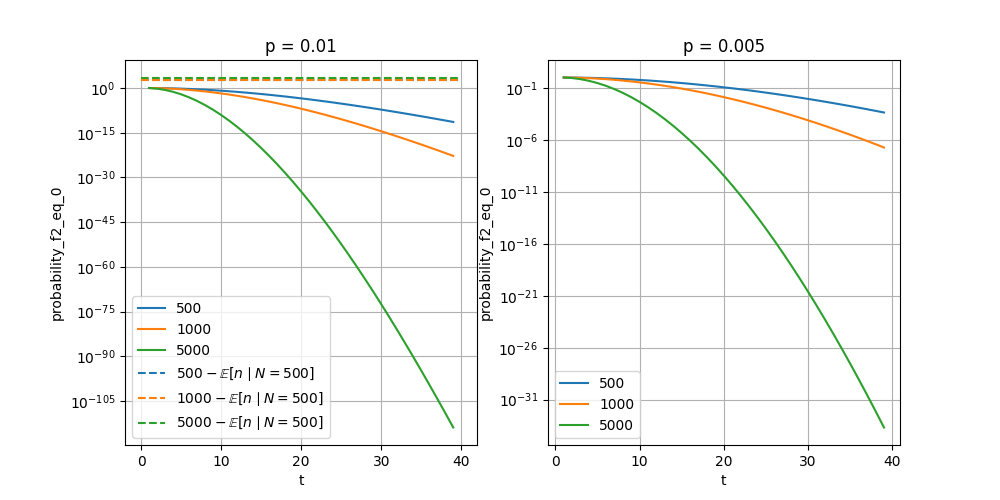
\includegraphics[width=\textwidth]{expectation_f0_f2_eq_0_rescaled.png}
    % 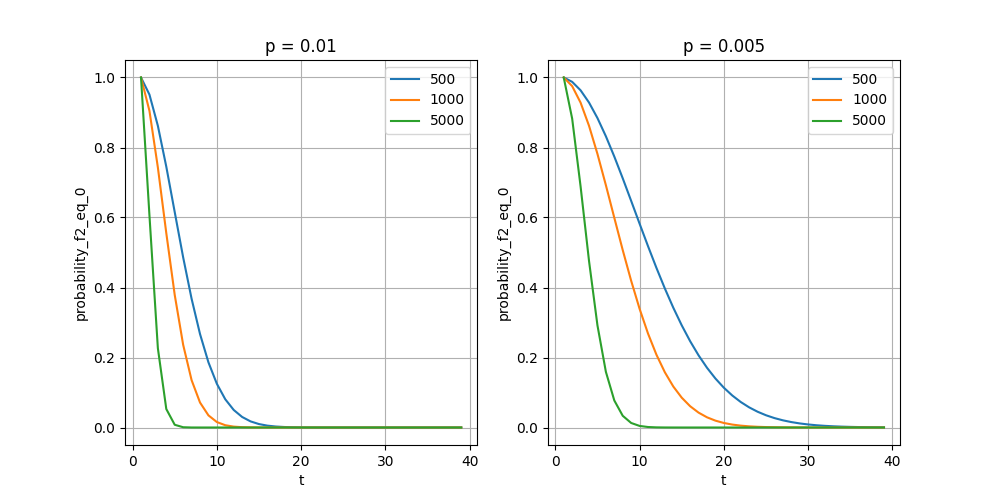
\includegraphics[\linewidth]{probability_f2_eq_0.png}
    \caption{The expected value for $\hat{f_0}$ conditioned on $f_2 = 0$ over 40 times steps for different population sizes. We multiply the expected value by the probability of $f_2 = 0$ at each time step.}
    \label{fig:expectation_f0_f2_eq_0_rescaled}
\end{figure}

\begin{figure}[h]
    \centering
    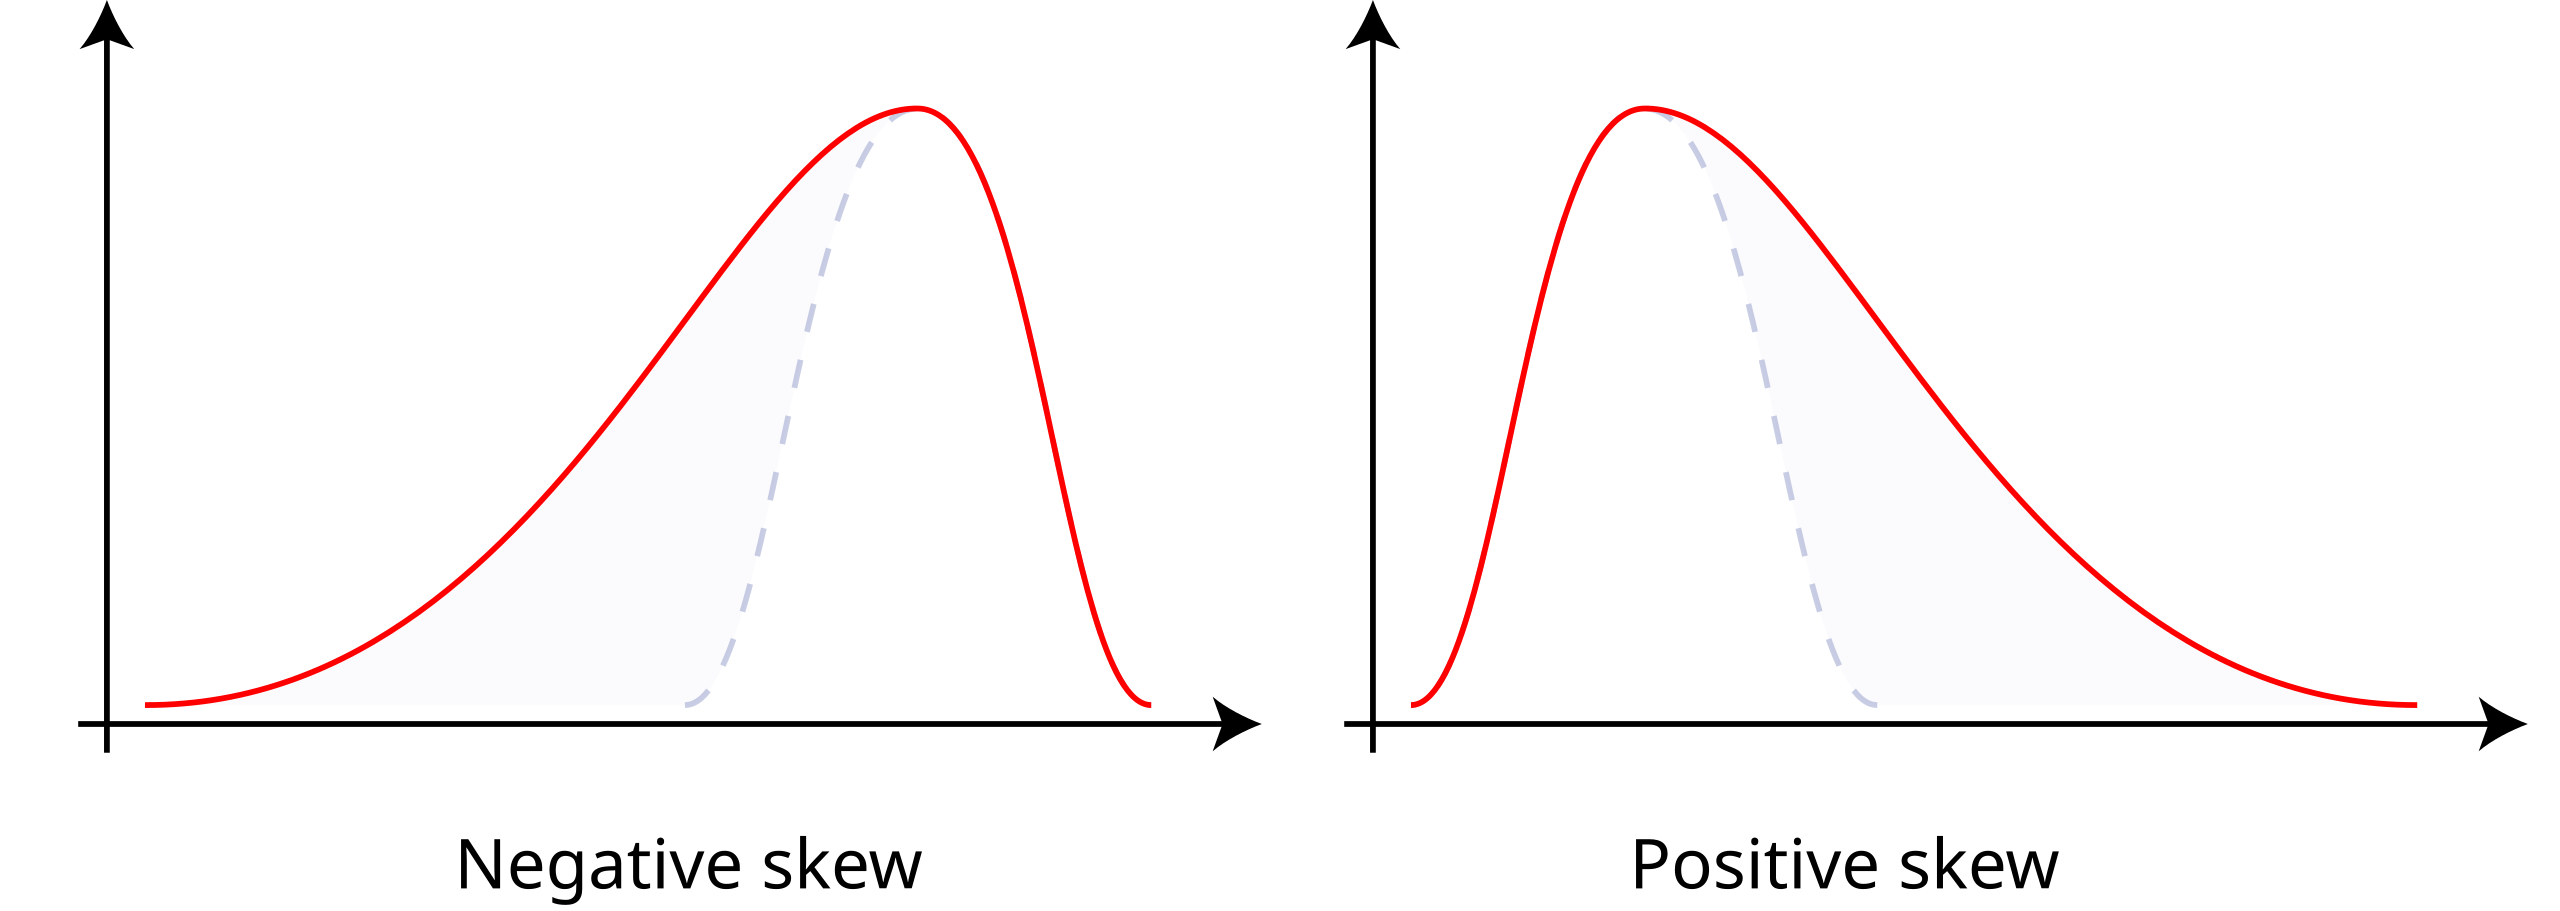
\includegraphics[width=\textwidth]{skewness.png}
    \caption{Interpretation of the skewness of a distribution.}
    \label{fig:interpretation_skewness}
\end{figure}

\pagebreak
\newpage
\subsection{Proof of the dependency of $f_1$ and $f_2$}
\label{sec:proof_dependency_f1_f2}

\begin{tcolorbox}[colframe=red!80!black, colback=red!10, boxrule=1pt, arc=4pt, left=6pt, right=6pt, top=4pt, bottom=4pt]
\textbf{Custom Note:} \\
The idea of this proof is to be credited to ChatGPT.

The current proof is just our own interpretation of the proof generated by ChatGPT, which we have deleted in the mean time.
\end{tcolorbox}

We can model the probability distribution of all $f_k$
jointly as a multinomial distribution.

In statistics, we can define two variables as independent if their covariance is zero.

From the multionomial distribution, we know that the covariance between $f_i$ and $f_j$ is given by 
\begin{equation*}
    \mathrm{Cov}(f_i, f_j) = -N p_i p_j\;.
\end{equation*}

Therefore, we have that 
\begin{align*}
    \mathrm{Cov}(f_1, f_2) &= -N p_1 p_2 \\
    &= -N \cdot \Pr(X_i = 1\mid T=t) \cdot \Pr(X_i = 2 \mid T=t) \\
    &= -N \cdot \mathrm{Binomial}(T, 1, p) \cdot \mathrm{Binomial}(T, 2, p)
\end{align*}
Naturally, we see that the Covariance is not zero, but slightly negative, and therefore the two variables are not independent.

For our four probability distributions, we have the following covariance values:
\begin{table}[h]
    \centering
    \begin{tabular}{c|c c c}
        \toprule
         & \multicolumn{3}{c}{$\mathrm{Cov}(f_1, f_2)$} \\
        \midrule
        $N$ & $500$ & $1000$ & $5000$ \\
        \midrule
        $p=0.01$  & $-7.20$   & $-14.39$  & $-71.95$ \\
        $p=0.005$ & $-1.33$   & $-2.65$   & $-13.26$ \\
        % \bottomrule
    \end{tabular}
    \caption{Covariance for $f_1$ and $f_2$ for $T=40$ and $N \in \{500, 1000, 5000\}$ for different values of $p$.}
    % \label{tab:covariance_f1_f2}
    % \label{tab:expected_value_f0_f2_eq_0}
\end{table}

From the multinomial distribution, we know that the variance of $f_i$ is given by
\begin{equation}
    V(f_i) = N p_i (1-p_i)\;. \label{eq:variance_f_i}
\end{equation}

Therefore, we can use Equation~\ref{eq:variance_f_i} to compute the correlation between $f_1$ and $f_2$ and report it in Table~\ref{tab:correlation_f1_f2}.
\begin{table}[h]
    \centering
    \begin{tabular}{c|c c c}
        \toprule
         & \multicolumn{3}{c}{$\mathrm{Corr}(f_1, f_2)$} \\
        \midrule
        $N$ & $500$ & $1000$ & $5000$ \\
        \midrule
        $p=0.01$  & $-0.1443$   & $-0.1443$  & $-0.1443$ \\
        $p=0.005$ & $-0.0568$   & $-0.0568$  & $-0.0568$ \\
        % \bottomrule
    \end{tabular}
    \caption{Covariance for $f_1$ and $f_2$ for $T=40$ and $N \in \{500, 1000, 5000\}$ for different values of $p$.}
    \label{tab:correlation_f1_f2}
    % \label{tab:expected_value_f0_f2_eq_0}
\end{table}

\qed

\section{Additional Plots and Tables}

\begin{figure}[H]
    \centering
    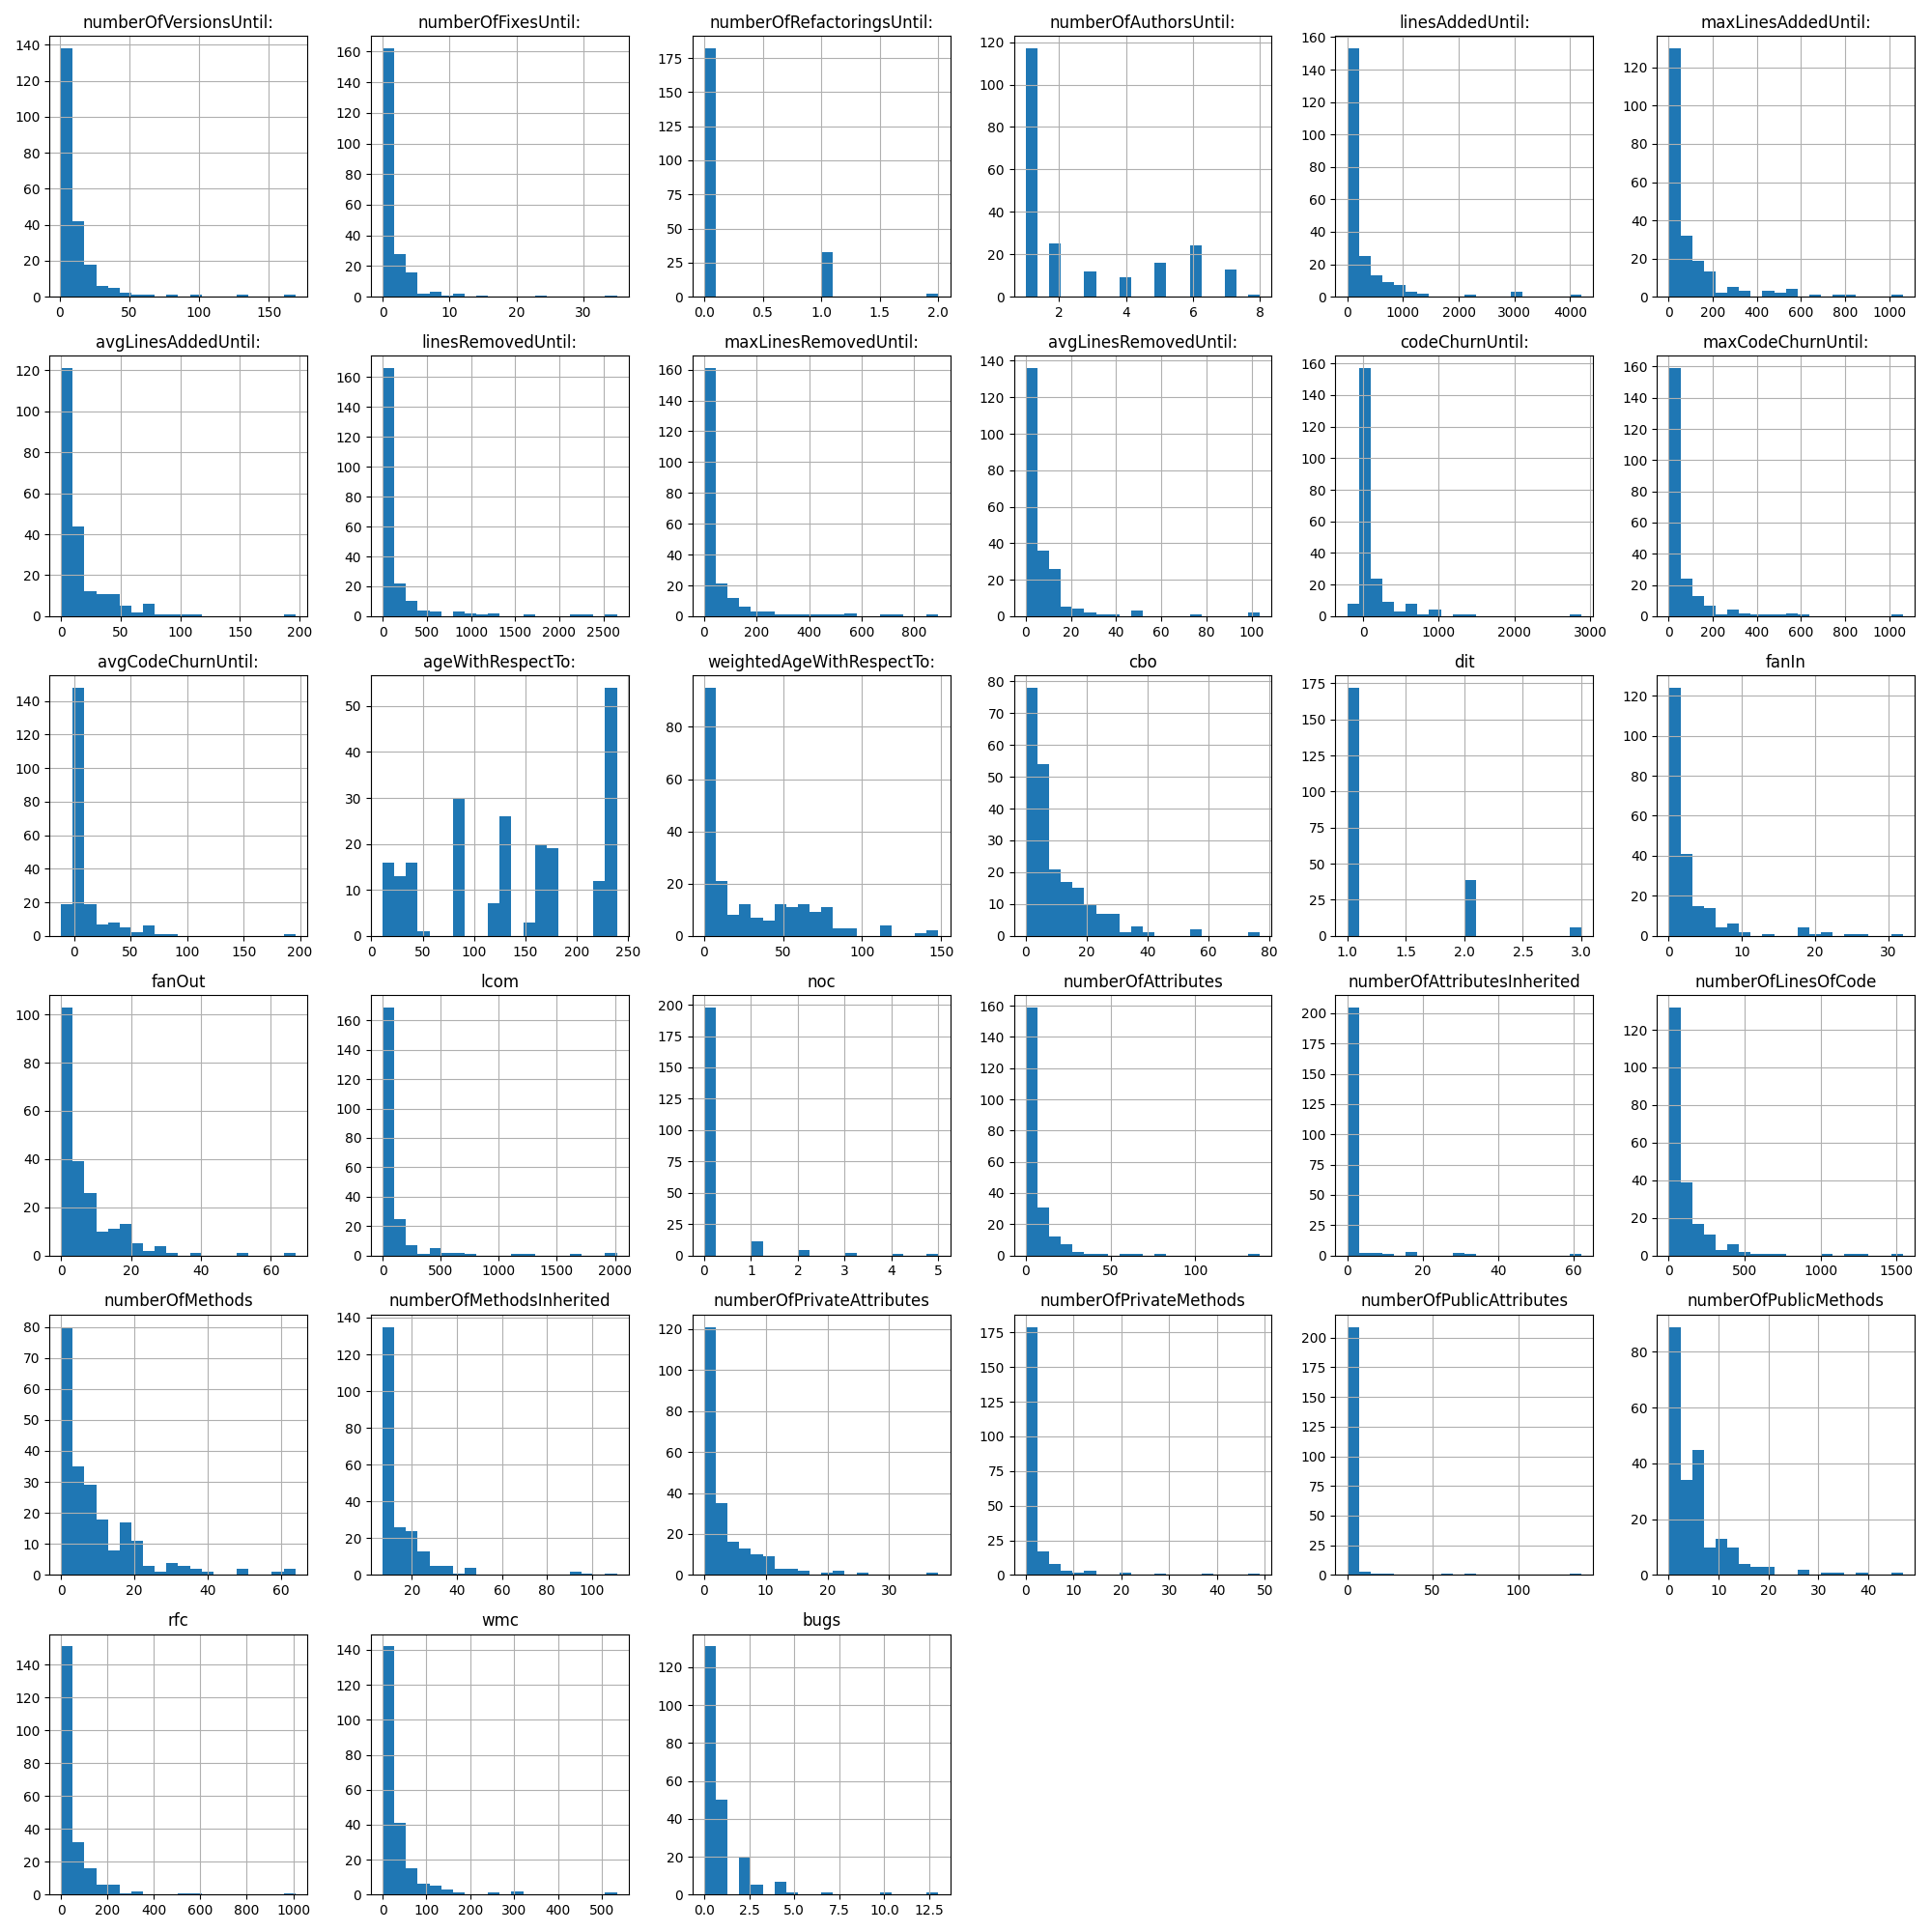
\includegraphics[width=\linewidth]{extra_plots/raw_feature_histograms.png}
    \caption{Histograms of the raw 32 features. No transformation has been applied.}
    \label{fig:feature_histogram_raw}
\end{figure}

\begin{figure}[t]
    \centering
    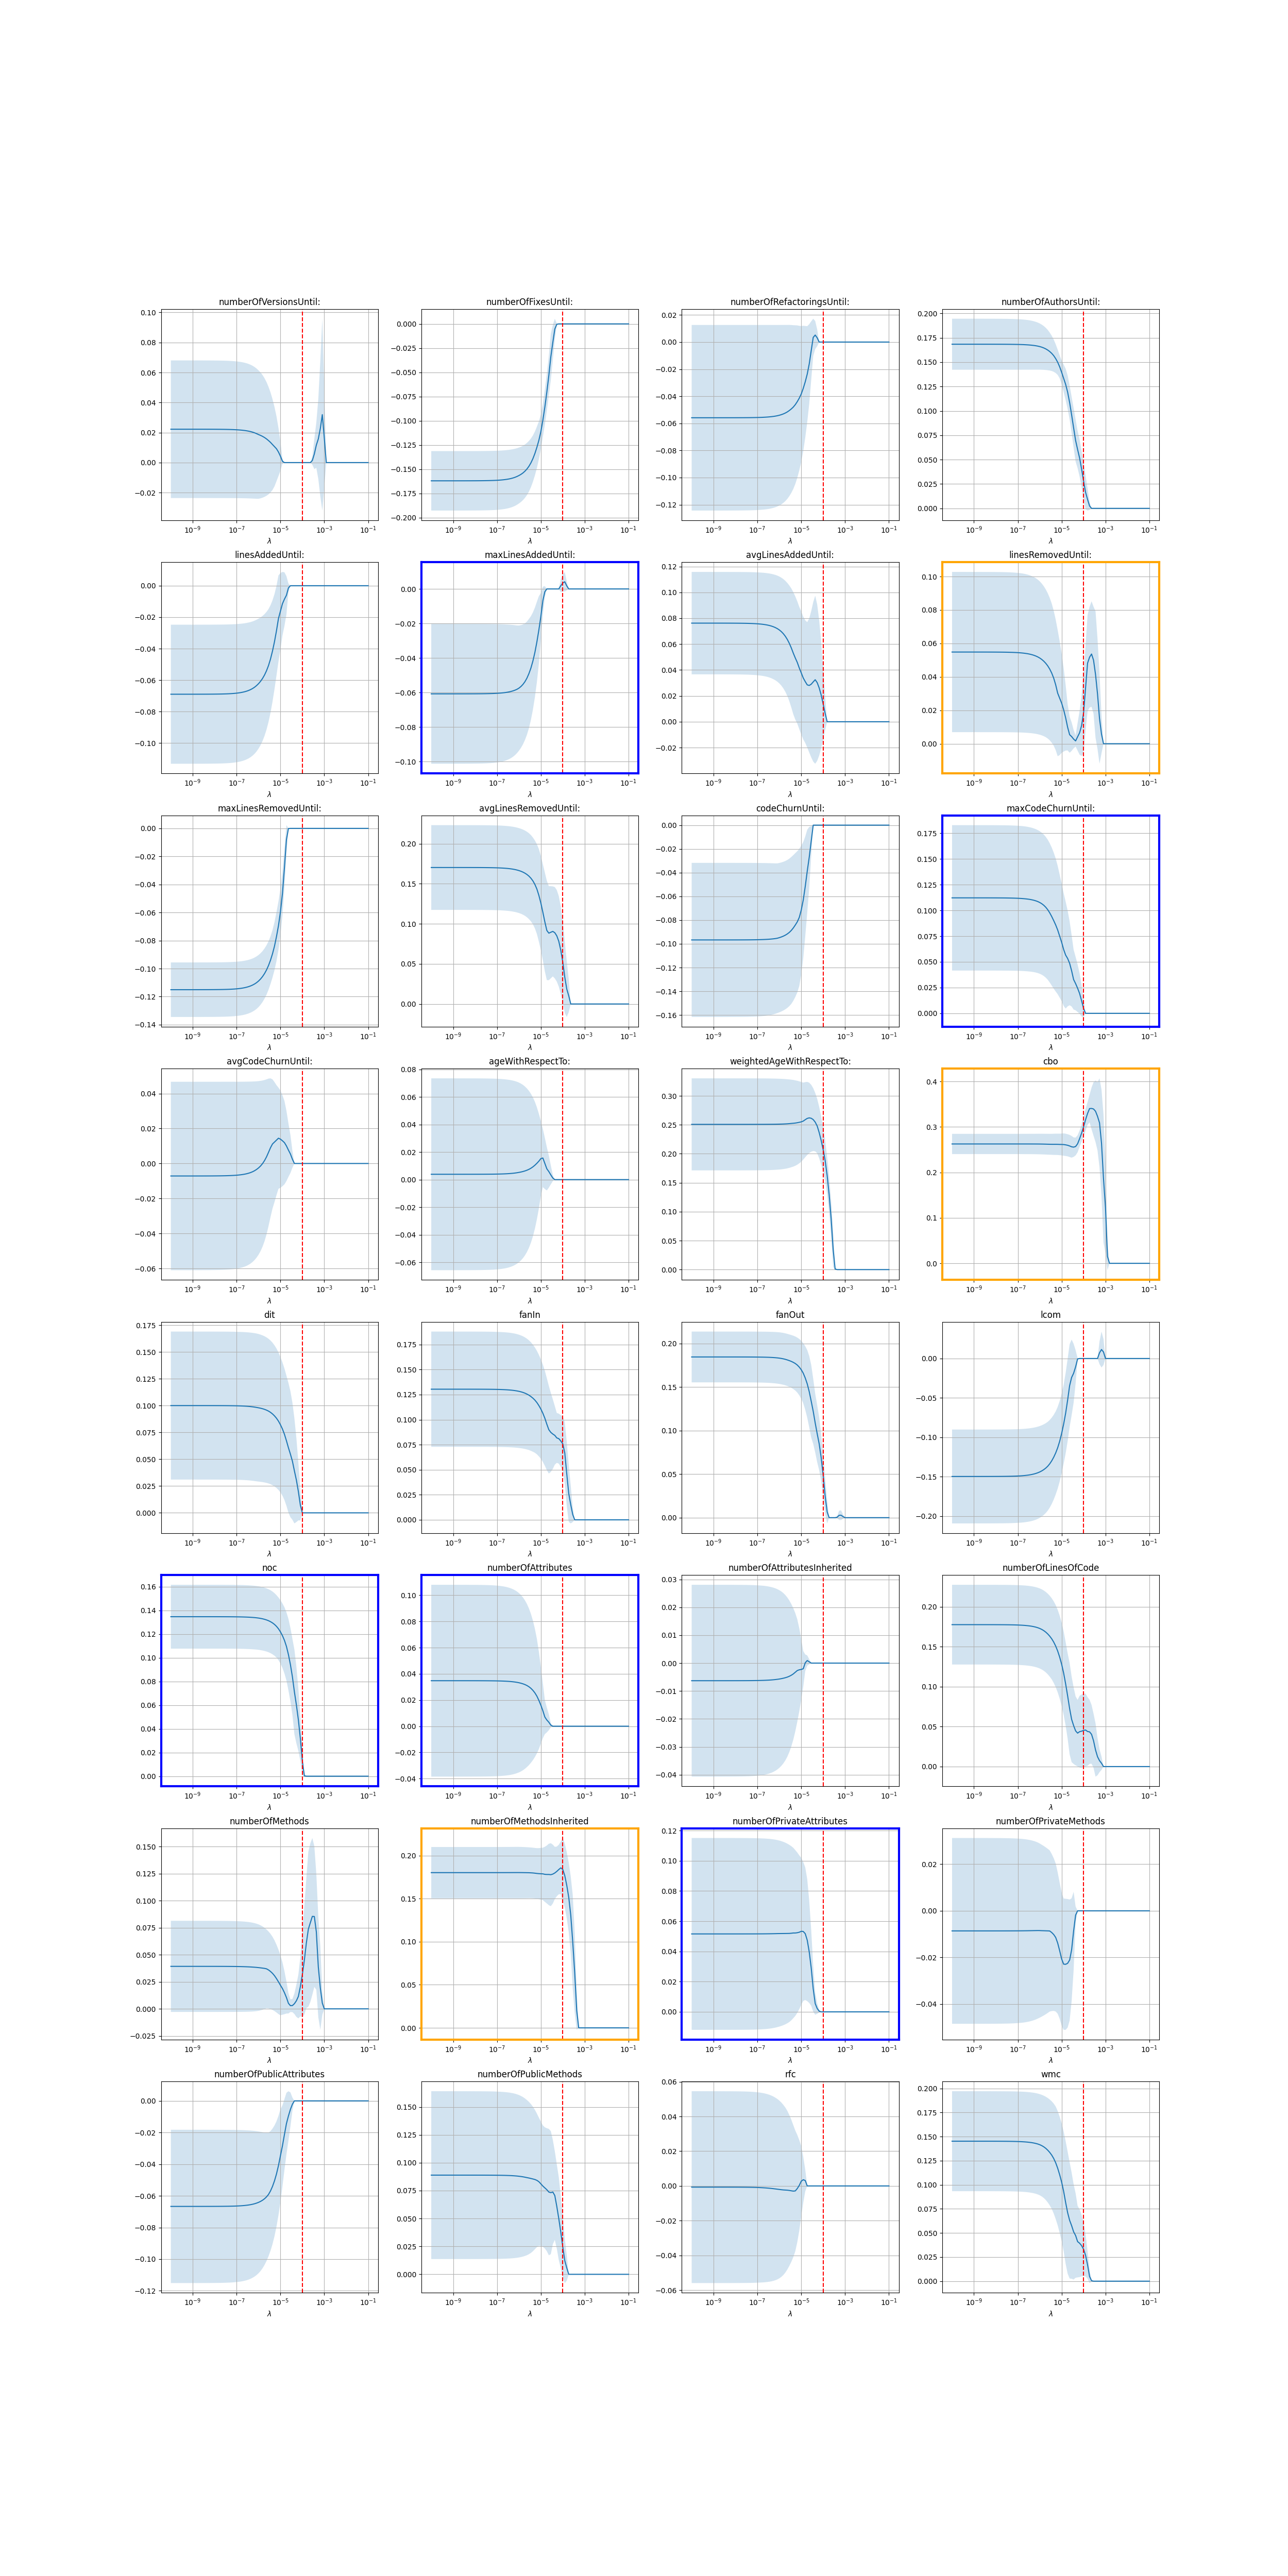
\includegraphics[width=0.5\linewidth]{extra_plots/poisson_regression_lasso_coefficients_no_log_transform.png}
    \caption{The coefficients of the \textbf{Poisson} regression model for all 32 features w.r.t. $\lambda$ when using the \textbf{normalized} data. The plots highlighted in \textbf{blue} are features found by the stepwise search model using AIC. We further highlighted in \textbf{orange} the features found by the stepwise search when using BIC. We advise the reader to view this report digitally to make the most of this plot.}
    \label{fig:coefficients_lambda_normalized}
\end{figure}

\begin{figure}[t]
    \centering
    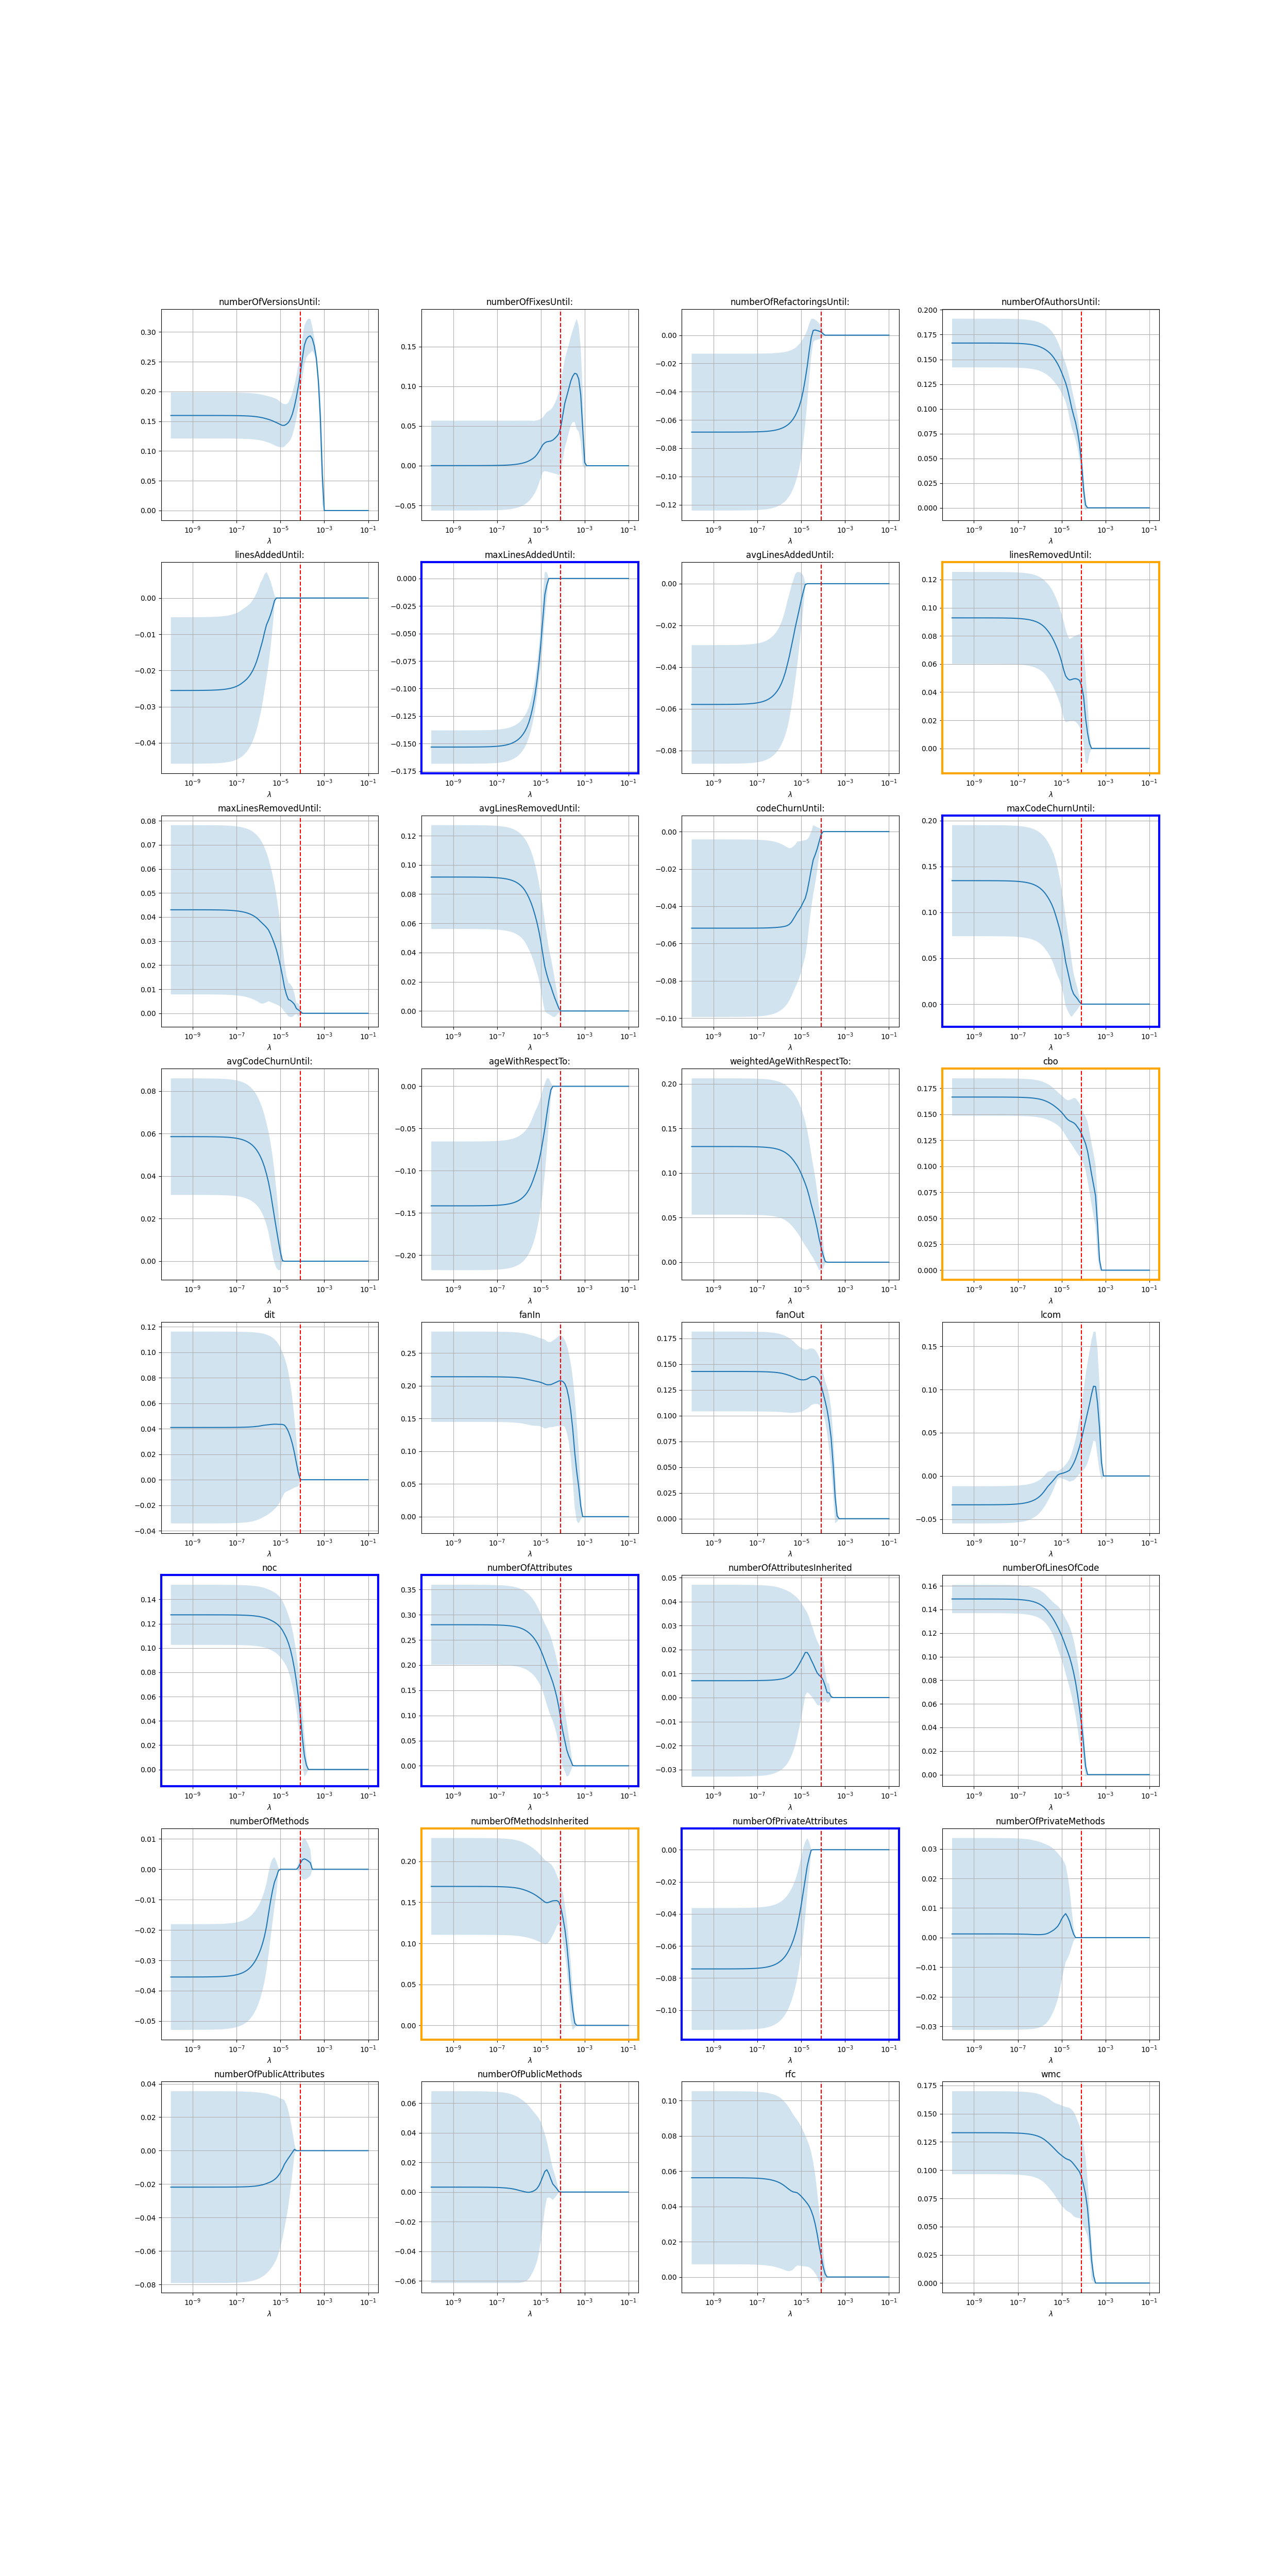
\includegraphics[width=0.5\linewidth]{extra_plots/poisson_regression_lasso_coefficients_log_transform.png}
    \caption{The coefficients of the \textbf{Poisson} regression model for all 32 features w.r.t. $\lambda$ when using the \textbf{log-transformed and normalized} data. The plots highlighted in \textbf{blue} are features found by the stepwise search model using AIC. We further highlighted in \textbf{orange} the features found by the stepwise search when using BIC. We advise the reader to view this report digitally to make the most of this plot.}
    \label{fig:coefficients_lambda_log_transformed_and_normalized}
\end{figure}

\begin{figure}[t]
    \centering
    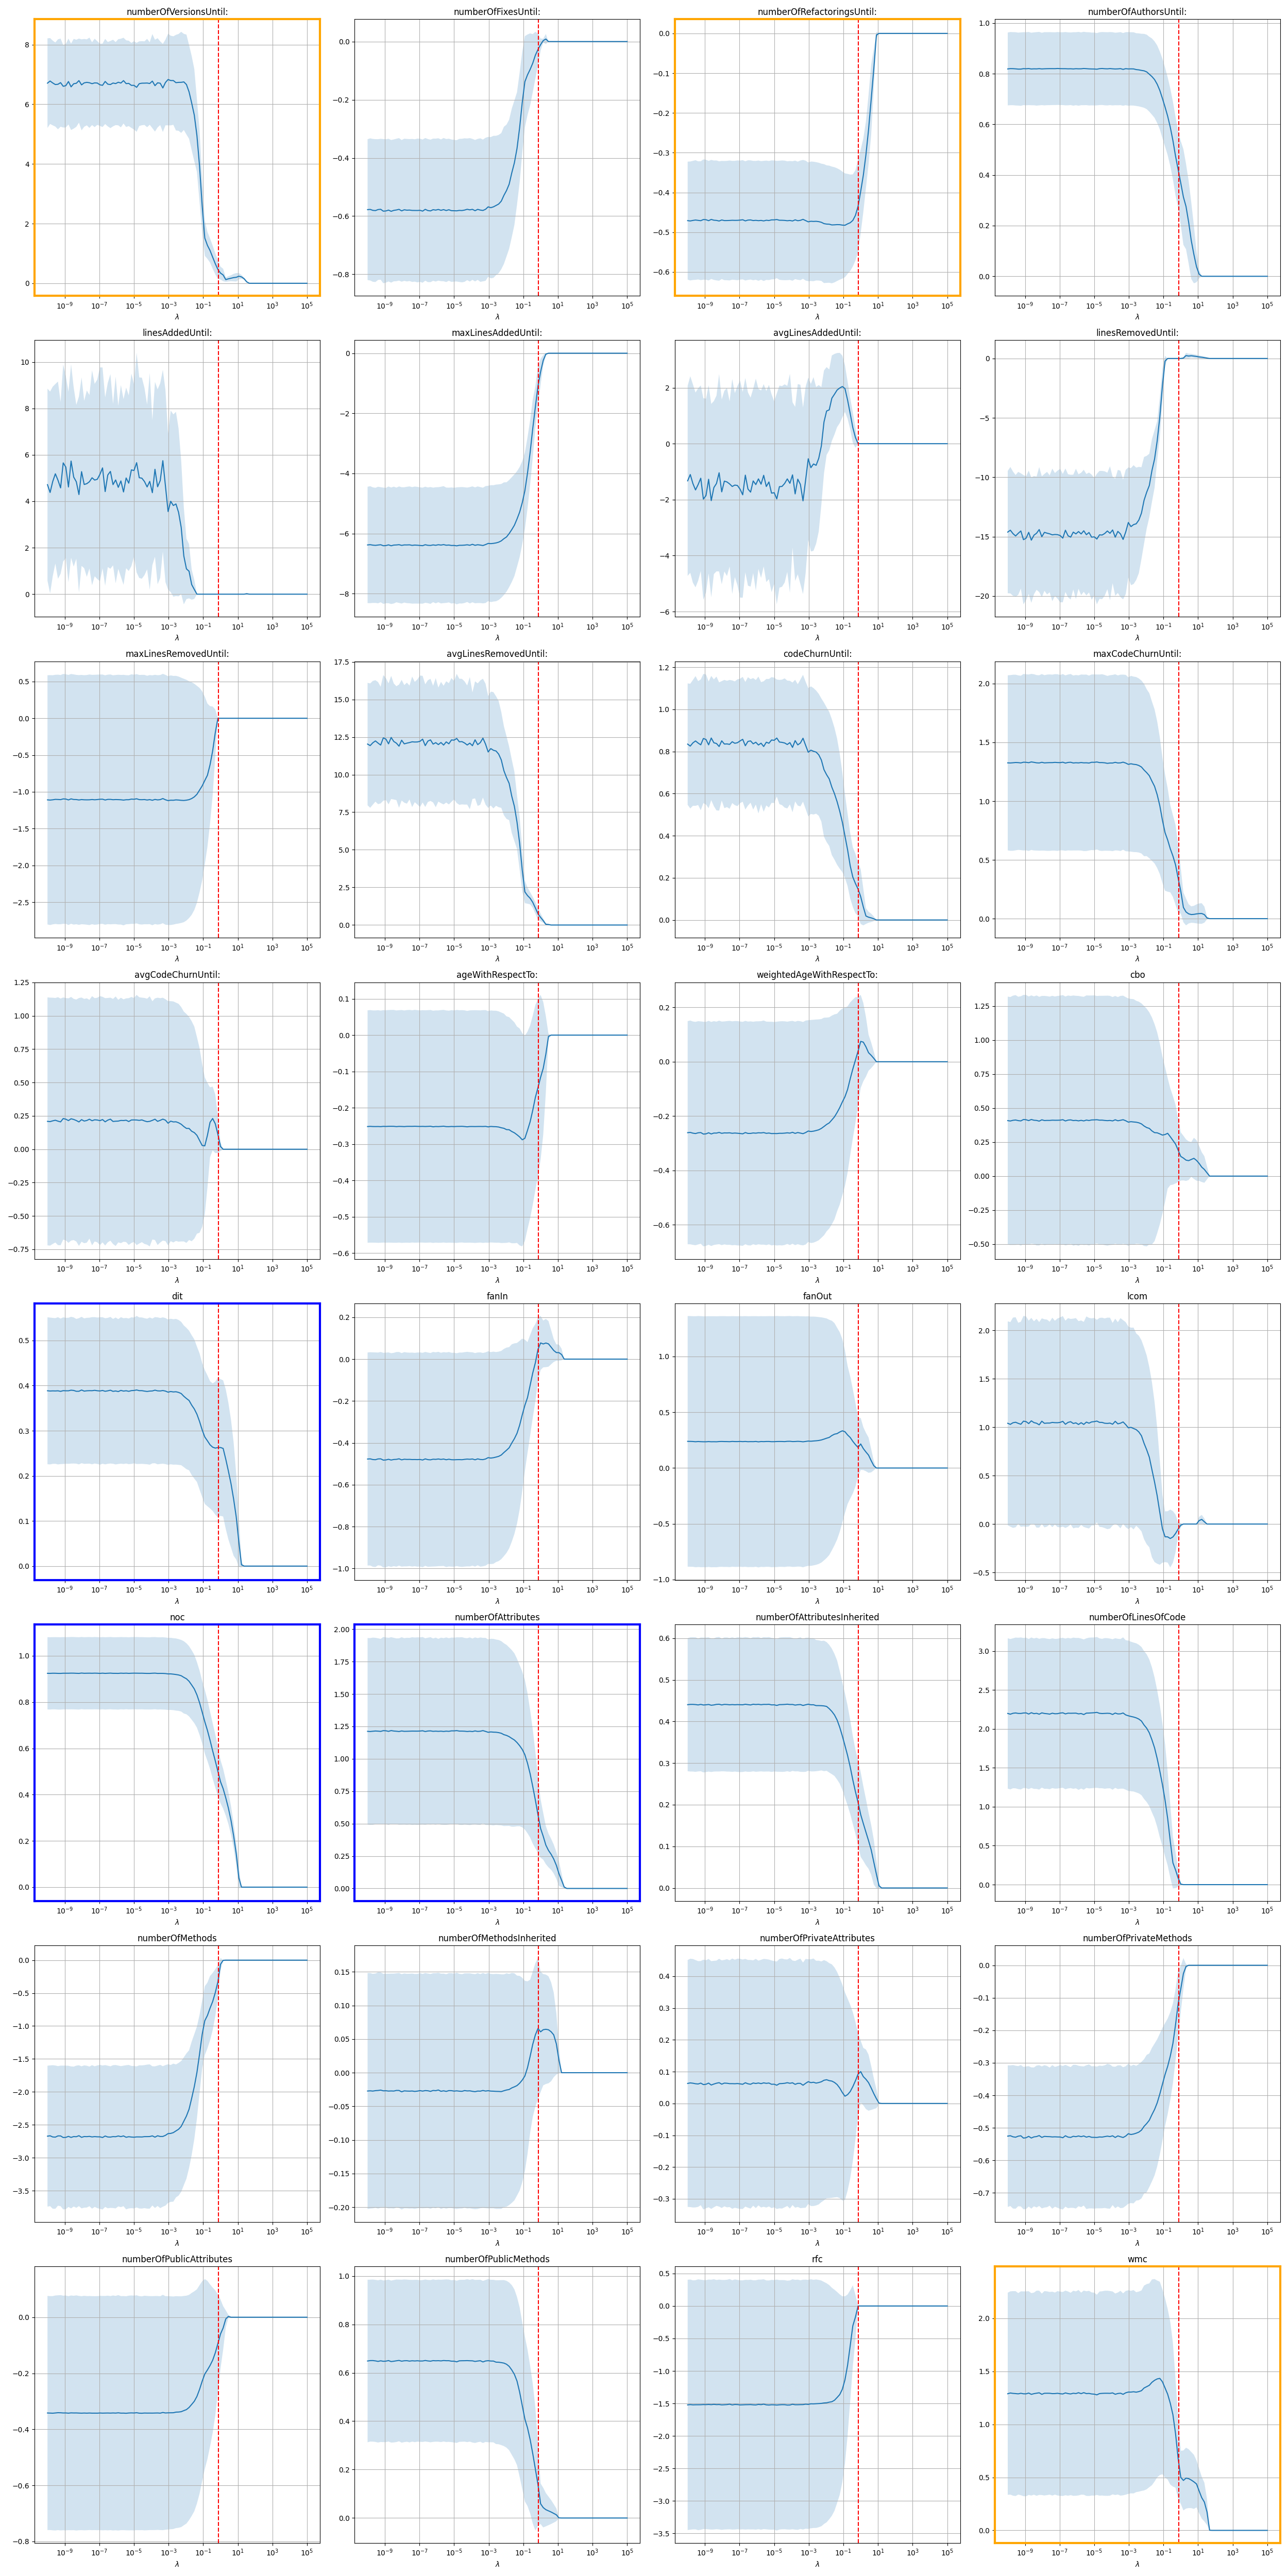
\includegraphics[width=0.5\linewidth]{extra_plots/logistic_regression_lasso_coefficients_log_transform.png}
    \caption{The coefficients of the \textbf{Logistic} regression model for all 32 features w.r.t. $\lambda$ when using the \textbf{log-transformed and normalized} data. The plots highlighted in \textbf{blue} are features found by the stepwise search model using AIC. We further highlighted in \textbf{orange} the features found by the stepwise search when using BIC. We advise the reader to view this report digitally to make the most of this plot.}
    \label{fig:logistic_regression_lasso_coefficients_log_transform}
\end{figure}

\begin{figure}[tp]
    \centering
    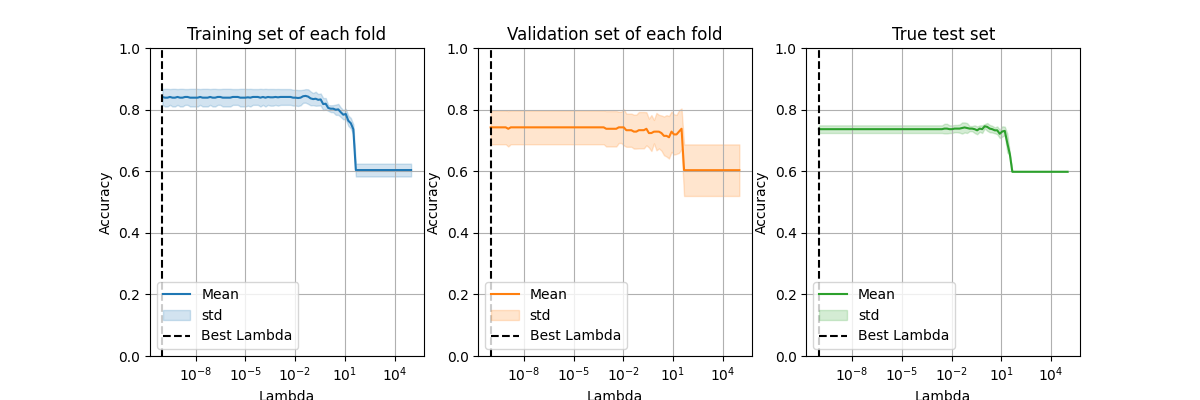
\includegraphics[width=\linewidth]{extra_plots/logistic_regression_lasso_deviance_vs_lambda_no_log_transform.png}
    \caption{Accuracy w.r.t. $\lambda$ for the $L_1$-lasso \textbf{logistic} regression for the just normalized data.}
    \label{fig:logistic_regression_lasso_deviance_vs_lambda_no_log_transform}
\end{figure}




\begin{table}[htbp]
    \centering
    \begin{tabular}{l c c}
        \toprule
        \textbf{Feature} & \textbf{Coefficient} & $\frac{\mathbb{E}[y\mid x+\delta_i]}{\mathbb{E}[y\mid x]}$ \\
        \midrule
        \texttt{noc} & $0.734$ & $3.335$ \\
        \texttt{dit} & $0.567$ & $3.219$ \\
        \texttt{cbo} & $3.020$ & $1.319$ \\
        \texttt{numberOfPublicMethods} & $1.631$ & $1.277$ \\
        \texttt{numberOfAuthorsUntil:} & $0.507$ & $1.269$ \\
        \texttt{numberOfPrivateMethods} & $0.654$ & $1.129$ \\
        \texttt{numberOfAttributes} & $0.932$ & $1.071$ \\
        \texttt{numberOfAttributesInherited} & $0.335$ & $1.059$ \\
        \texttt{wmc} & $2.731$ & $1.050$ \\
        \texttt{avgLinesRemovedUntil:} & $0.567$ & $1.044$ \\
        \texttt{numberOfPrivateAttributes} & $0.197$ & $1.039$ \\
        \texttt{numberOfMethodsInherited} & $0.333$ & $1.024$ \\
        \texttt{weightedAgeWithRespectTo:} & $0.384$ & $1.012$ \\
        \texttt{linesRemovedUntil:} & $3.676$ & $1.010$ \\
        \texttt{numberOfVersionsUntil:} & $0.175$ & $1.009$ \\
        \texttt{maxLinesAddedUntil:} & $1.290$ & $1.008$ \\
        \texttt{numberOfLinesOfCode} & $1.506$ & $1.007$ \\
        \texttt{lcom} & $0.988$ & $1.004$ \\
        \texttt{linesAddedUntil:} & $1.492$ & $1.003$ \\
        \texttt{maxCodeChurnUntil:} & $-0.261$ & $0.998$ \\
        \texttt{ageWithRespectTo:} & $-0.176$ & $0.998$ \\
        \texttt{codeChurnUntil:} & $-0.819$ & $0.997$ \\
        \texttt{avgLinesAddedUntil:} & $-0.197$ & $0.992$ \\
        \texttt{avgCodeChurnUntil:} & $-0.252$ & $0.988$ \\
        \texttt{maxLinesRemovedUntil:} & $-2.965$ & $0.977$ \\
        \texttt{rfc} & $-3.512$ & $0.966$ \\
        \texttt{numberOfPublicAttributes} & $-1.004$ & $0.916$ \\
        \texttt{fanOut} & $-1.009$ & $0.894$ \\
        \texttt{fanIn} & $-1.324$ & $0.763$ \\
        \texttt{numberOfMethods} & $-3.550$ & $0.727$ \\
        \texttt{numberOfFixesUntil:} & $-1.390$ & $0.670$ \\
        \texttt{numberOfRefactoringsUntil:} & $-0.542$ & $0.258$ \\
        \bottomrule
    \end{tabular}
    \caption{Coefficients of the best \textbf{Logistic} regression model found with \textbf{$L_1$-regularization} for the \textbf{just normalized} dataset.}
    \label{tab:features_coeff_logistic_normalized}
\end{table}



% I used ChatGPT to help find literature on the properties of integration, differentiation.

% Furthermore, when researching for denoising algorithms, I used ChatGPT to get a general overview of the available general denoising algorithms. After finding the Bayesian denoising algorithm, I used Claude 4.5 Sonnet to write the code for the Bayesian denoising algorithm (based on existing code for Bayesian denoising implemented for 2D images). As the exact algorithm is not at the core of the assignment or the course, and that the results of both denoising methods are very similar, I believe that this usage is acceptable.

\end{document}
